\documentclass{article}

\usepackage[utf8]{inputenc}

\usepackage{amsmath, bm}
\usepackage{graphicx}
\usepackage{amssymb}
\usepackage{float}
\usepackage{caption}
\usepackage{subcaption}
\usepackage{hyperref}
\usepackage{tikz}
\usepackage{layout}
\usepackage{booktabs}

\usepackage[margin=1in]{geometry}
\usepackage{listings}
\usepackage{xcolor}
\usepackage{color, colortbl}
\usepackage{textgreek}
\usepackage{mathrsfs}
\usepackage{savetrees}[moderate]
\usepackage{dirtree}
\usepackage{adjustbox}


\usetikzlibrary{calc}
\usetikzlibrary{angles,quotes} % for pic
\usetikzlibrary{patterns,snakes}
\usetikzlibrary{arrows}
\tikzset{>=latex} % for LaTeX arrow head

\setlength{\parskip}{\baselineskip}%
\setlength{\parindent}{0pt}%
\linespread{0.9}


\definecolor{codegreen}{rgb}{0,0.6,0}
\definecolor{codegray}{rgb}{0.5,0.5,0.5}
\definecolor{codepurple}{rgb}{0.58,0,0.82}
\definecolor{backcolour}{rgb}{0.95,0.95,0.92}

\lstdefinestyle{mystyle}{
    backgroundcolor=\color{backcolour},   
    commentstyle=\color{codegreen},
    keywordstyle=\color{magenta},
    numberstyle=\tiny\color{codegray},
    stringstyle=\color{codepurple},
    basicstyle=\ttfamily\footnotesize,
    breakatwhitespace=false,         
    breaklines=true,                 
    captionpos=b,                    
    keepspaces=true,                 
    numbers=left,                    
    numbersep=5pt,                  
    showspaces=false,                
    showstringspaces=false,
    showtabs=false,                  
    tabsize=2
}

\lstset{style=mystyle}



\begin{document}

\title{Computational Fluid Dynamics \\
    \large Final Report}
\author{lwp26}
\date{December 2024}
\maketitle 

\section{Introduction}

% make better
Computational Fluid Dynamics (CFD) is a powerful tool for solving fluid flow problems.
This can be done much faster and at lower cost than experimental methods.
This makes it a valuable tool to be used alongside experimental validation.


\section{Objective}

%To write a program to solve the Euler equations for two-dimensional flows using a finite volume time
%marching method. Completing this work will give you practical expertise in pre-processing and post-
%processing the simulations as well as understanding the methods of solution. The knowledge gained
%is core to all CFD methods and transferrable to all other research and commercial CFD packages

\begin{itemize}
    \item Write a program to solve the Euler equations for two-dimensional flows using a finite volume time marching method.
    \item Pre-process and post-process the simulations.
    \item Understand the methods of solution.
    \item Gain practical expertise in CFD methods.
\end{itemize}

\section{Software}
% monumental amount of work required here
\subsection{Modifications}
% interpolate
% write_settings python

Some corrections were made to the code supplied by the course.
The first correction was to the \texttt{interpolate} fortran function to fix an issue which only presented when compiling without debug symbols which made it difficult to identify.
It was found that in some cases this function was returning unset memory values at the last point of the array. This is believed to be due to more relaxed precision in \texttt{si} which left it outside the normalised range of \texttt{si\_a}.
The fix was to add a check to see if \texttt{si} is outside the input range, and if so return the boundary value.
Another correction in the python function \texttt{write\_settings} was also made where the gas constants were being written in the incorrect order.

The general program \texttt{stopit} file was removed and replaced with the boolean \texttt{av\%crashed} which is set to \texttt{True} if \texttt{NaN} is detected, or if the user interrupts the program.
Not only is this more efficient, but also now allows cases to be run in parallel; writing only to case specific files, and not a shared program file that causes write violations.
This was imporant to accelerate the testing and a custom python thread pool manager was written for this purpose.
A worker creates the directory structure for the case, runs the solver, and then writes the key results to a shared file.
The worker directory and run function are shown in the appendix \ref{fig:worker_dir}.
The number of threads in the threadpool was set to 8, less than the number of cores on the machine to prevent incorrect time measurements due to windows thread scheduling.

The GUI was improved with more inputs and improved visualisation animations.
The zoom and pan no longer resets on each frame update and is consistent between tabs.

\subsection{Convergence definition}

The same convergence criteria described in the Interim report \cite{interim} was implemented to stop the solver when the last 100 calculated \texttt{d\_avg} were all within a factor of \texttt{d\_var} of their mean.
This was done to prevent the solver from reaching max iterations when the solution had already converged, making it possible to more accurately measure the runtime.
Large values of \texttt{d\_var}, can cause the solver to stop prematurely if the convergence was slow, and similarly small values
can cause the solver to run for longer than necessary.
Additionally the requirement of 100 points of \texttt{d\_avg}, which is calculated every 50 iterations means that the minimum number of iterations for convergence to be detected is 5000.
With the improvements made convergence was, for some cases, observed to occur before this limit, highlighting a problem with the convergence criteria.

The original check if the final residual error is within the bounds specified in the inputs is nested within this check.
This means the solver subroutine will terminate with 4 possible outcomes:
\begin{itemize}
    \item Converged within boundary specified
    \item Converged outside boundary specified
    \item Diverged
    \item Maximum iterations reached
\end{itemize}

\subsection{Figure of merit definition}
In order to identify the best parameters, its useful to define a figure of merit (FM) to compare the performance of the code.
In our case we want the most accuracy in the least amount of time and so the FM is defined as
\begin{equation}
    \text{FM} = \log_{10} \left( \frac{1}{\texttt{d\_avg} \times T} \right)
\end{equation}

\subsection{Improvements}
% runge kutta
% deferred correction
% residual averaging
% spatially varying timestep
\subsubsection{Runge-Kutta}

The Runge-Kutta methods are a family of implicit and explicit iterative methods used to solve ordinary differential equations.
This involves computing gradients at a number of intermediate timesteps to improve accuracy of each timestep.
The method implemented here is informal in that the gradients are between the starting timestep property and previous intermediate timestep property.
Another difference to typical RK4 is that the intermediate timesteps linearly increase to total timestep size in a method similar to 3/8-rule.
This method, also proposed by Kutta, has advantages compared to typical RK4 in that most error coefficients are smaller however, the method is more computationally expensive \cite{solve_ODE_nonstiff}.


\subsubsection{Deferred Correction}

The amount of smoothing required for stability decreases as the solution converges to steady state.
This means over many iterations we can start to reduce the amount of artifical viscosity added to the solution.
This can be done by defining another flow correction variable, \texttt{corr}, that slowly approaches a final correction factor
\begin{equation}
    \texttt{corr\_total} = \texttt{fcorr} \times (\texttt{prop} - \texttt{prop\_average}).
\end{equation}
Then \texttt{corr} is updated by
\begin{equation}
    \texttt{corr} = (1 - \texttt{corr\_rate}) \times \texttt{corr} + \texttt{corr\_rate} \times \texttt{corr\_total}
\end{equation}
Each iteration the solution then is smoothed towards \texttt{prop\_average} + \texttt{corr}.

The amount of artifical viscosity cancelled out is set by \texttt{fcorr} and the rate of correction is set by \texttt{corr\_rate}.
However, \texttt{corr\_rate} was fixed within the solver to 0.01.

\subsubsection{Residual Averaging}

At the onset of instability the adjacent grid points have high and low respective values that causes the solution to oscillate on alternating timesteps.
If the timestep is too large the amplitude of these oscillations can grow and cause the solution to diverge.
Its possible to smooth the changes in primary flow variables to improve stability.
This is done by
\begin{equation}
    \texttt{dcell} = (1 - \texttt{sfac\_res}) \times \texttt{dcell} + \texttt{sfac\_res} \times \texttt{dcell\_avg}
\end{equation}
This should allow for larger \texttt{cfl} numbers and so converge faster. 

\subsubsection{Spatially Varying Timestep}

Steady state is reached when the change in variables between cells converges to the residual value.
This condition can occur at each cell for different timesteps.
The current global timestep is calculated from the global minimum cell size and so is significantly smaller than the maximum stable local timestep for many cells.
If a steady state solution is all that is required then convergence can be accelerated by using the local timestep for each cell.
This would be calculated below
\begin{equation}
    \Delta t = \frac{l_{min}}{a + v}
\end{equation}
Where $l_{min}$ is the minimum between the cell length and height, $a$ is the local speed of sound, and $v$ is the local velocity of the fluid.
The local timesteps are then updated every 10 iterations.
While this marginally increases the time per iteration, it reduces the number of iterations required to converge.


\subsection{Extension}
% multigrid
% talk a bit about external flows
% comparison to boundary element methods e.g. SA1 spoilers its much less useful
% important cases evaluation turbinne_c represent same geometry with different
% mesh shapes make a large impact on the compuational effort accuracy curve.
% identify and make some recommonendations on mesh geometry


\subsection{Additional Case}
% airfoil case comparison with SA1 or xfoil
% experiment with airfoils
The generate naca case function was modified to input the 4 digit naca airfoil code to generate various airfoil geometries.
A simpler symmetric airfoil case, NACA0012 was tested to compare with the provided NACA2412 case.

% compare turbine theory with turbo course

\section{Results}

Unless otherwise specified the following default parameters are used for the cases:
% big table

\begin{table}[H]
    \begin{adjustbox}{tabular=l|rrrrrrrrrrrr,center}
        \texttt{casename} & \texttt{cfl} & \texttt{sfac} & \texttt{sfac\_res} & \texttt{fcorr} & \texttt{nsteps} & \texttt{ni} & \texttt{nj} & \texttt{pstag} & \texttt{tstag} & \texttt{alpha} & \texttt{rfin} & \texttt{p} \\
        \hline
        bend & 0.20 & 0.80 & 0.50 & 0.90 & 1e+05 & 53 & 37 & 1.00e+05 & 300.00 & 0.0 & 0.25 & 8.50e+04 \\
        bump & 0.80 & 0.80 & 0.50 & 0.90 & 1e+05 & 53 & 37 & 1.00e+05 & 300.00 & 0.0 & 0.25 & 8.50e+04 \\
        naca0012 & 0.20 & 0.60 & 0.50 & 0.60 & 1e+05 & - & - & 1.00e+05 & 300.00 & 0.0 & 0.25 & 9.00e+04 \\
        naca2412 & 0.05 & 0.60 & 0.50 & 0.60 & 1e+05 & - & - & 1.00e+05 & 300.00 & 0.0 & 0.25 & 9.00e+04 \\
        turbine\_c & 0.10 & 0.60 & 0.50 & 0.80 & 1e+05 & - & - & 1.05e+05 & 300.00 & 0.0 & 0.25 & 1.03e+05 \\
        turbine\_h & 0.10 & 0.80 & 0.00 & 0.90 & 1e+05 & - & - & 1.05e+05 & 300.00 & 0.0 & 0.10 & 1.03e+05 \\
    \end{adjustbox}
    \caption{Default parameters for cases. \texttt{d\_max} = 1e-4 and \texttt{d\_var} = 1e-2 for all cases.}   
    \label{tab:default_params}
\end{table}

\subsection{Comparison of Improvements}

\begin{figure}[H]
    \centering
    \begin{subfigure}{0.49\textwidth}
        \centering
        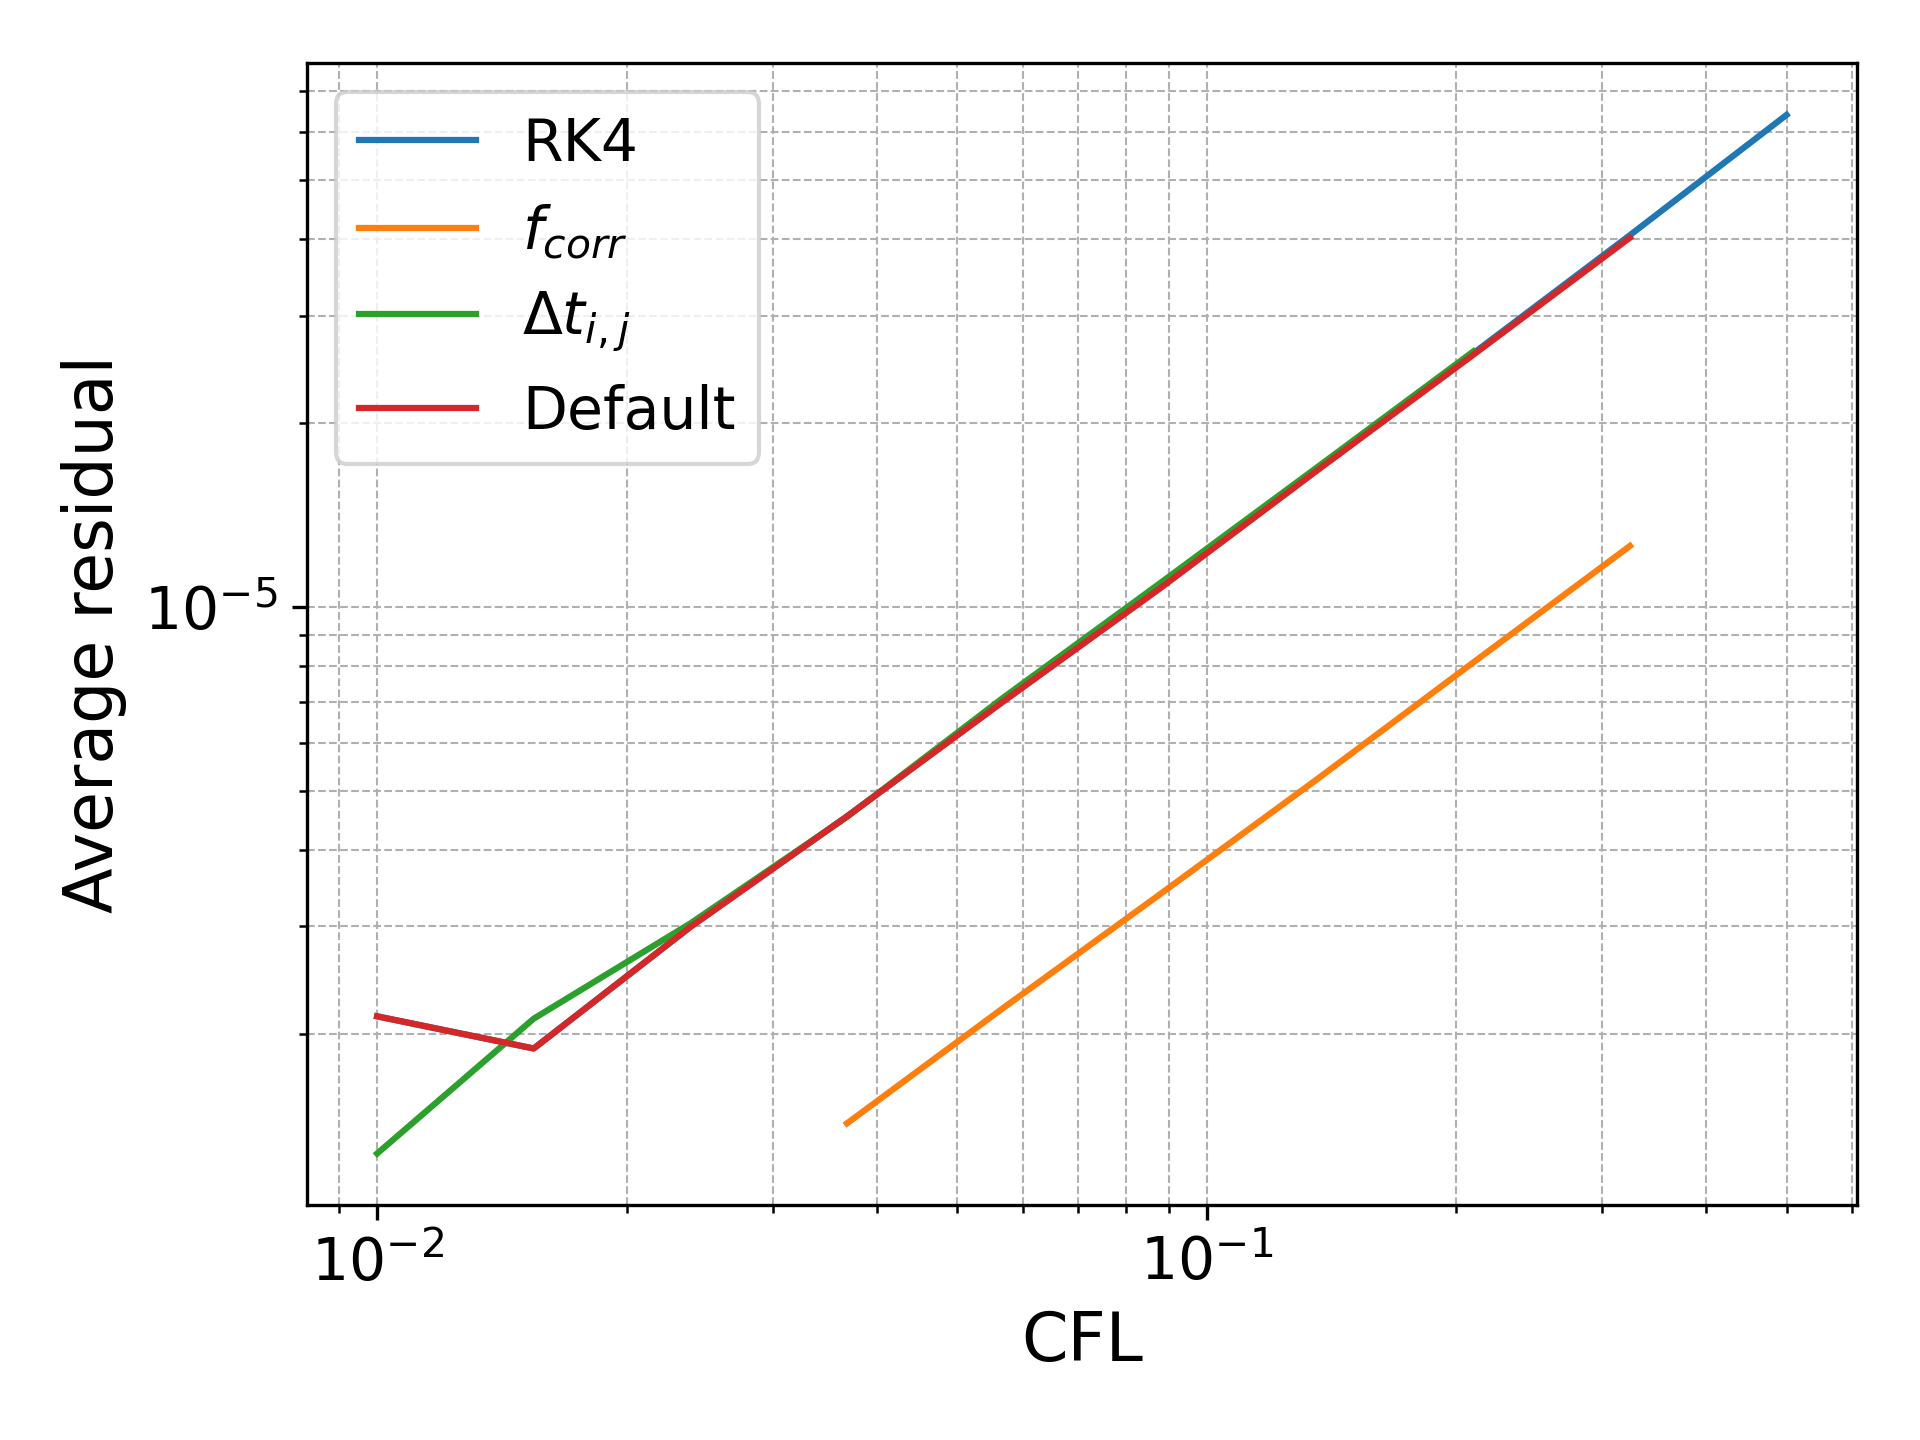
\includegraphics[width=0.99\textwidth]{figures/improvements_cfl_residual.png}
        \caption{Varying \texttt{cfl} with \texttt{ni} = 53}
        \label{fig:improvements_cfl_residual}
    \end{subfigure}
    \begin{subfigure}{0.49\textwidth}
        \centering
        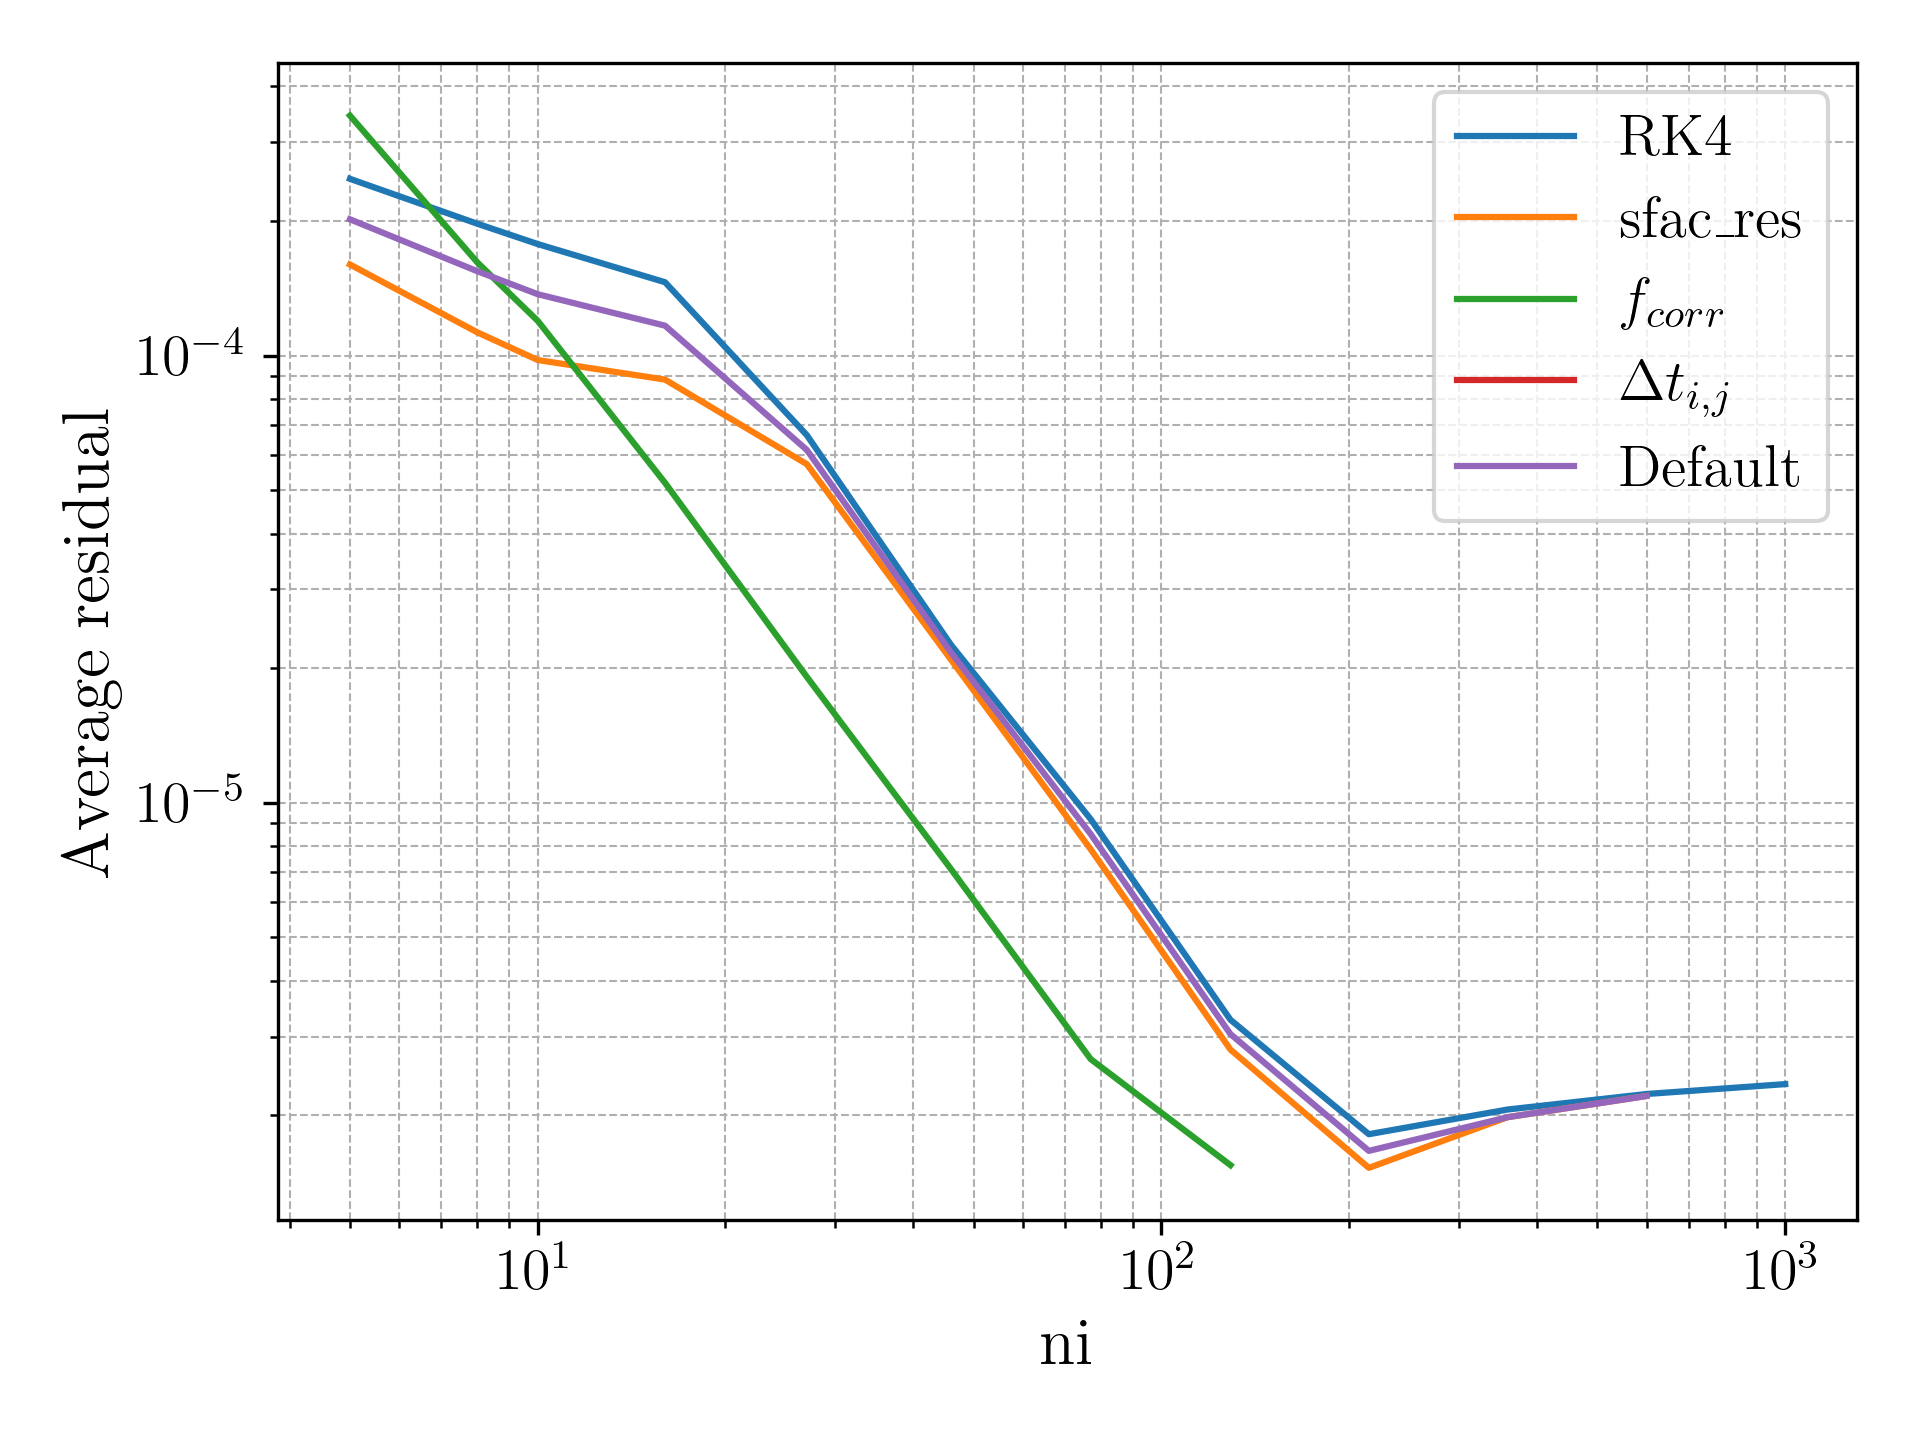
\includegraphics[width=0.99\textwidth]{figures/improvements_ni_residual.png}
        \caption{Varying \texttt{ni} with \texttt{cfl} = 0.2}
        \label{fig:improvements_ni_residual}
    \end{subfigure}
    \caption{Spatial and temporal accuracy of improvements}
\end{figure}

\begin{figure}[H]
    \centering
    \begin{subfigure}{0.49\textwidth}
        \centering
        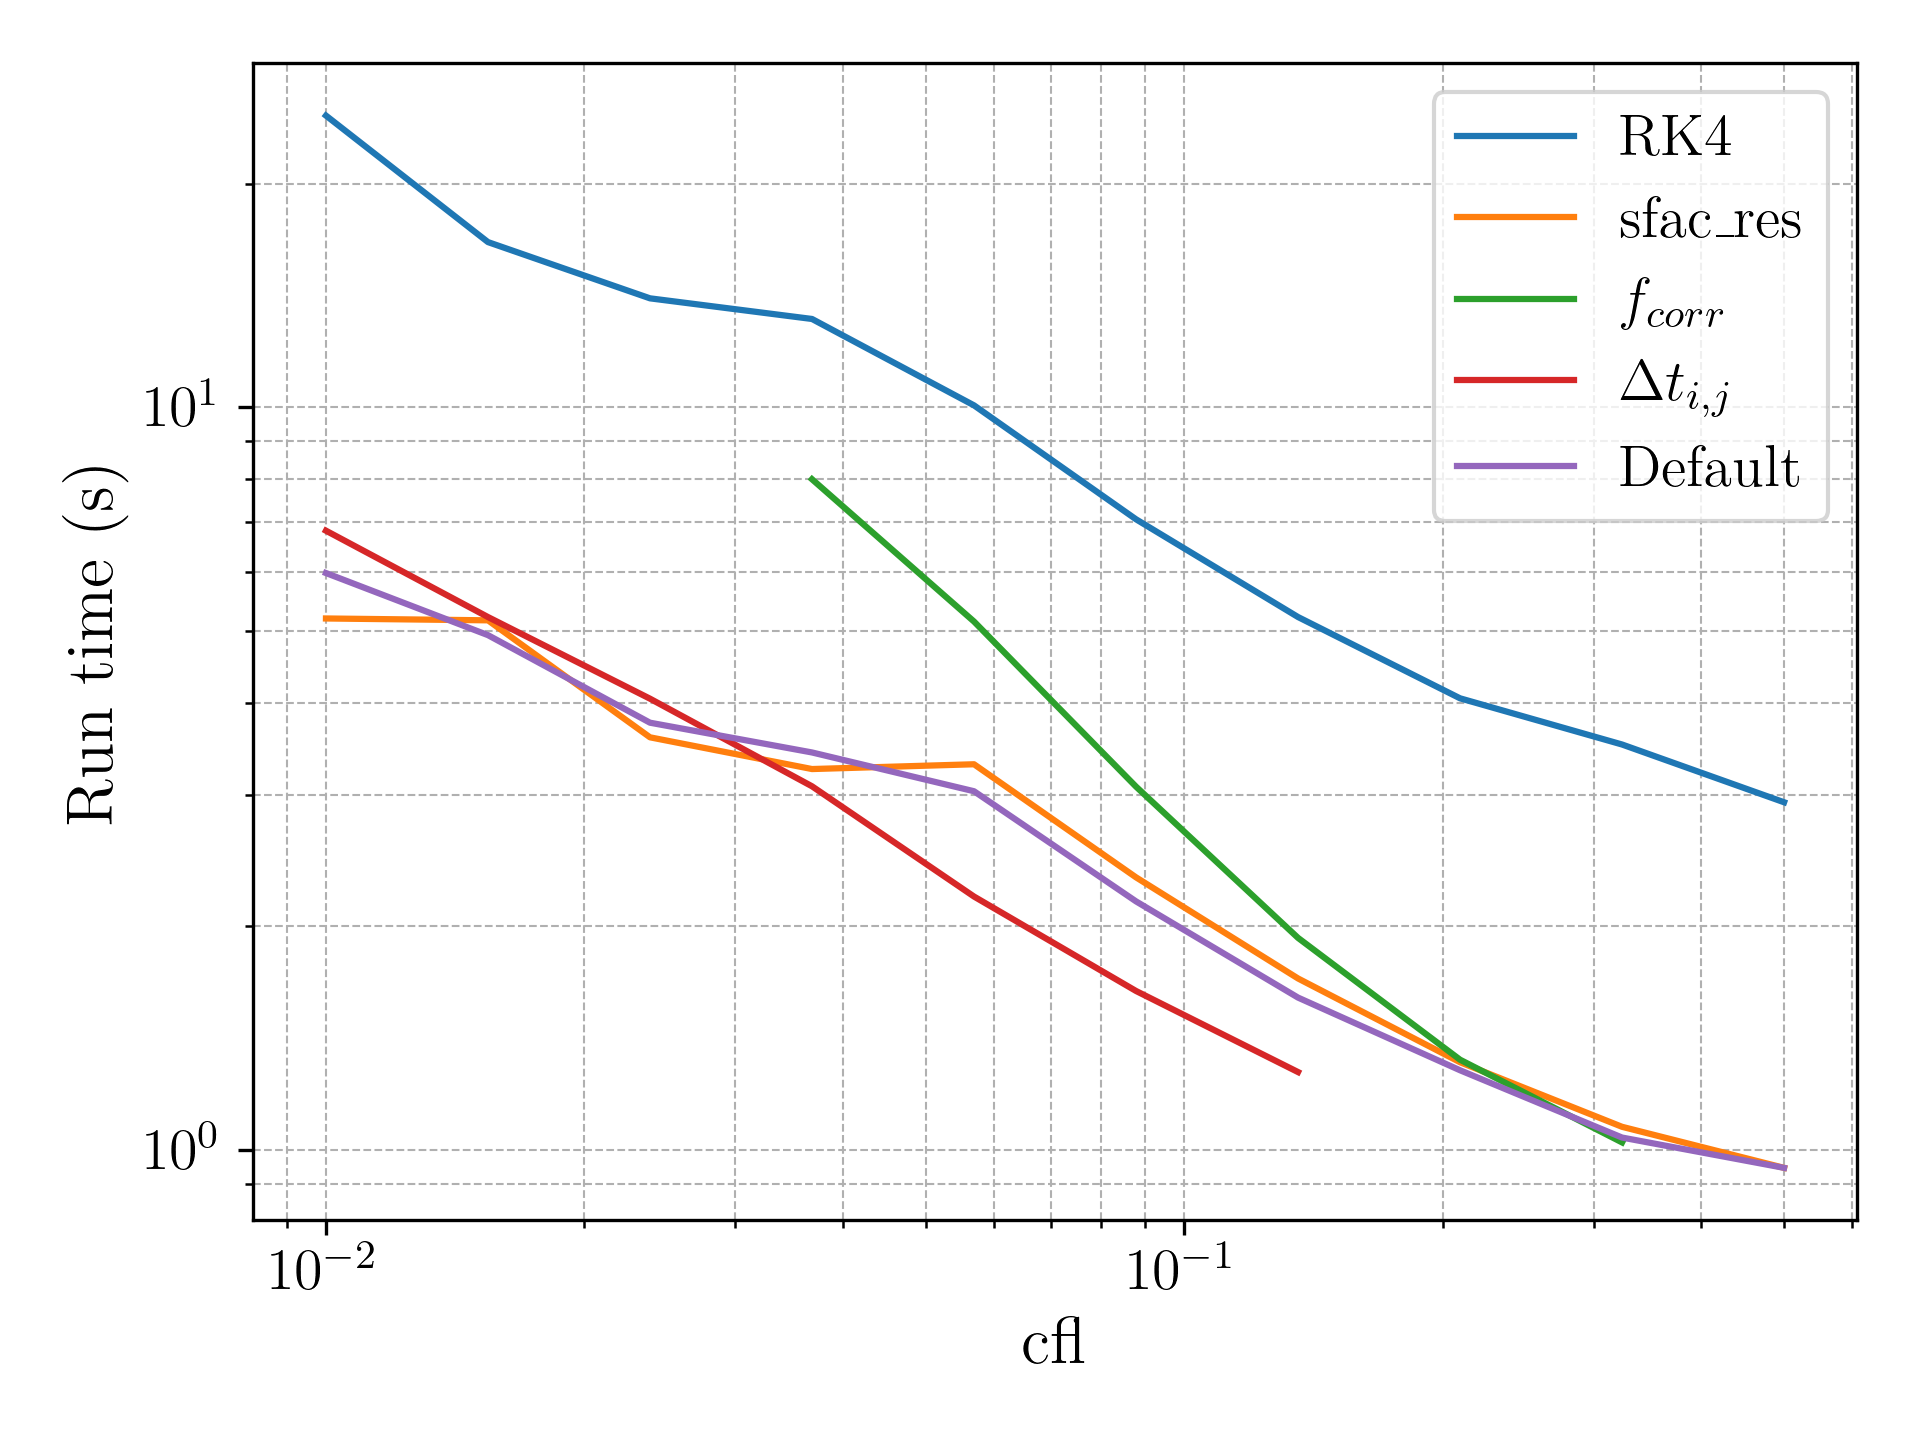
\includegraphics[width=0.99\textwidth]{figures/improvements_cfl_time.png}
        \caption{Varying CFL number}
        \label{fig:improvements_cfl_time}
    \end{subfigure}
    \begin{subfigure}{0.49\textwidth}
        \centering
        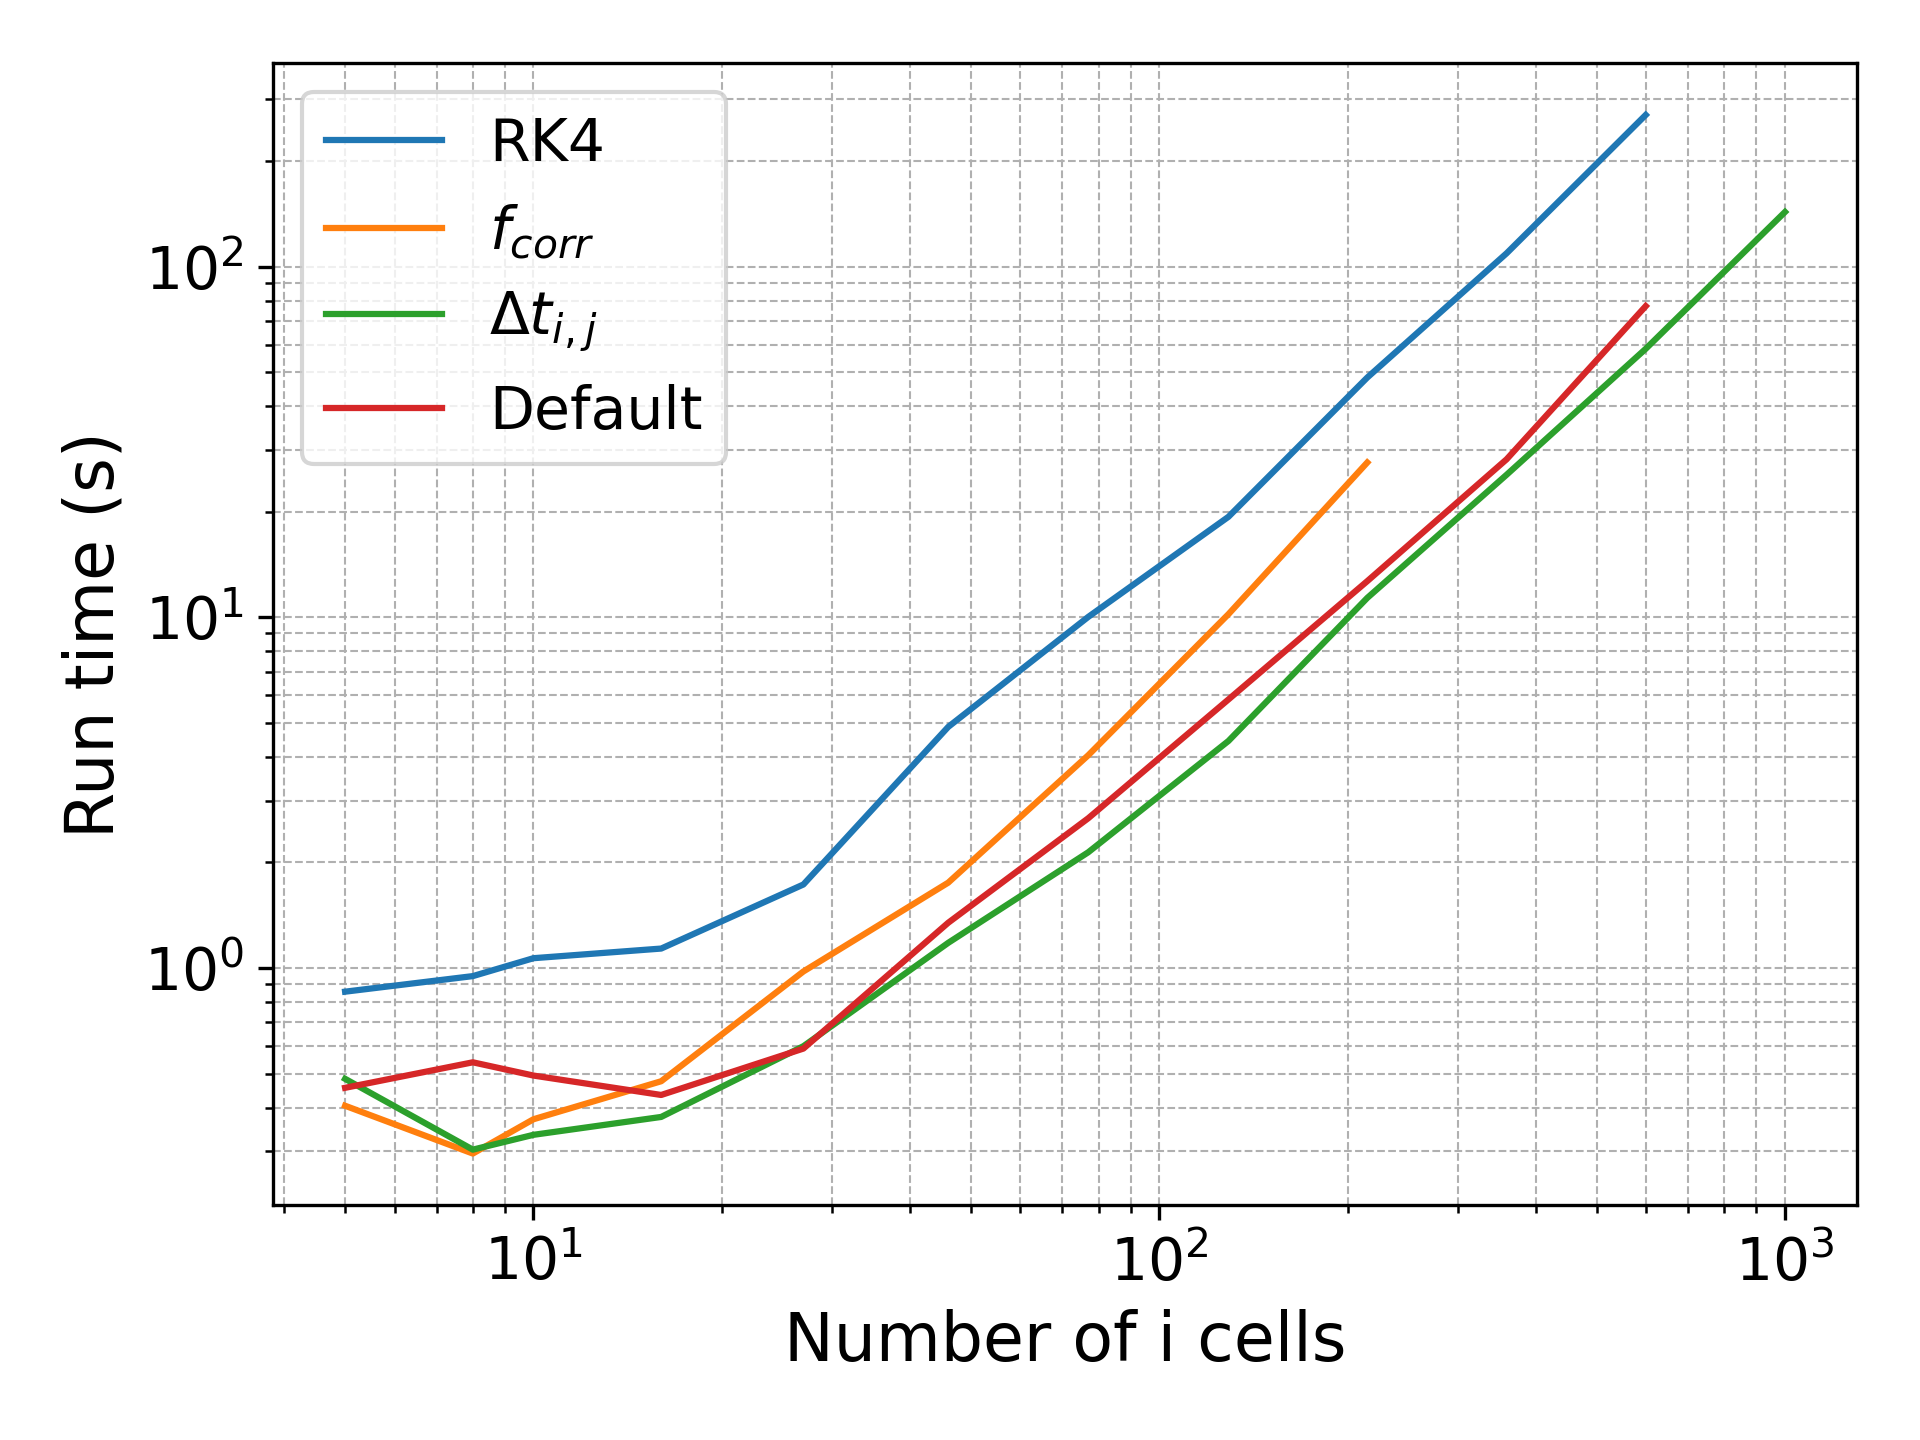
\includegraphics[width=0.99\textwidth]{figures/improvements_ni_time.png}
        \caption{Varying number of cells in \texttt{i} direction}
        \label{fig:improvements_ni_time}
    \end{subfigure}
    \caption{Spatial and temporal impact on runtime}
\end{figure}

\begin{figure}[H]
    \centering
    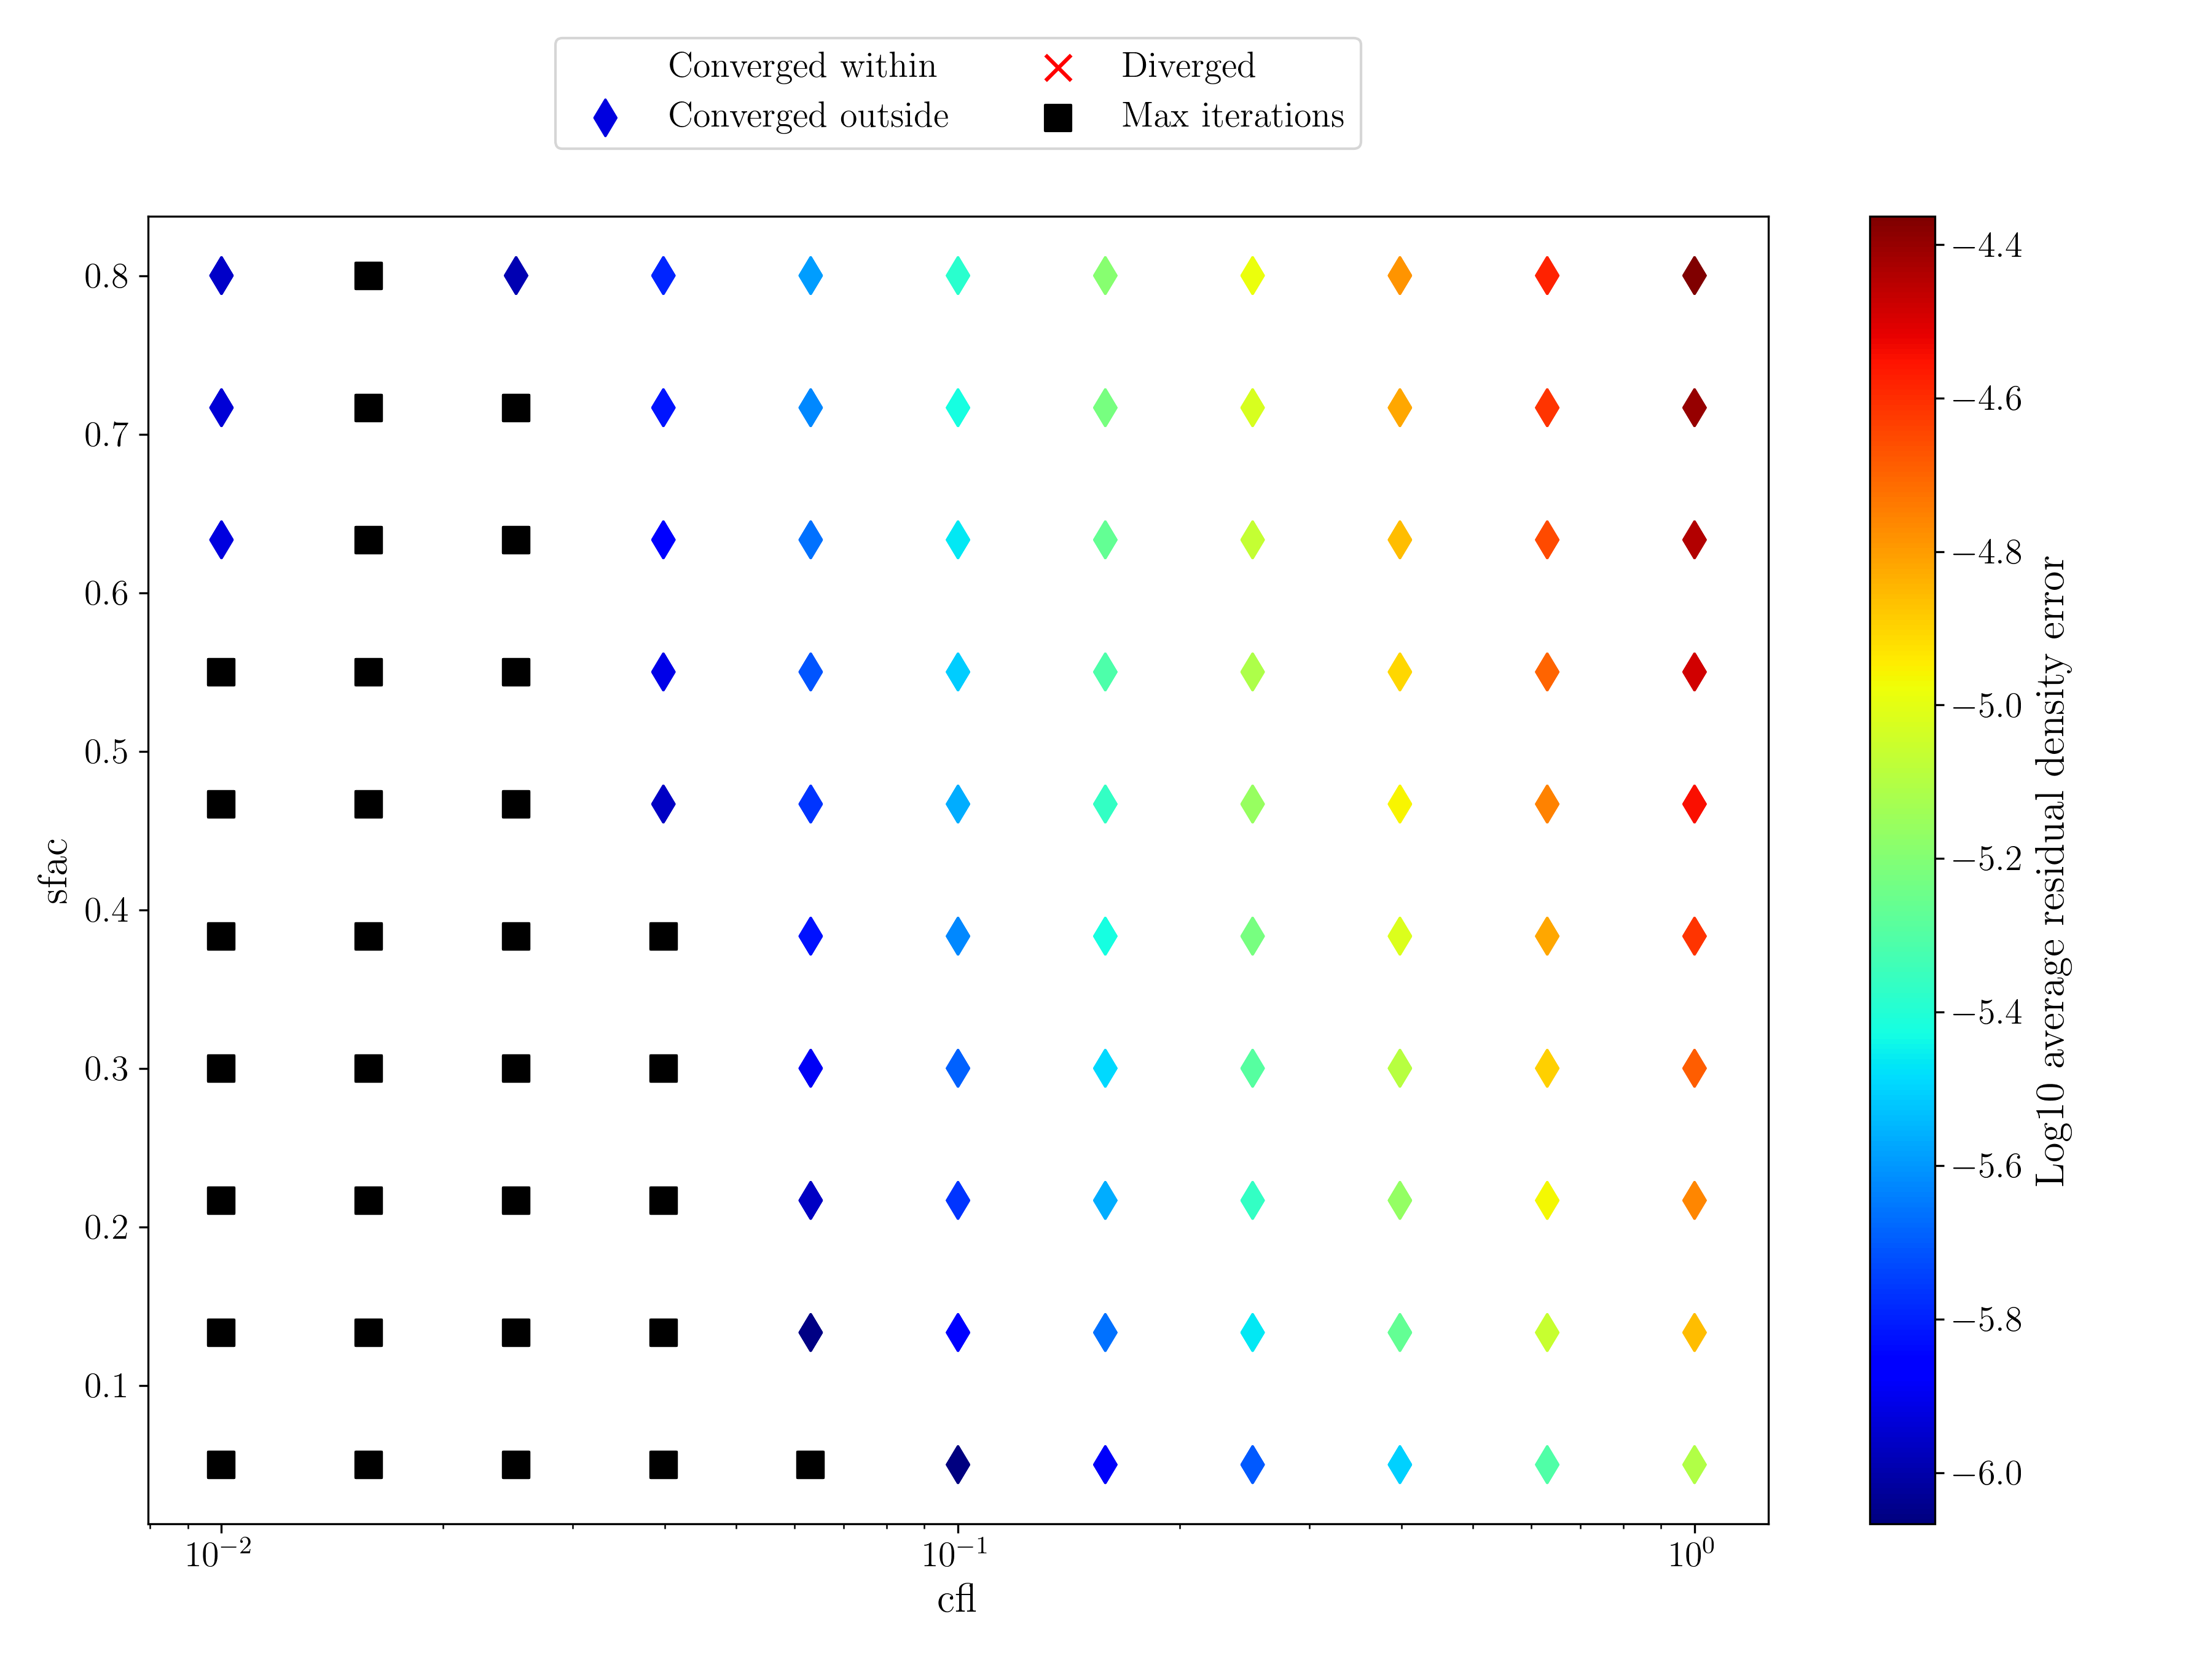
\includegraphics[width=0.7\textwidth]{figures/cfl_sfac_dro_avg.png}
    \caption{}
    \label{fig:cfl_sfac_dro_avg}
\end{figure}

\subsection{Effort vs Accuracy}

\begin{figure}[H]
    \begin{subfigure}{0.49\textwidth}
        \centering
        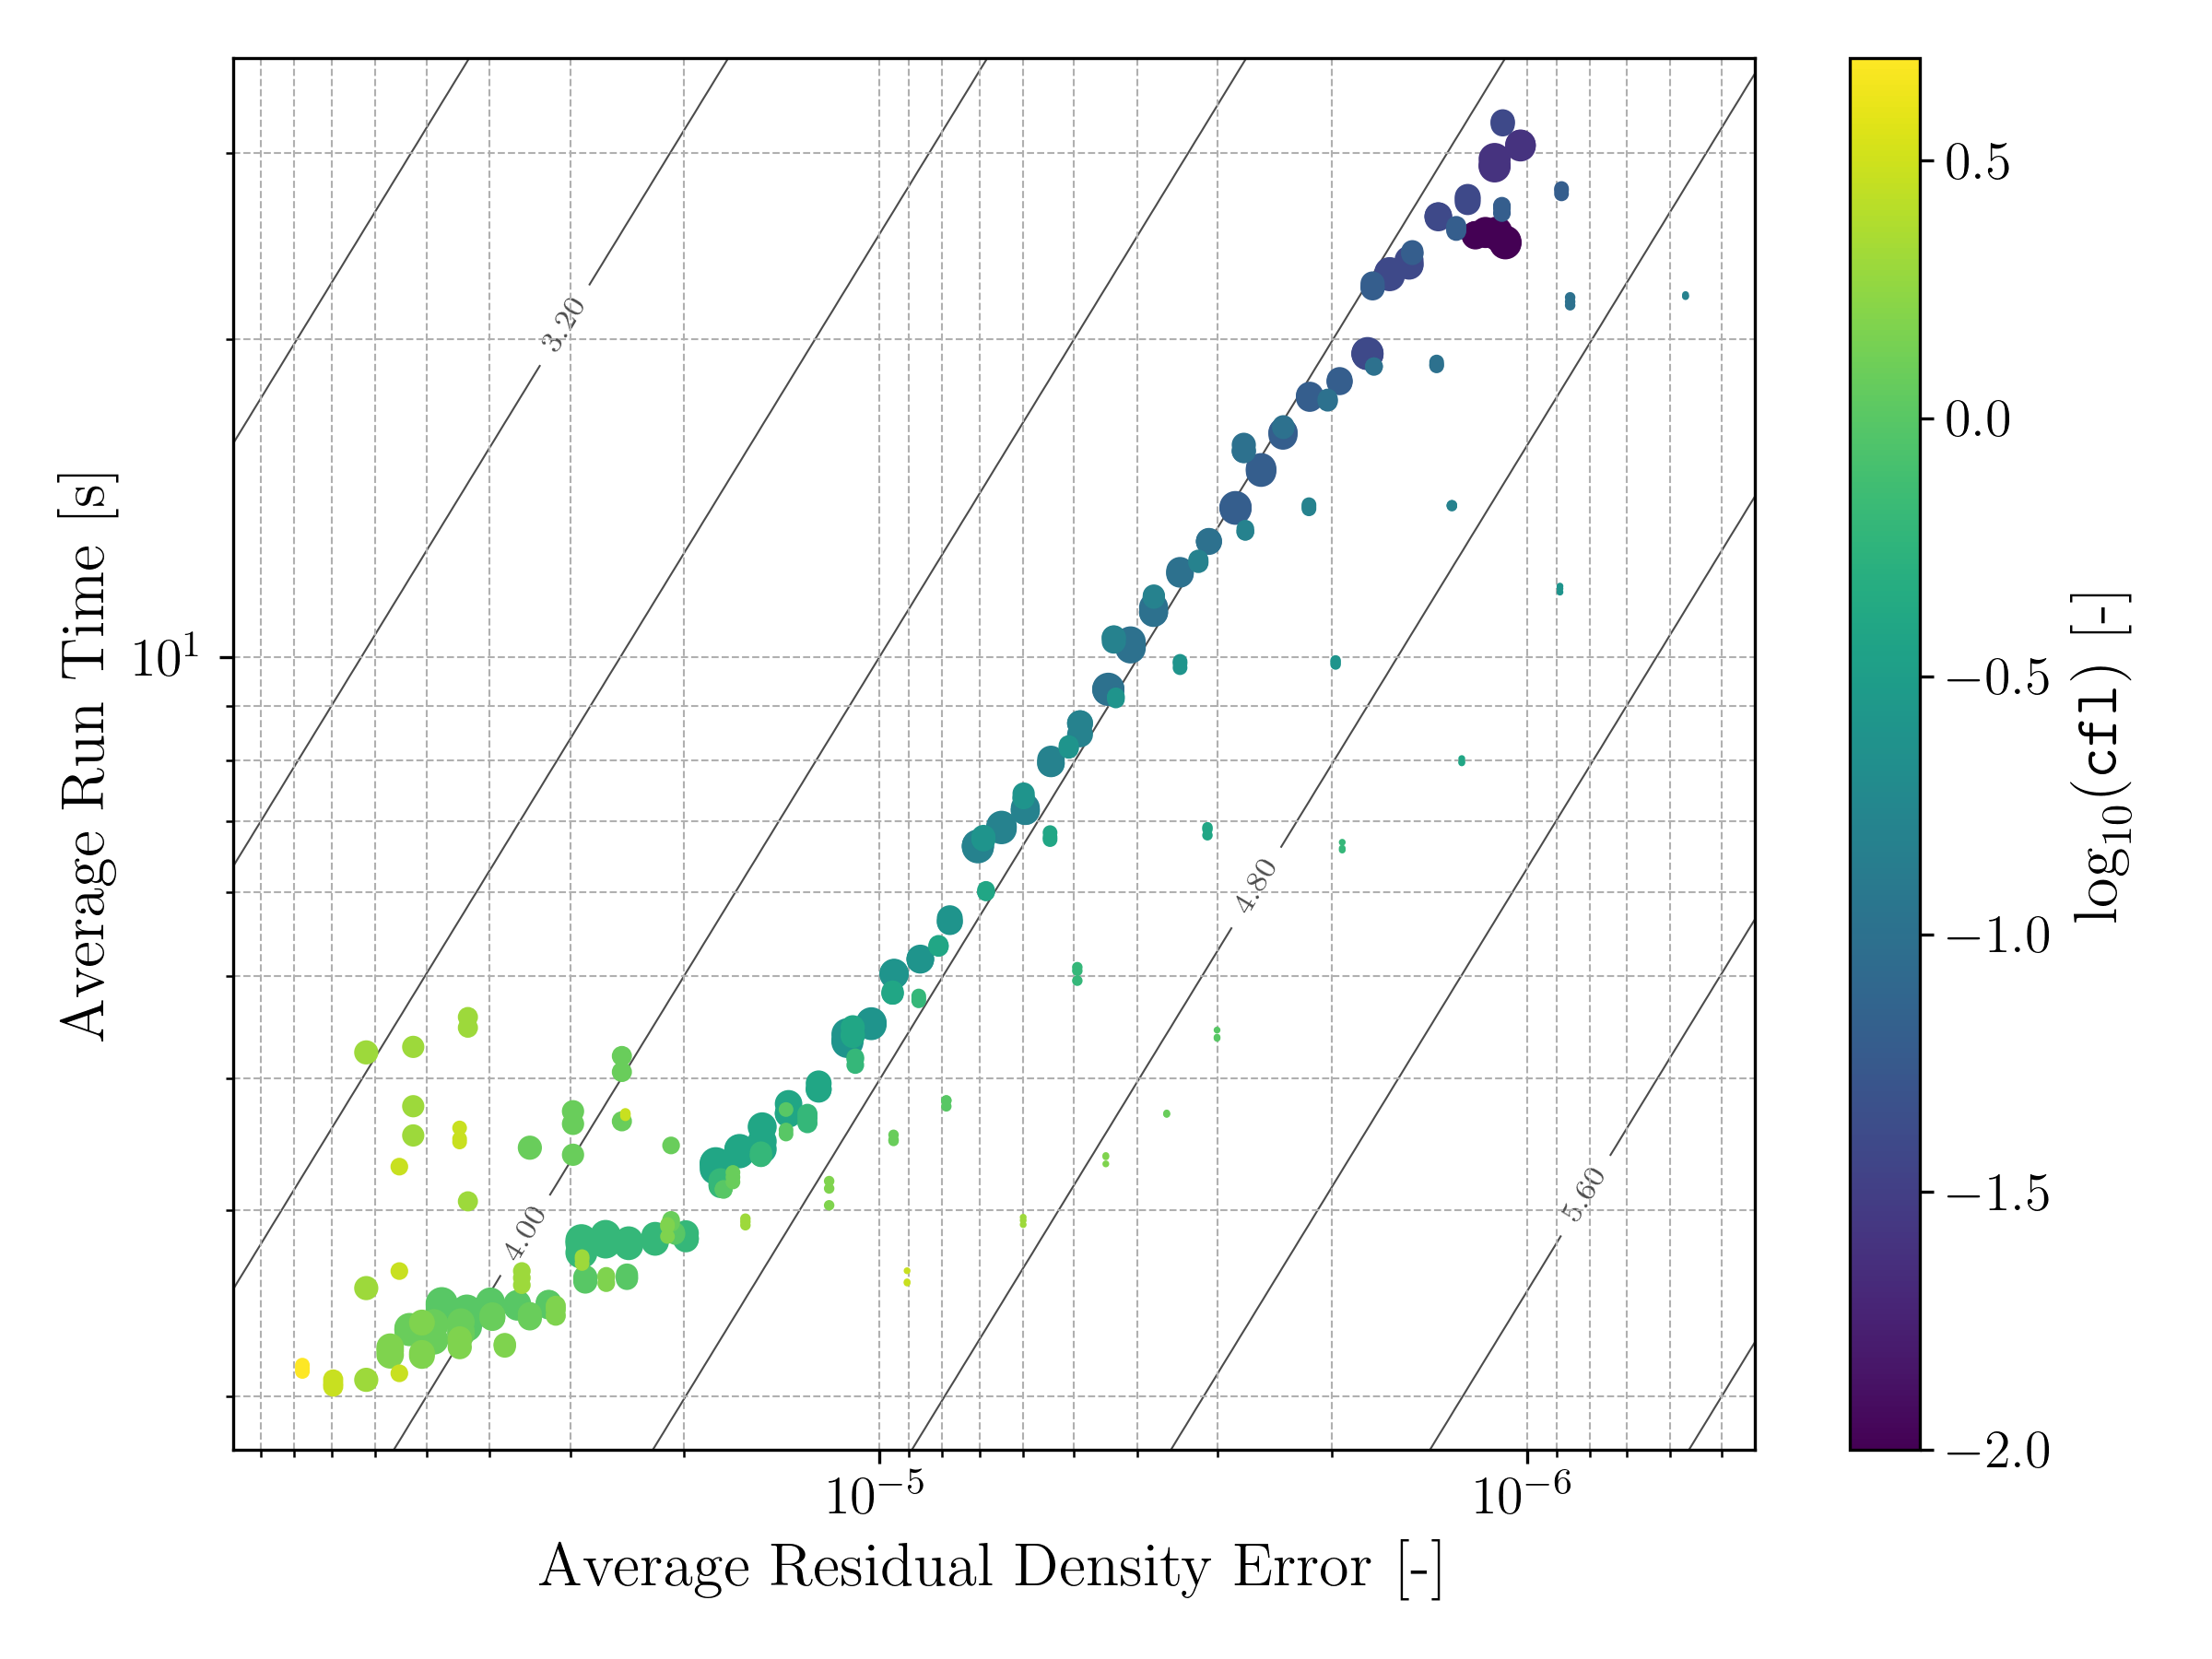
\includegraphics[width=0.99\textwidth]{figures/effort_vs_accuracy_cfl.png}
        \caption{Colour is $\log_{10}( \texttt{cfl})$ and size represents \texttt{sfac}.}
        \label{fig:effort_vs_accuracy_cfl}
    \end{subfigure}
    \begin{subfigure}{0.49\textwidth}
        \centering
        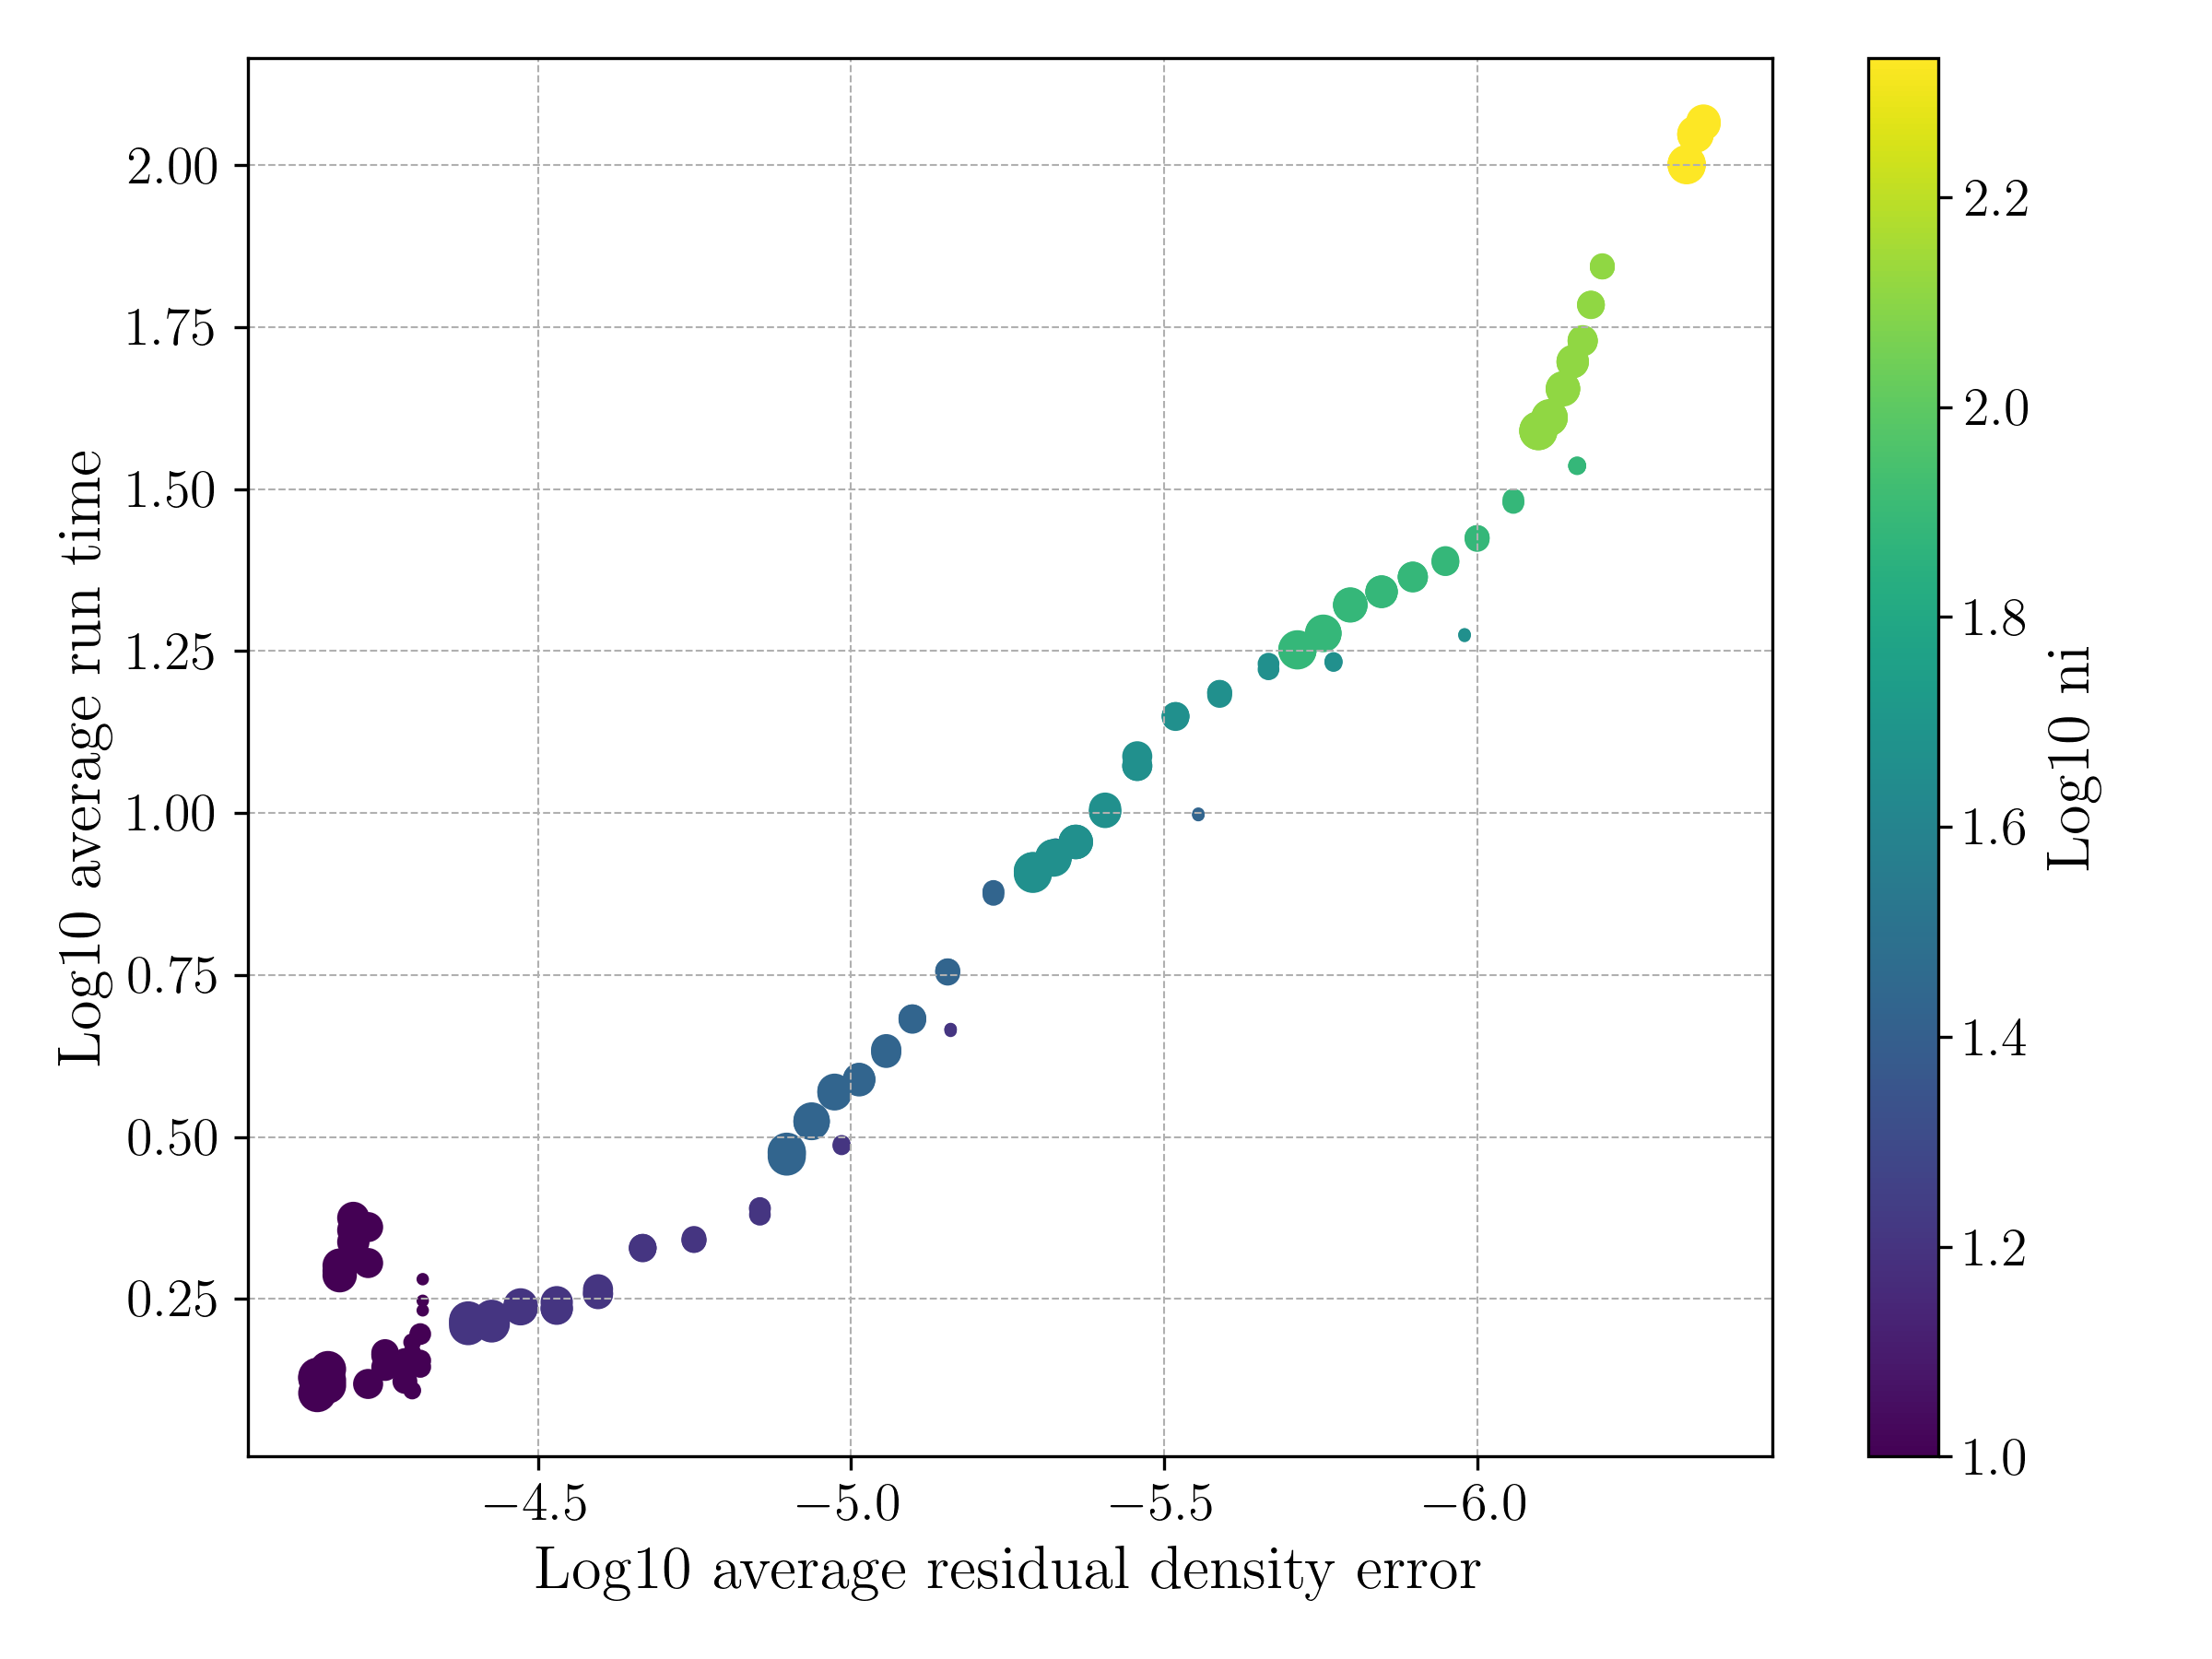
\includegraphics[width=0.99\textwidth]{figures/effort_vs_accuracy_ni.png}
        \caption{Colour is $\log_{10}( \texttt{ni})$ and size represents \texttt{sfac}.}
        \label{fig:effort_vs_accuracy_ni}
    \end{subfigure}
    \caption{Effort vs accuracy for bump case with varying parameters}
\end{figure}

\begin{figure}[H]
    \begin{subfigure}{0.49\textwidth}
        \centering
        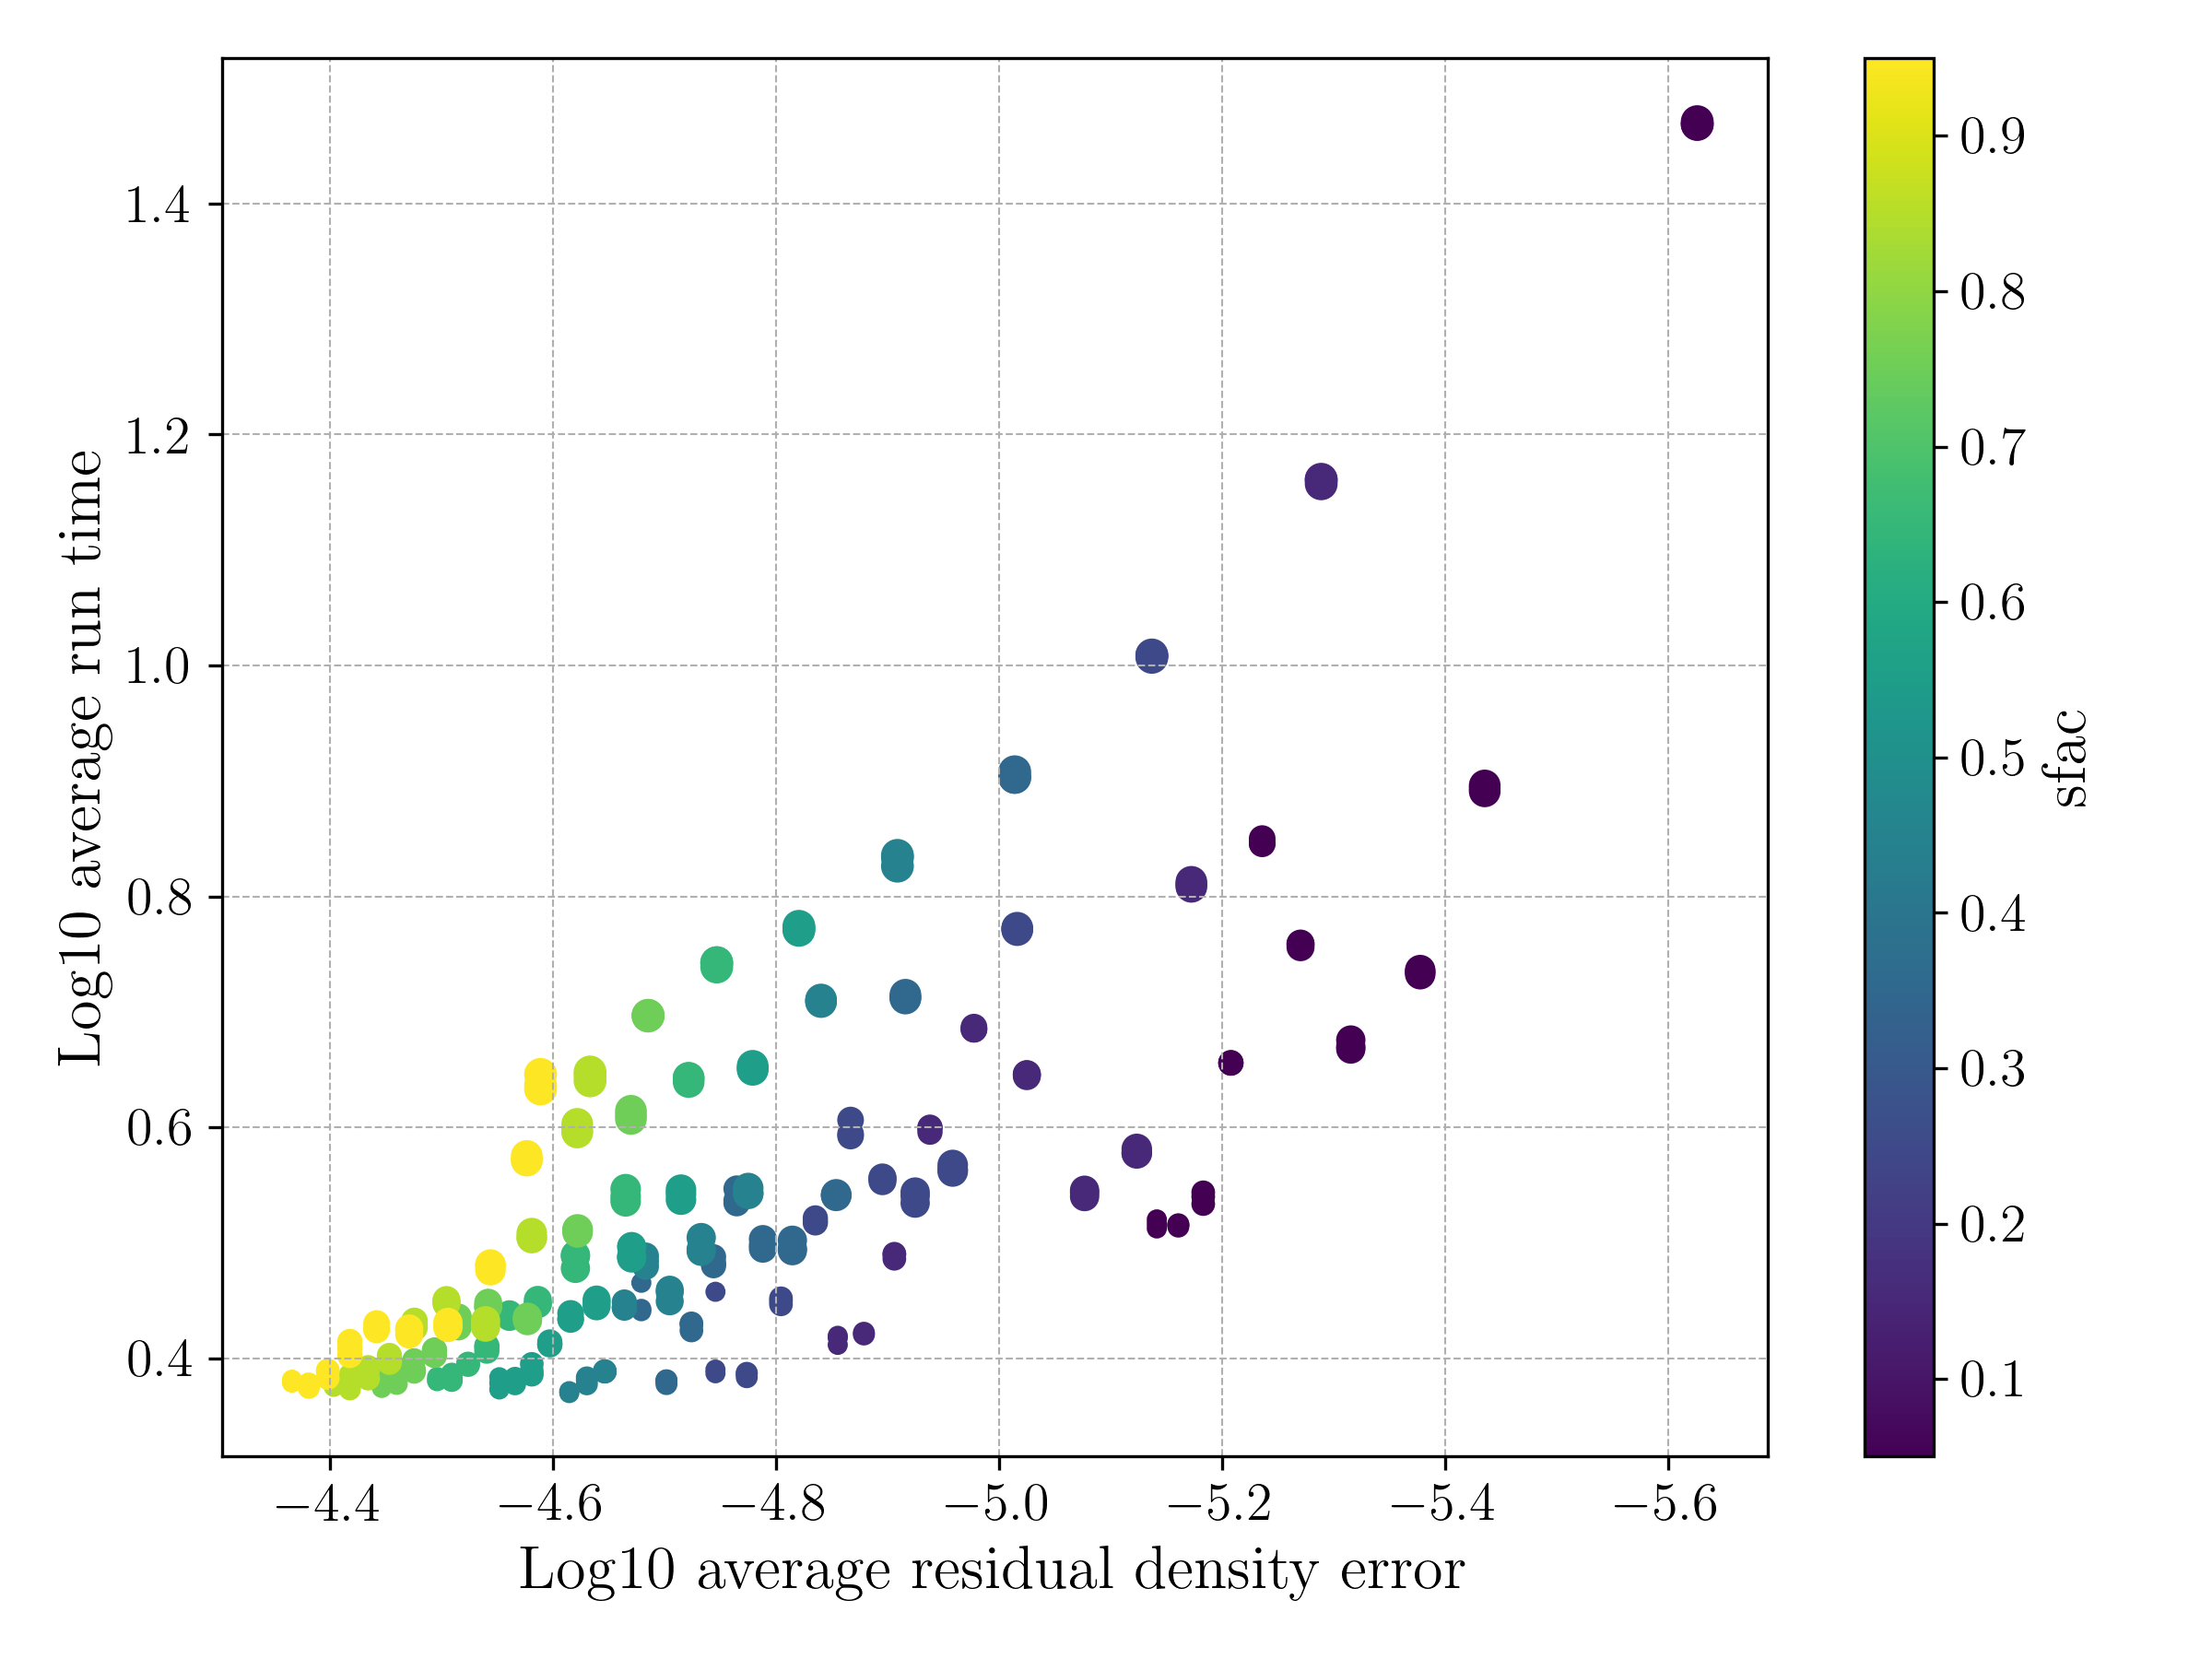
\includegraphics[width=0.99\textwidth]{figures/effort_vs_accuracy_sfac_res.png}
        \caption{Colour is \texttt{sfac} and size represents \texttt{sfac\_res}.}
        \label{fig:effort_vs_accuracy_sfac_res}
    \end{subfigure}
    \begin{subfigure}{0.49\textwidth}
        \centering
        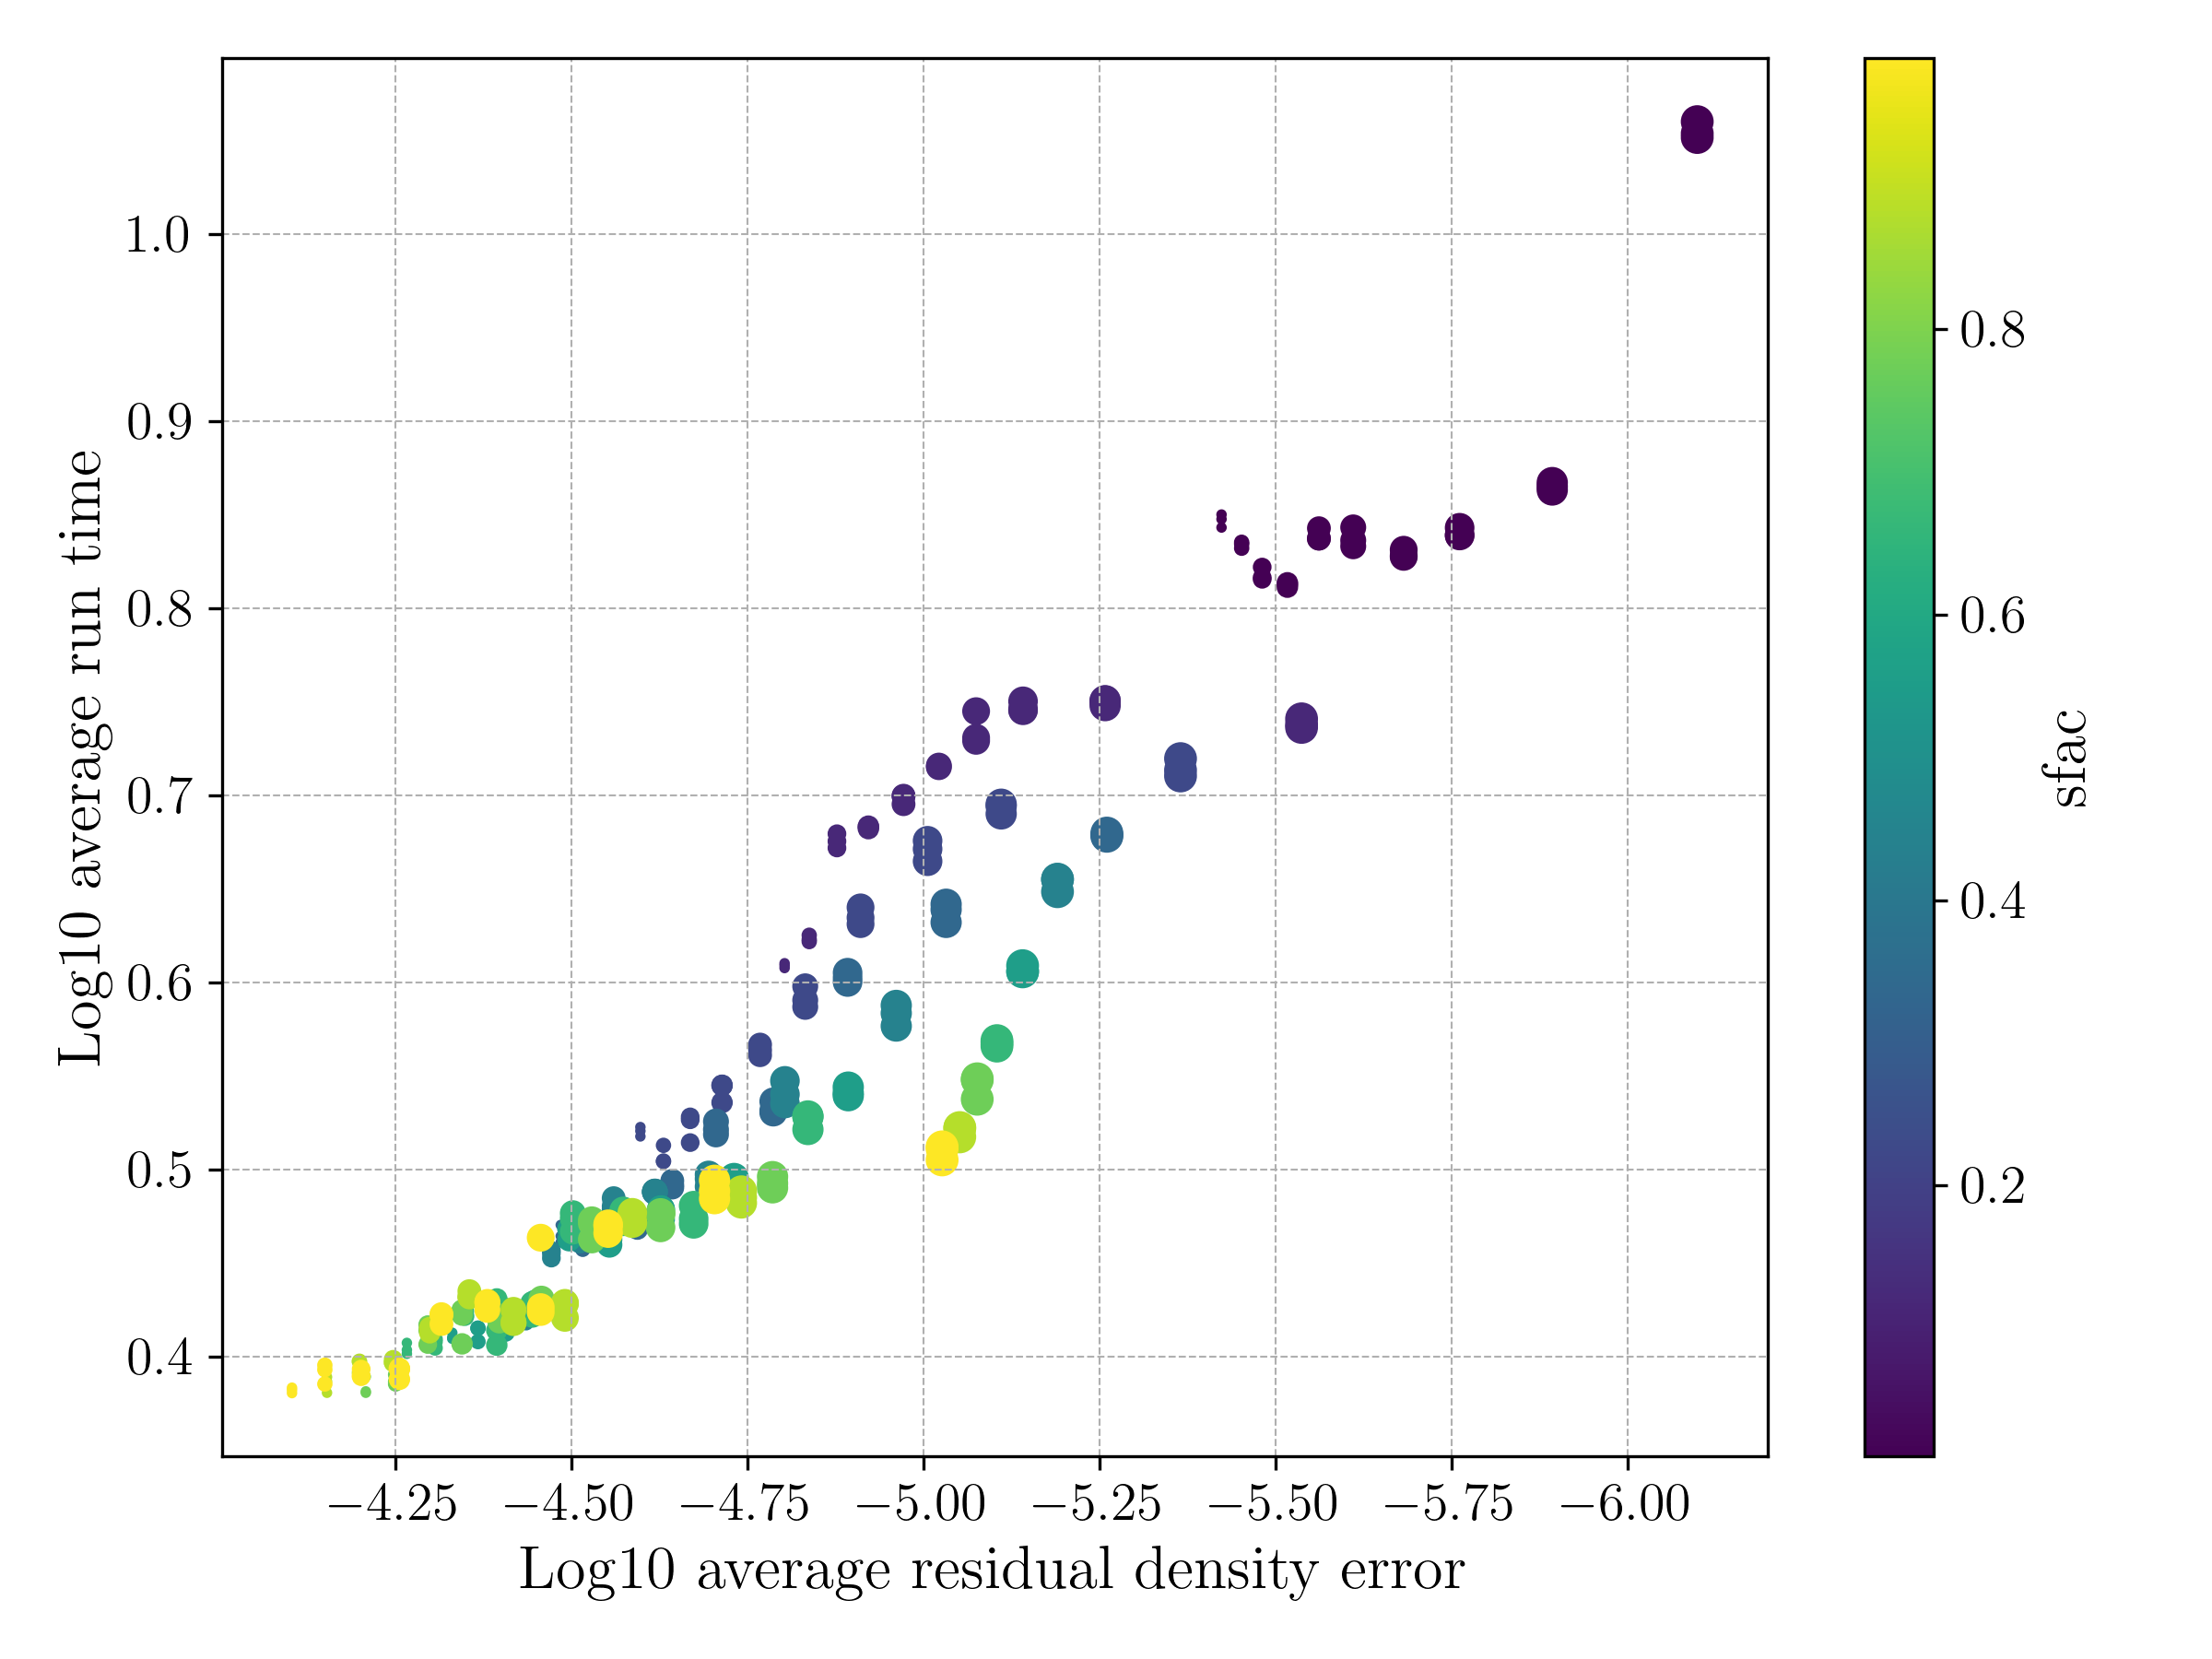
\includegraphics[width=0.99\textwidth]{figures/effort_vs_accuracy_fcorr.png}
        \caption{Colour is \texttt{sfac} and size represents \texttt{fcorr}.}
        \label{fig:effort_vs_accuracy_fcorr}
    \end{subfigure}
    \caption{Effort vs accuracy for bump case with varying parameters. Contours are $FM$.}
\end{figure}

\subsection{NACA airfoils}

\begin{figure}[H]
    \centering
    \begin{subfigure}{0.49\textwidth}
        \centering
        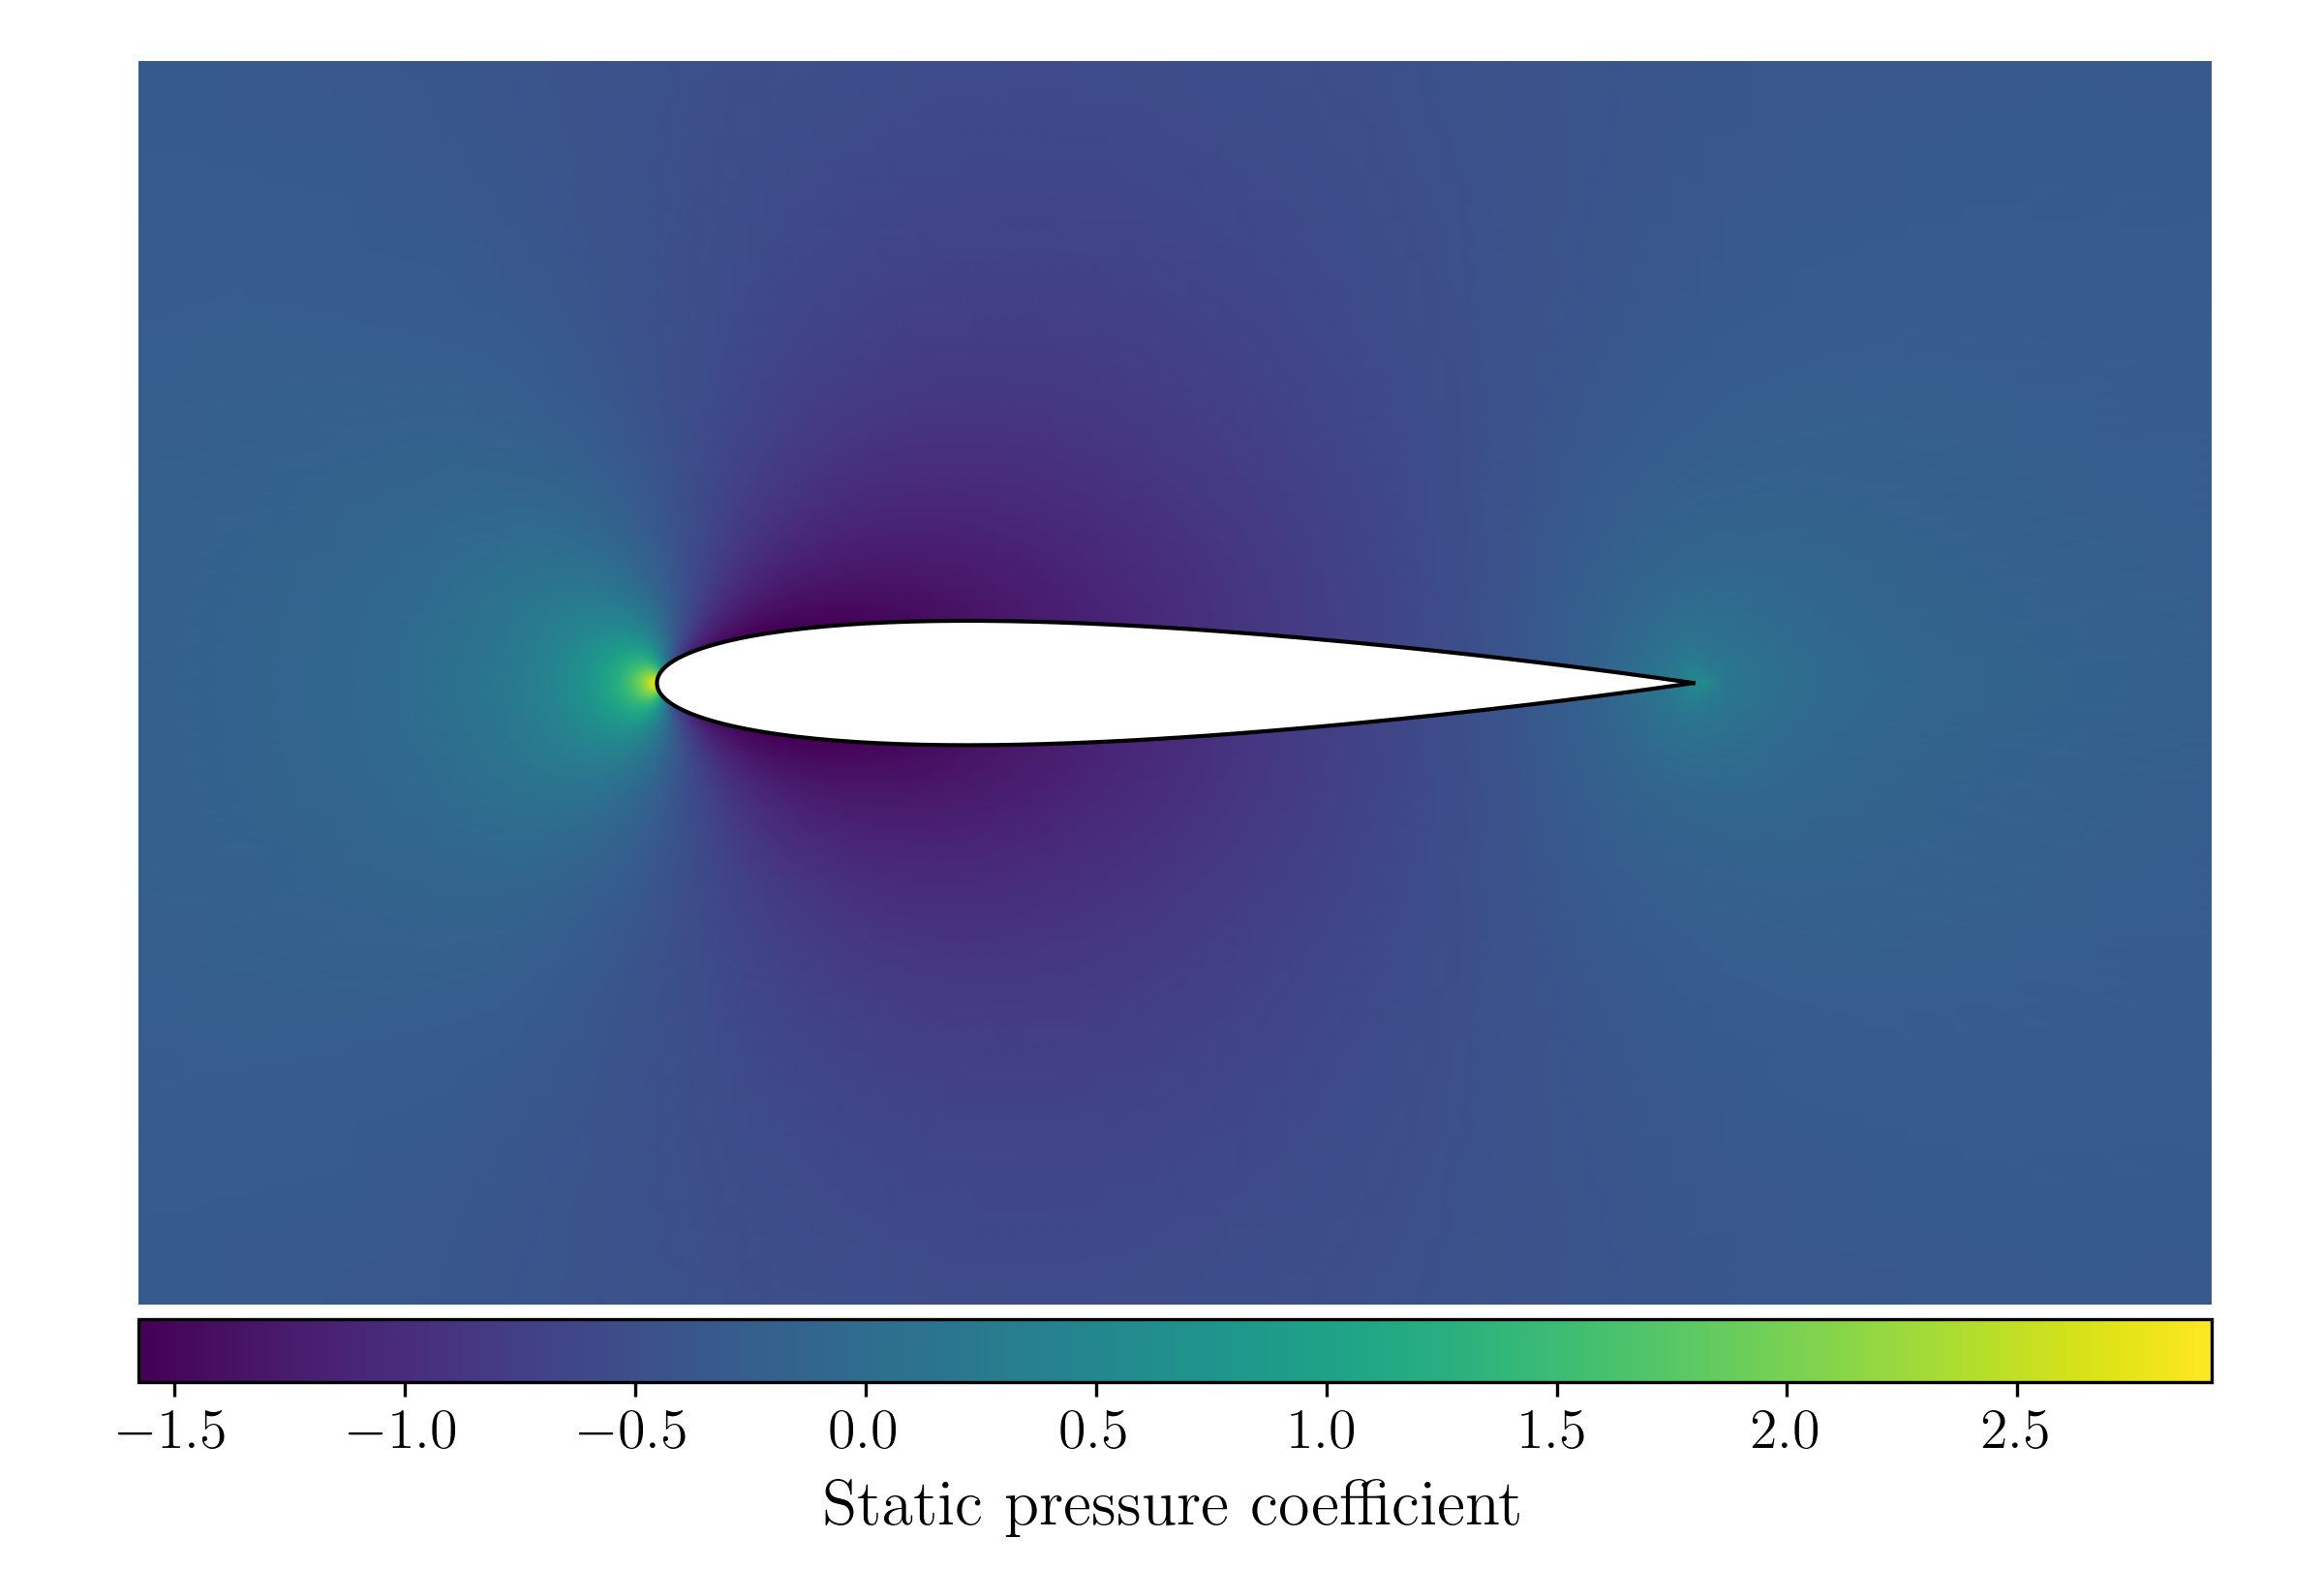
\includegraphics[width=0.99\textwidth]{figures/naca0012_cp.png}
        \caption{}
        \label{fig:naca0012_cp}
    \end{subfigure}
    \begin{subfigure}{0.49\textwidth}
        \centering
        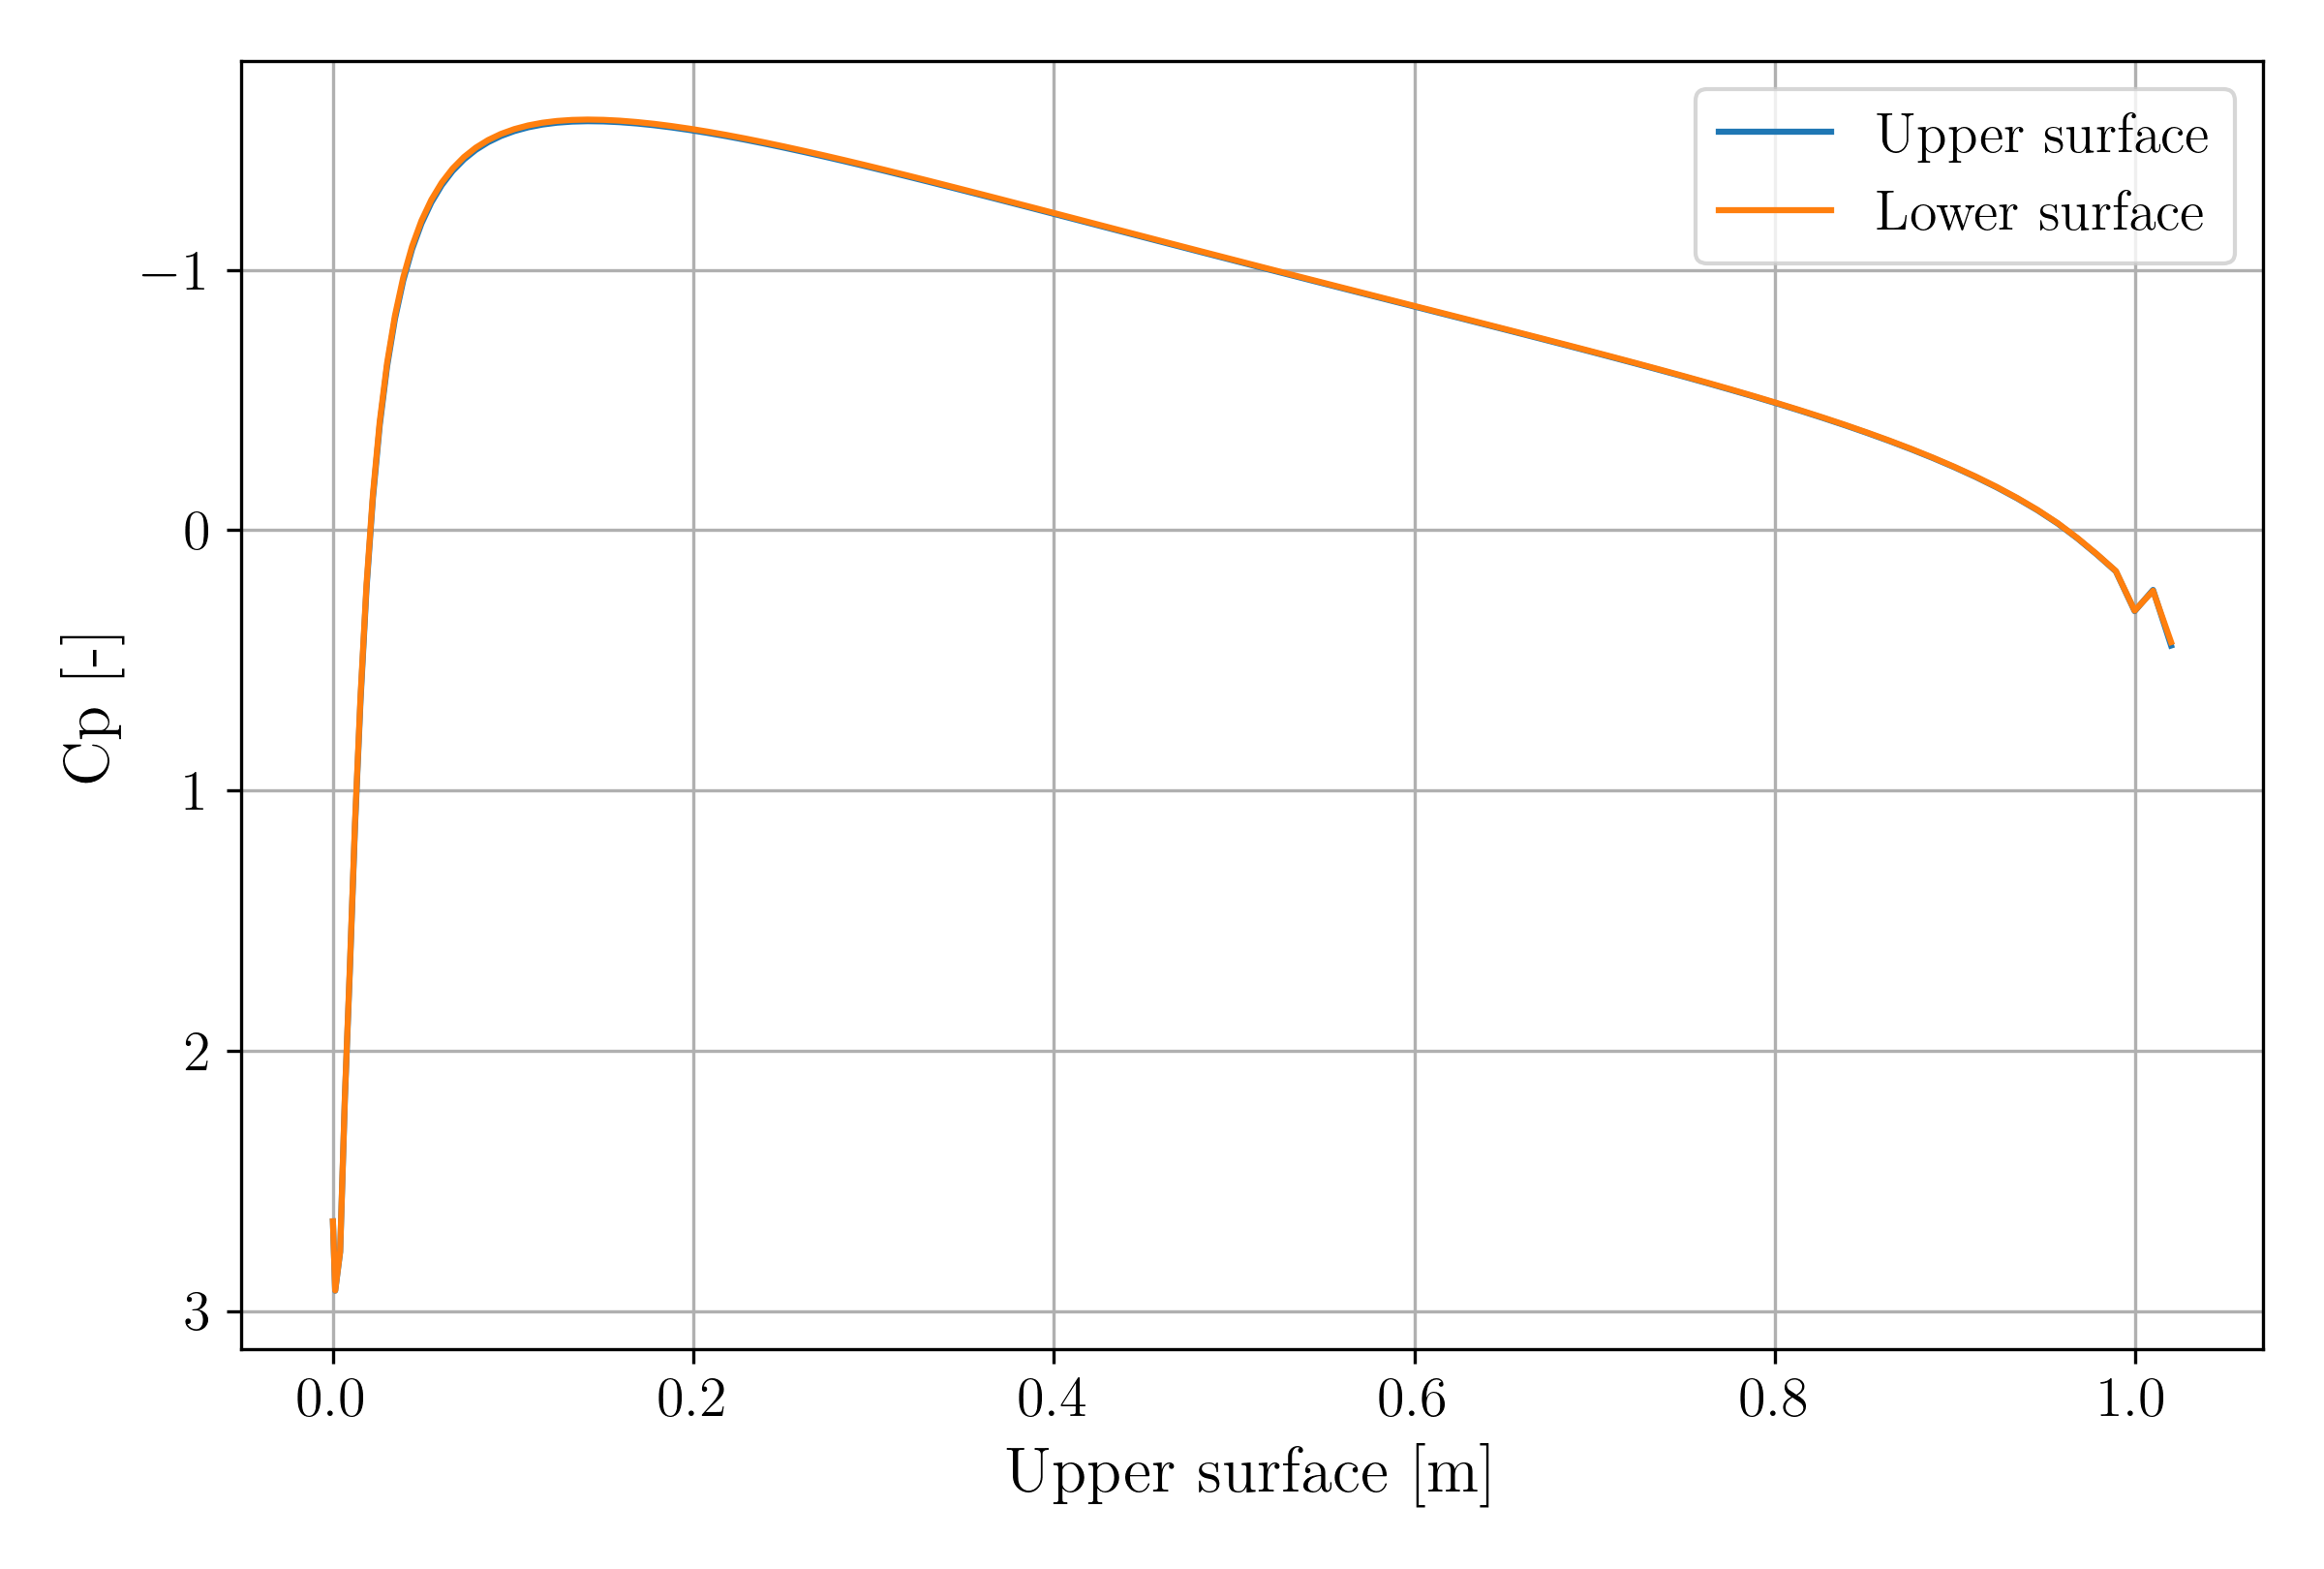
\includegraphics[width=0.99\textwidth]{figures/naca0012_surface_cp.png}
        \caption{}
        \label{fig:naca0012_mach}
    \end{subfigure}
    \caption{NACA0012 test case results}
\end{figure}

\begin{figure}[H]
    \centering
    \begin{subfigure}{0.49\textwidth}
        \centering
        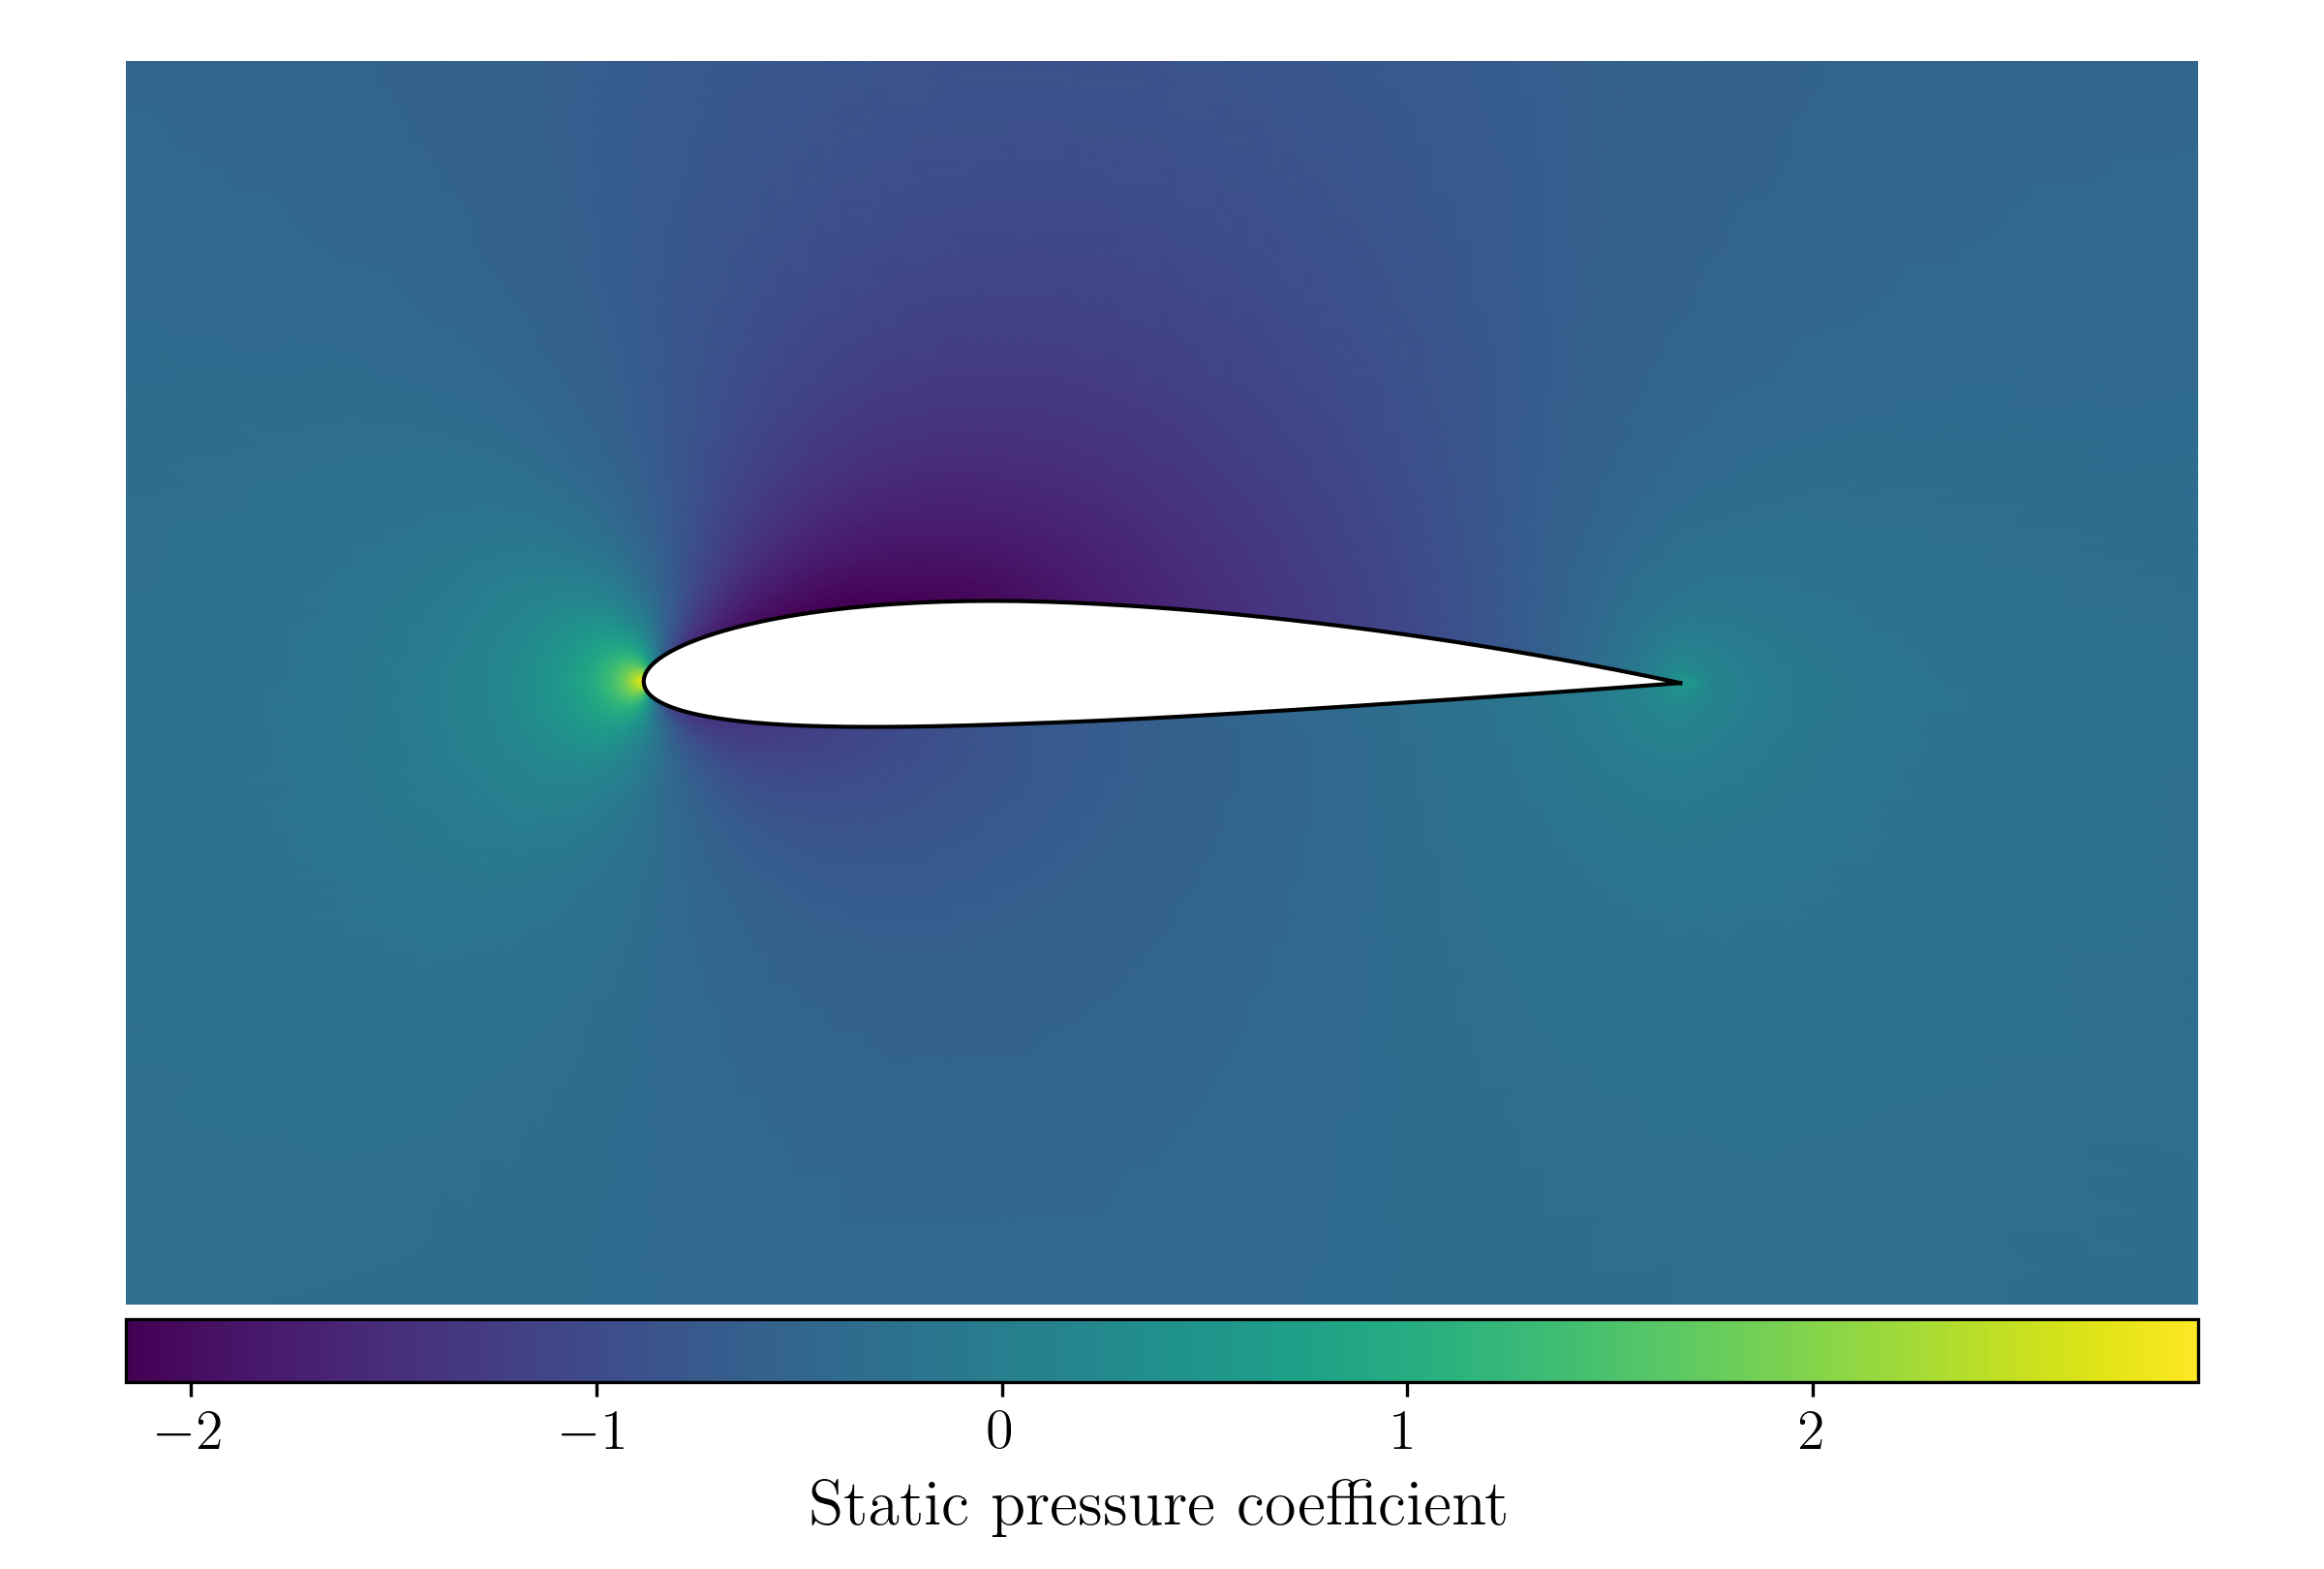
\includegraphics[width=0.99\textwidth]{figures/naca2412_cp.png}
        \caption{}
        \label{fig:naca2412_cp}
    \end{subfigure}
    \begin{subfigure}{0.49\textwidth}
        \centering
        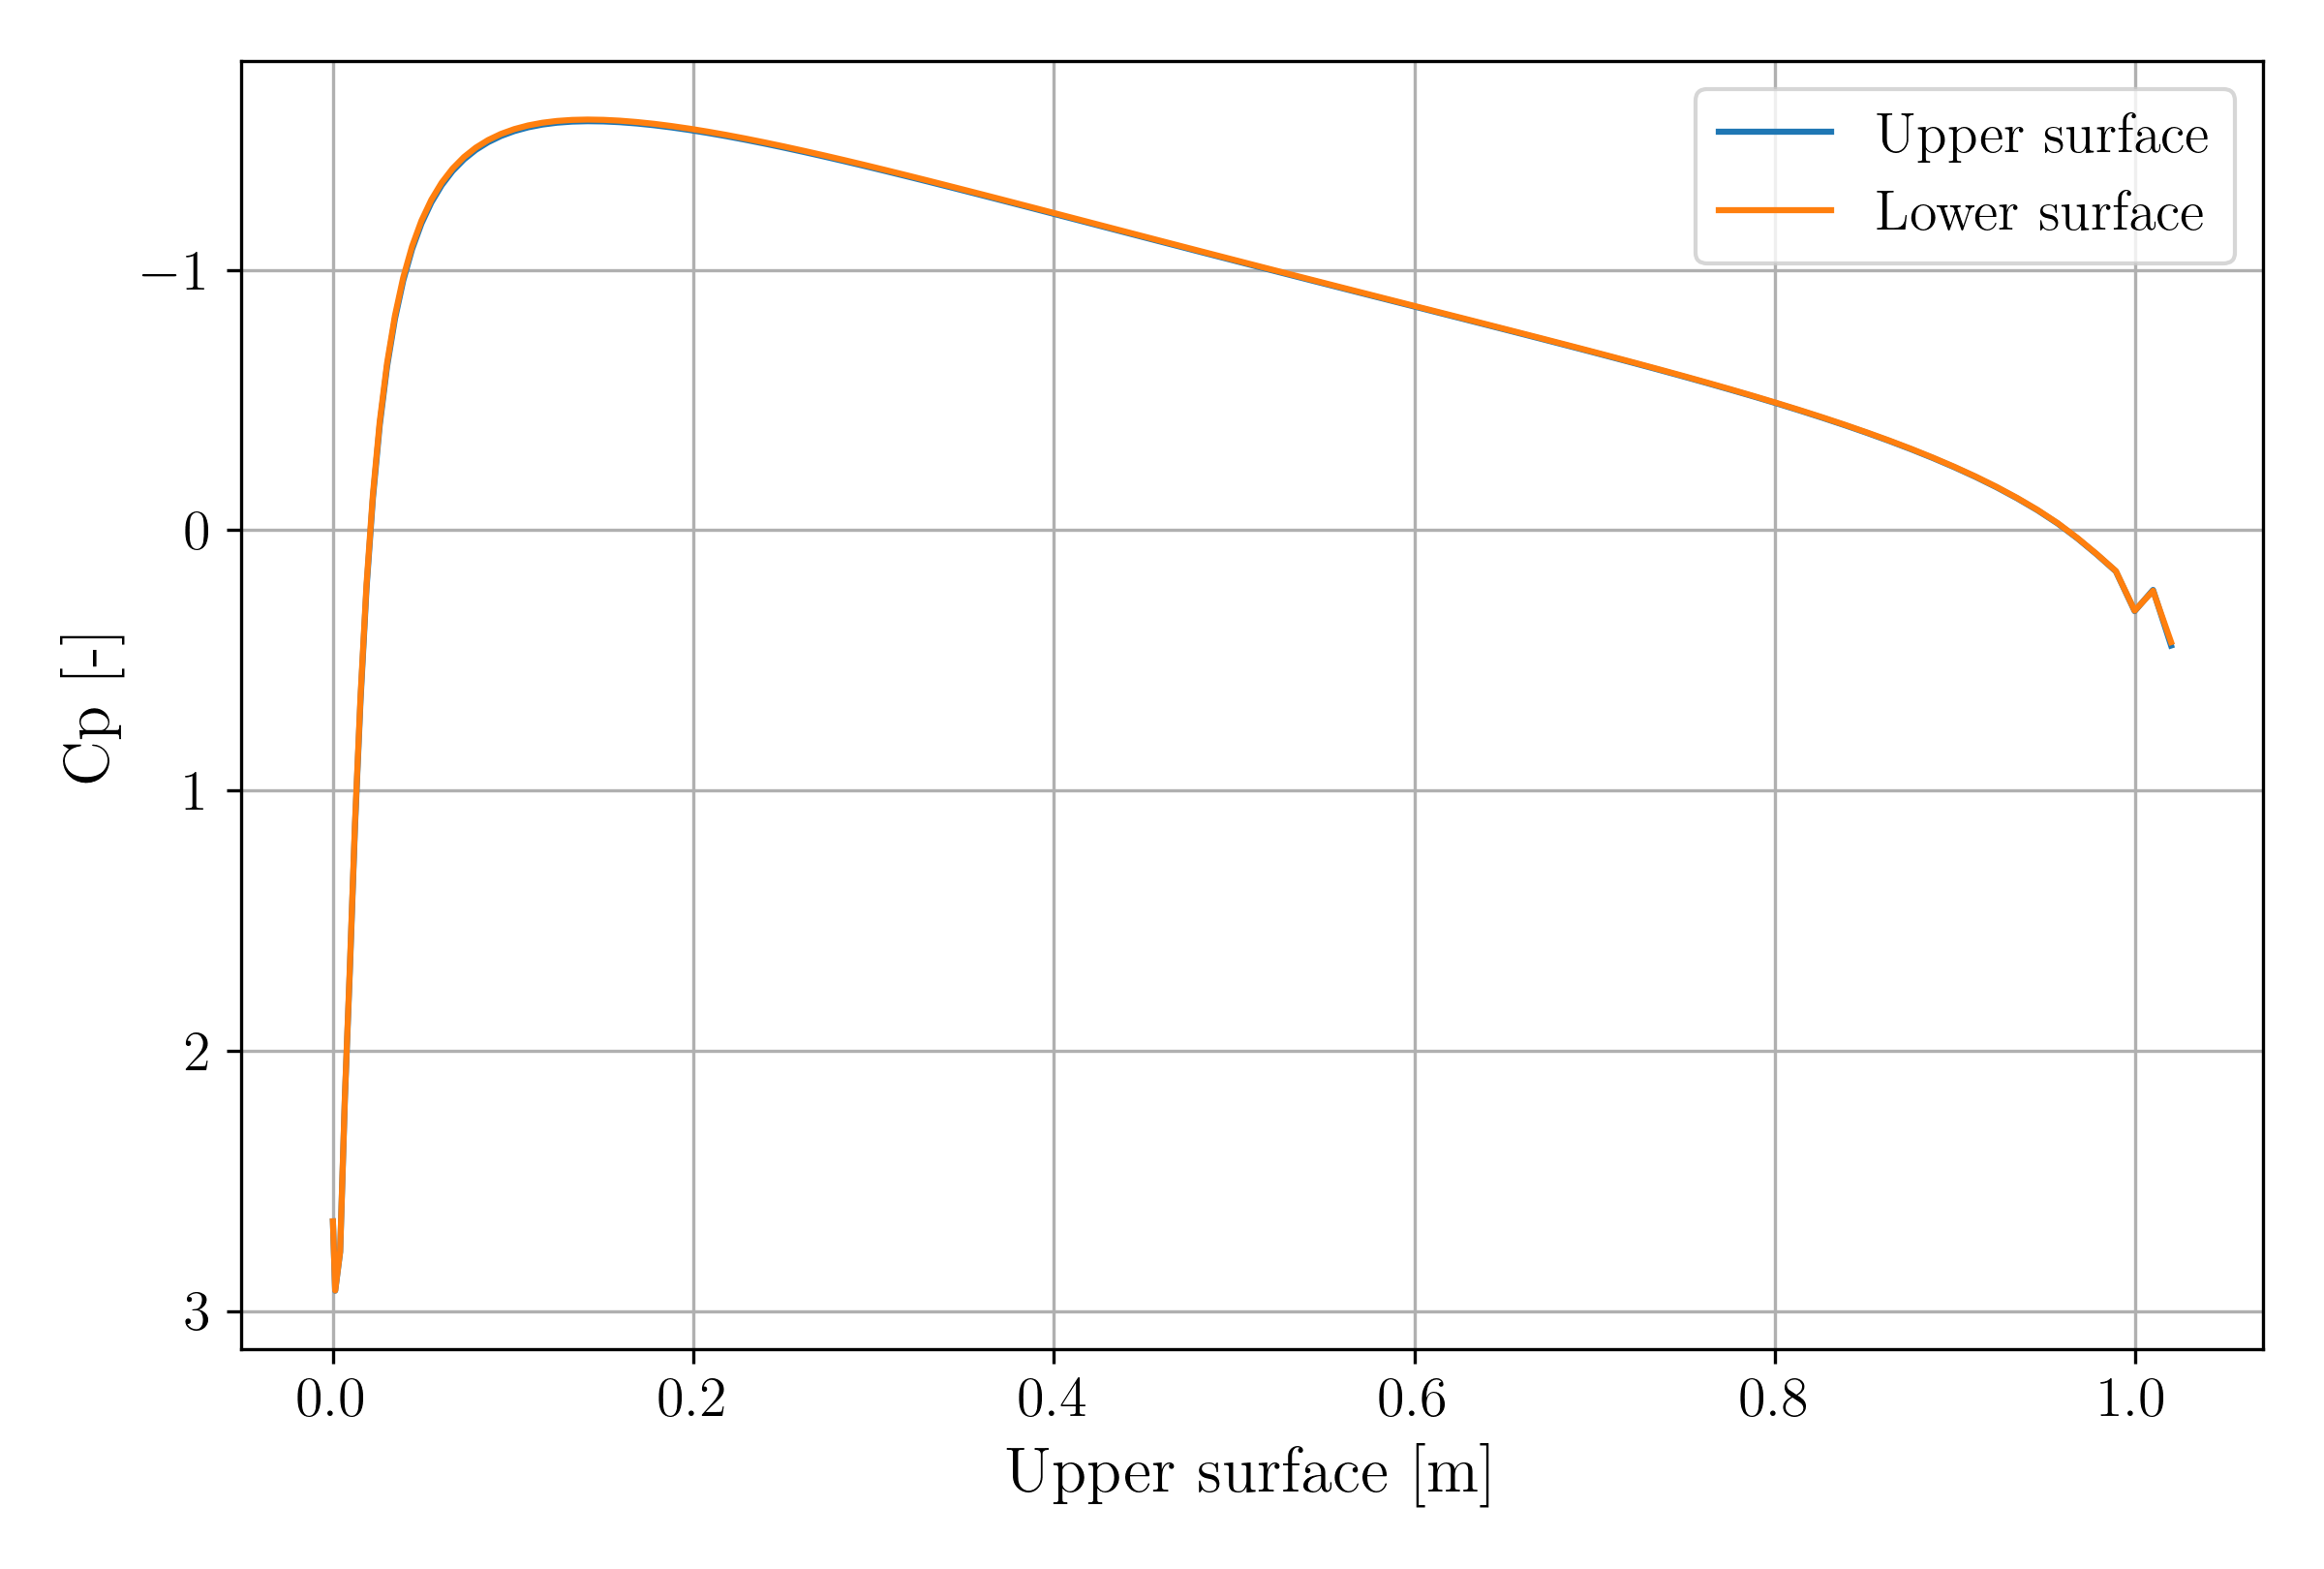
\includegraphics[width=0.99\textwidth]{figures/naca0012_surface_cp.png}
        \caption{}
        \label{fig:naca2412_mach}
    \end{subfigure}
    \caption{NACA2412 test case results}
\end{figure}

\begin{figure}[H]
    \centering
    \begin{subfigure}{0.49\textwidth}
        \centering
        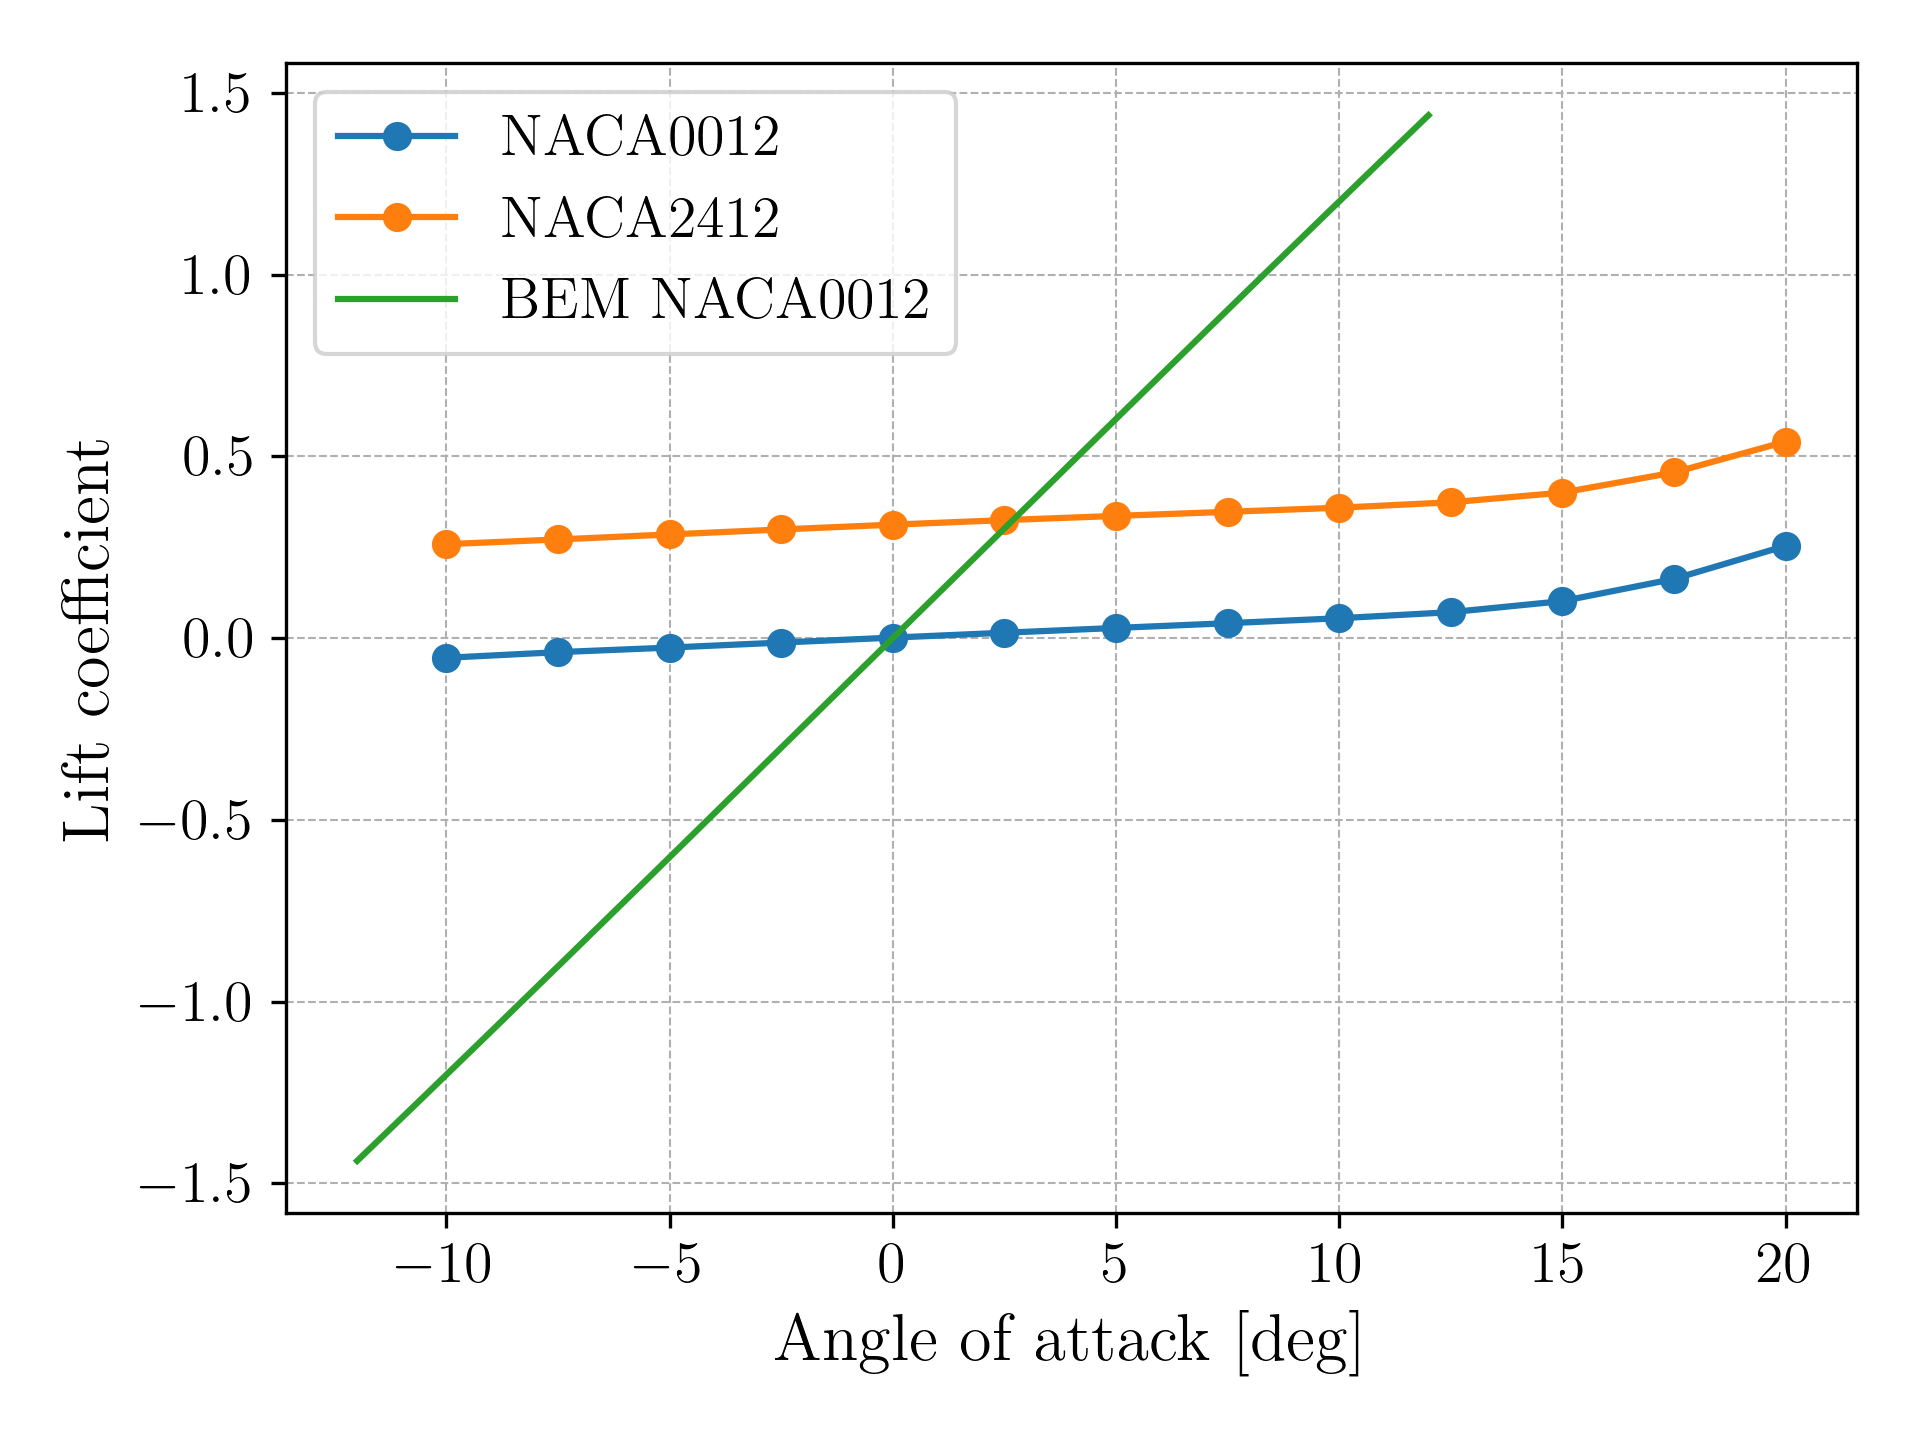
\includegraphics[width=0.99\textwidth]{figures/cl_alpha.png}
        \caption{}
        \label{fig:cl_alpha}
    \end{subfigure}
    \begin{subfigure}{0.49\textwidth}
        \centering
        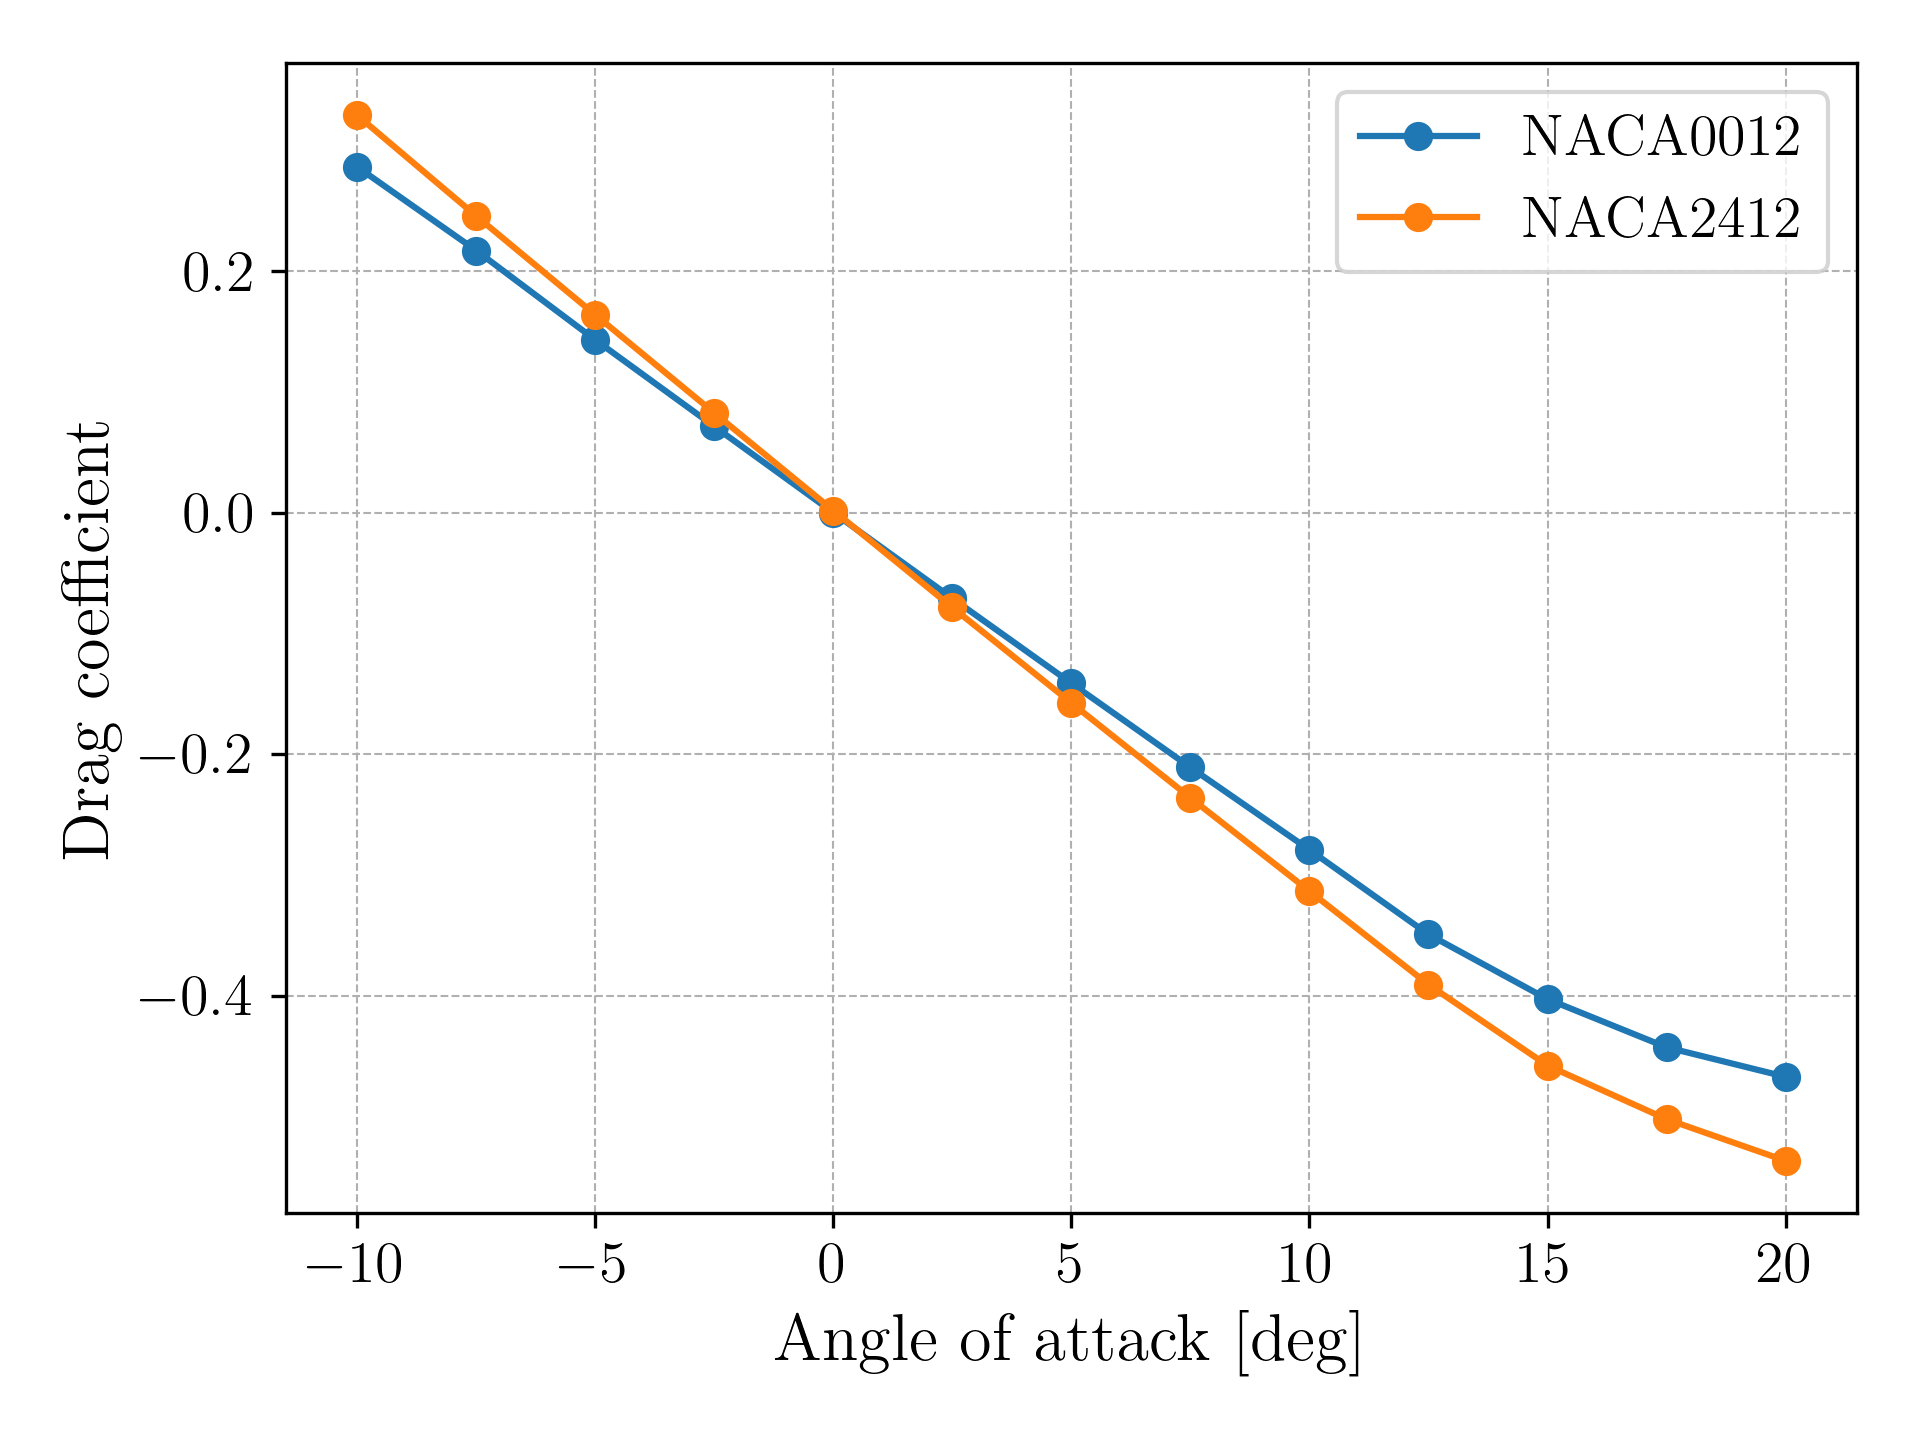
\includegraphics[width=0.99\textwidth]{figures/cd_alpha.png}
        \caption{}
        \label{fig:cd_alpha}
    \end{subfigure}
    \caption{NACA2412 test case results}
\end{figure}

\subsection{Turbine}

\begin{figure}[H]
    \centering
    \begin{subfigure}{0.44\textwidth}
        \centering
        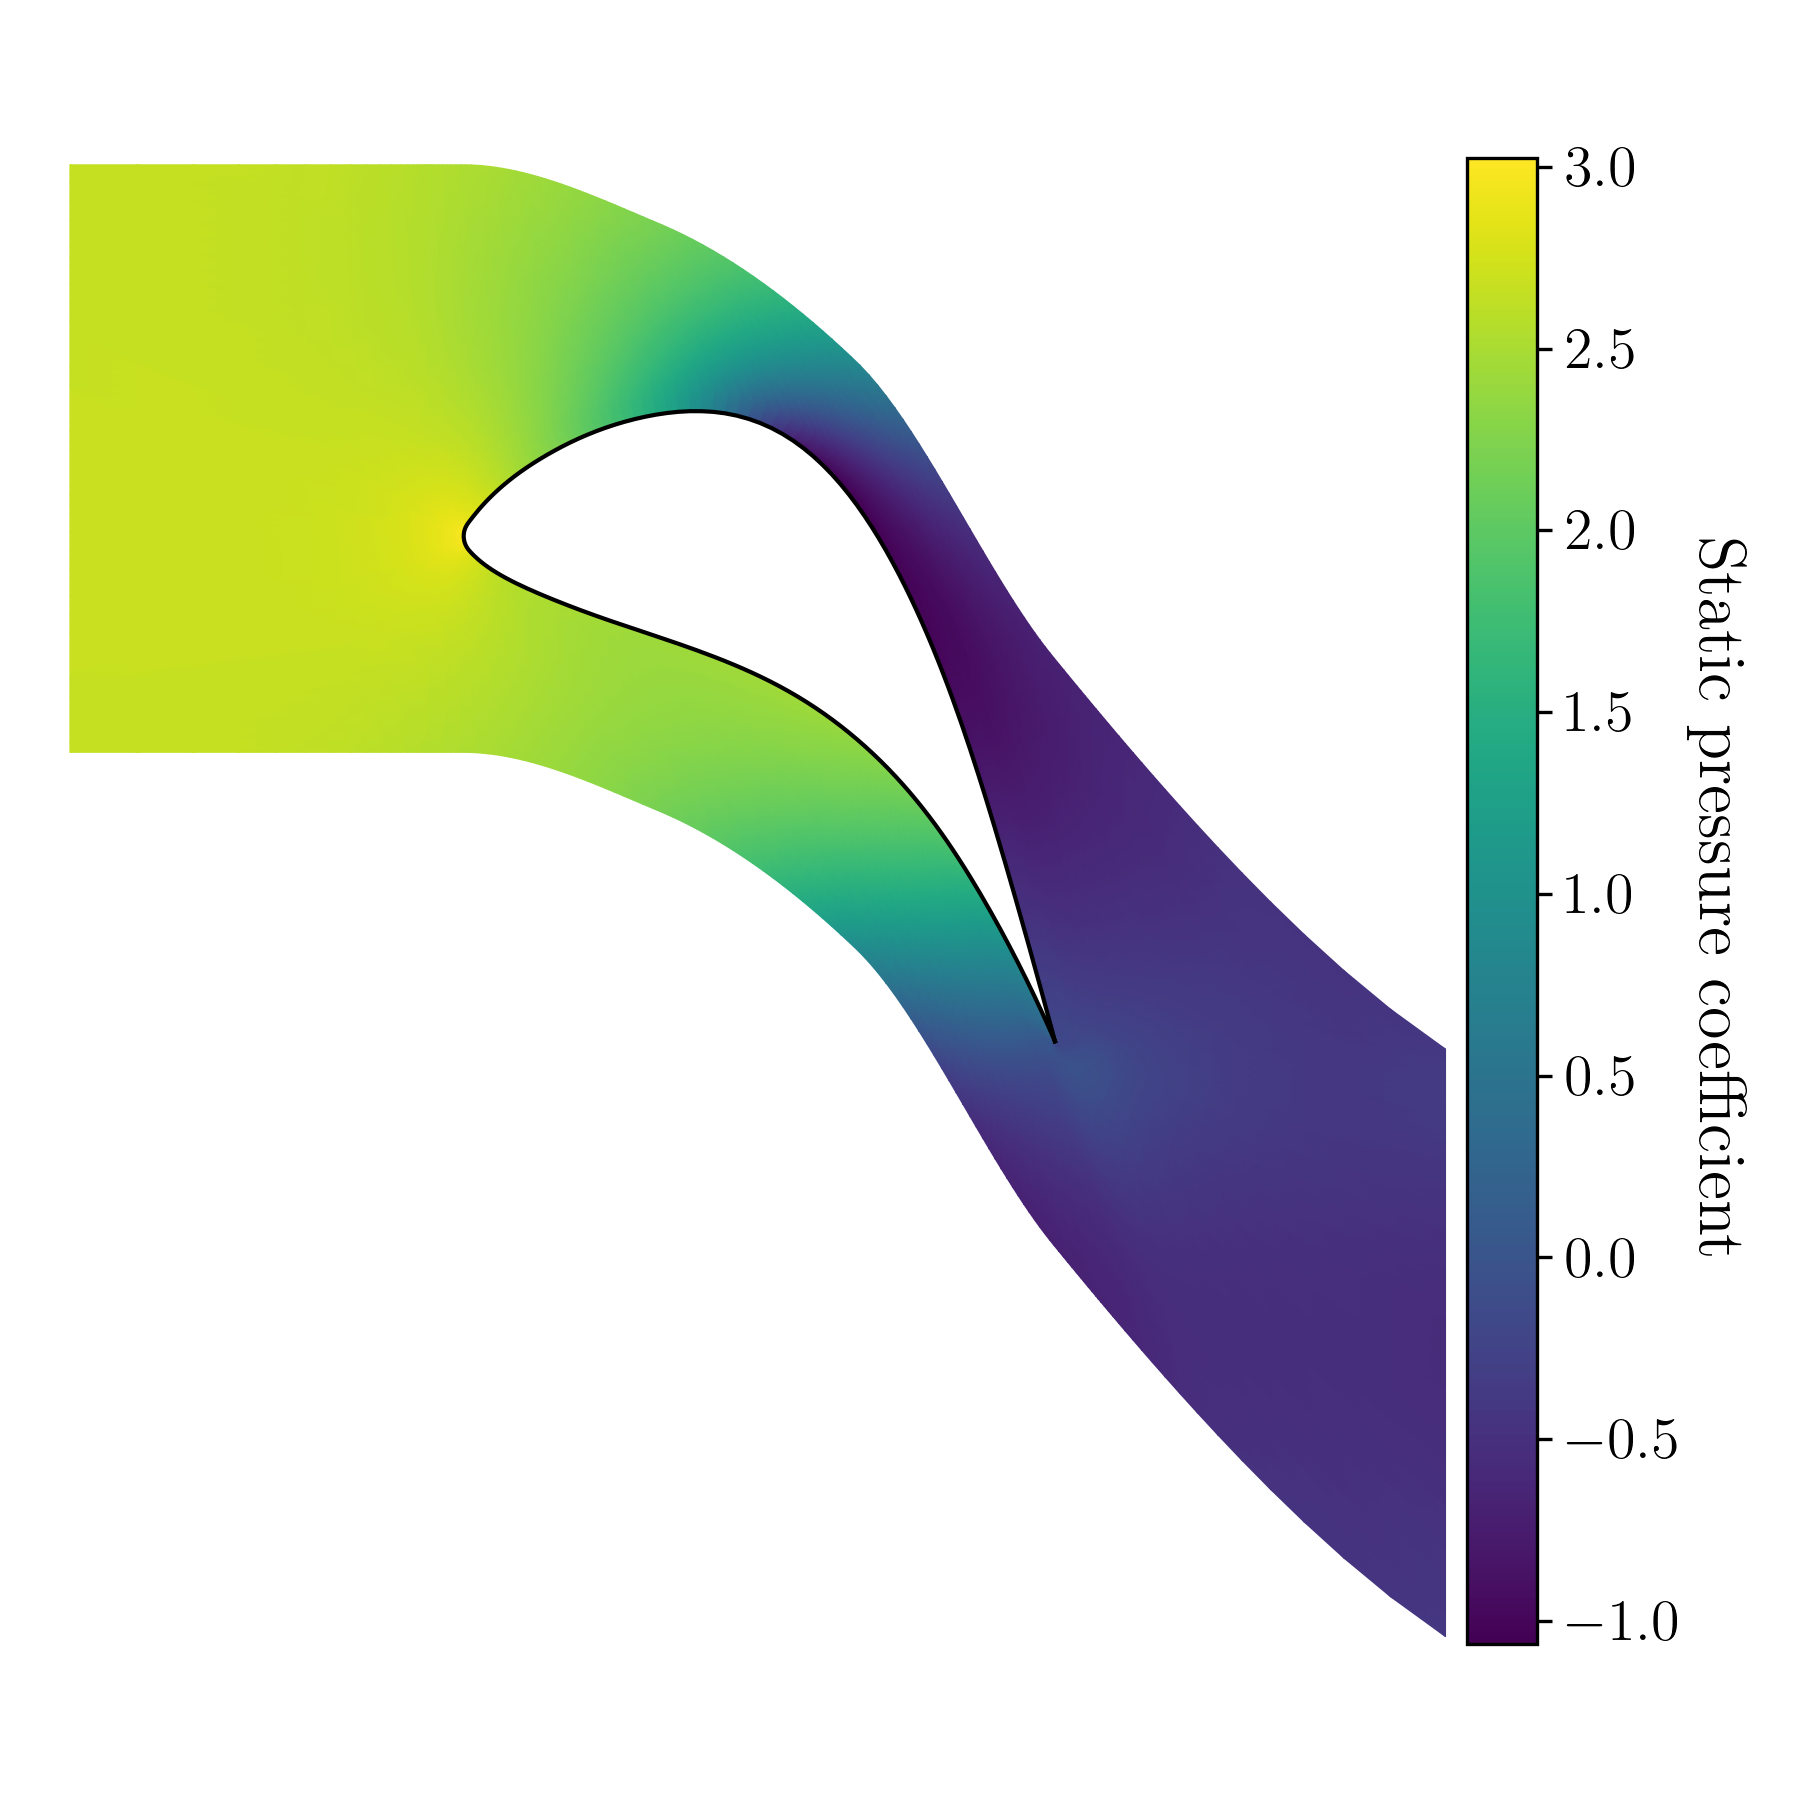
\includegraphics[width=0.99\textwidth]{figures/turbine_c_cp.png}
        \caption{}
        \label{fig:turbine_c_cp}
    \end{subfigure}
    \begin{subfigure}{0.55\textwidth}
        \centering
        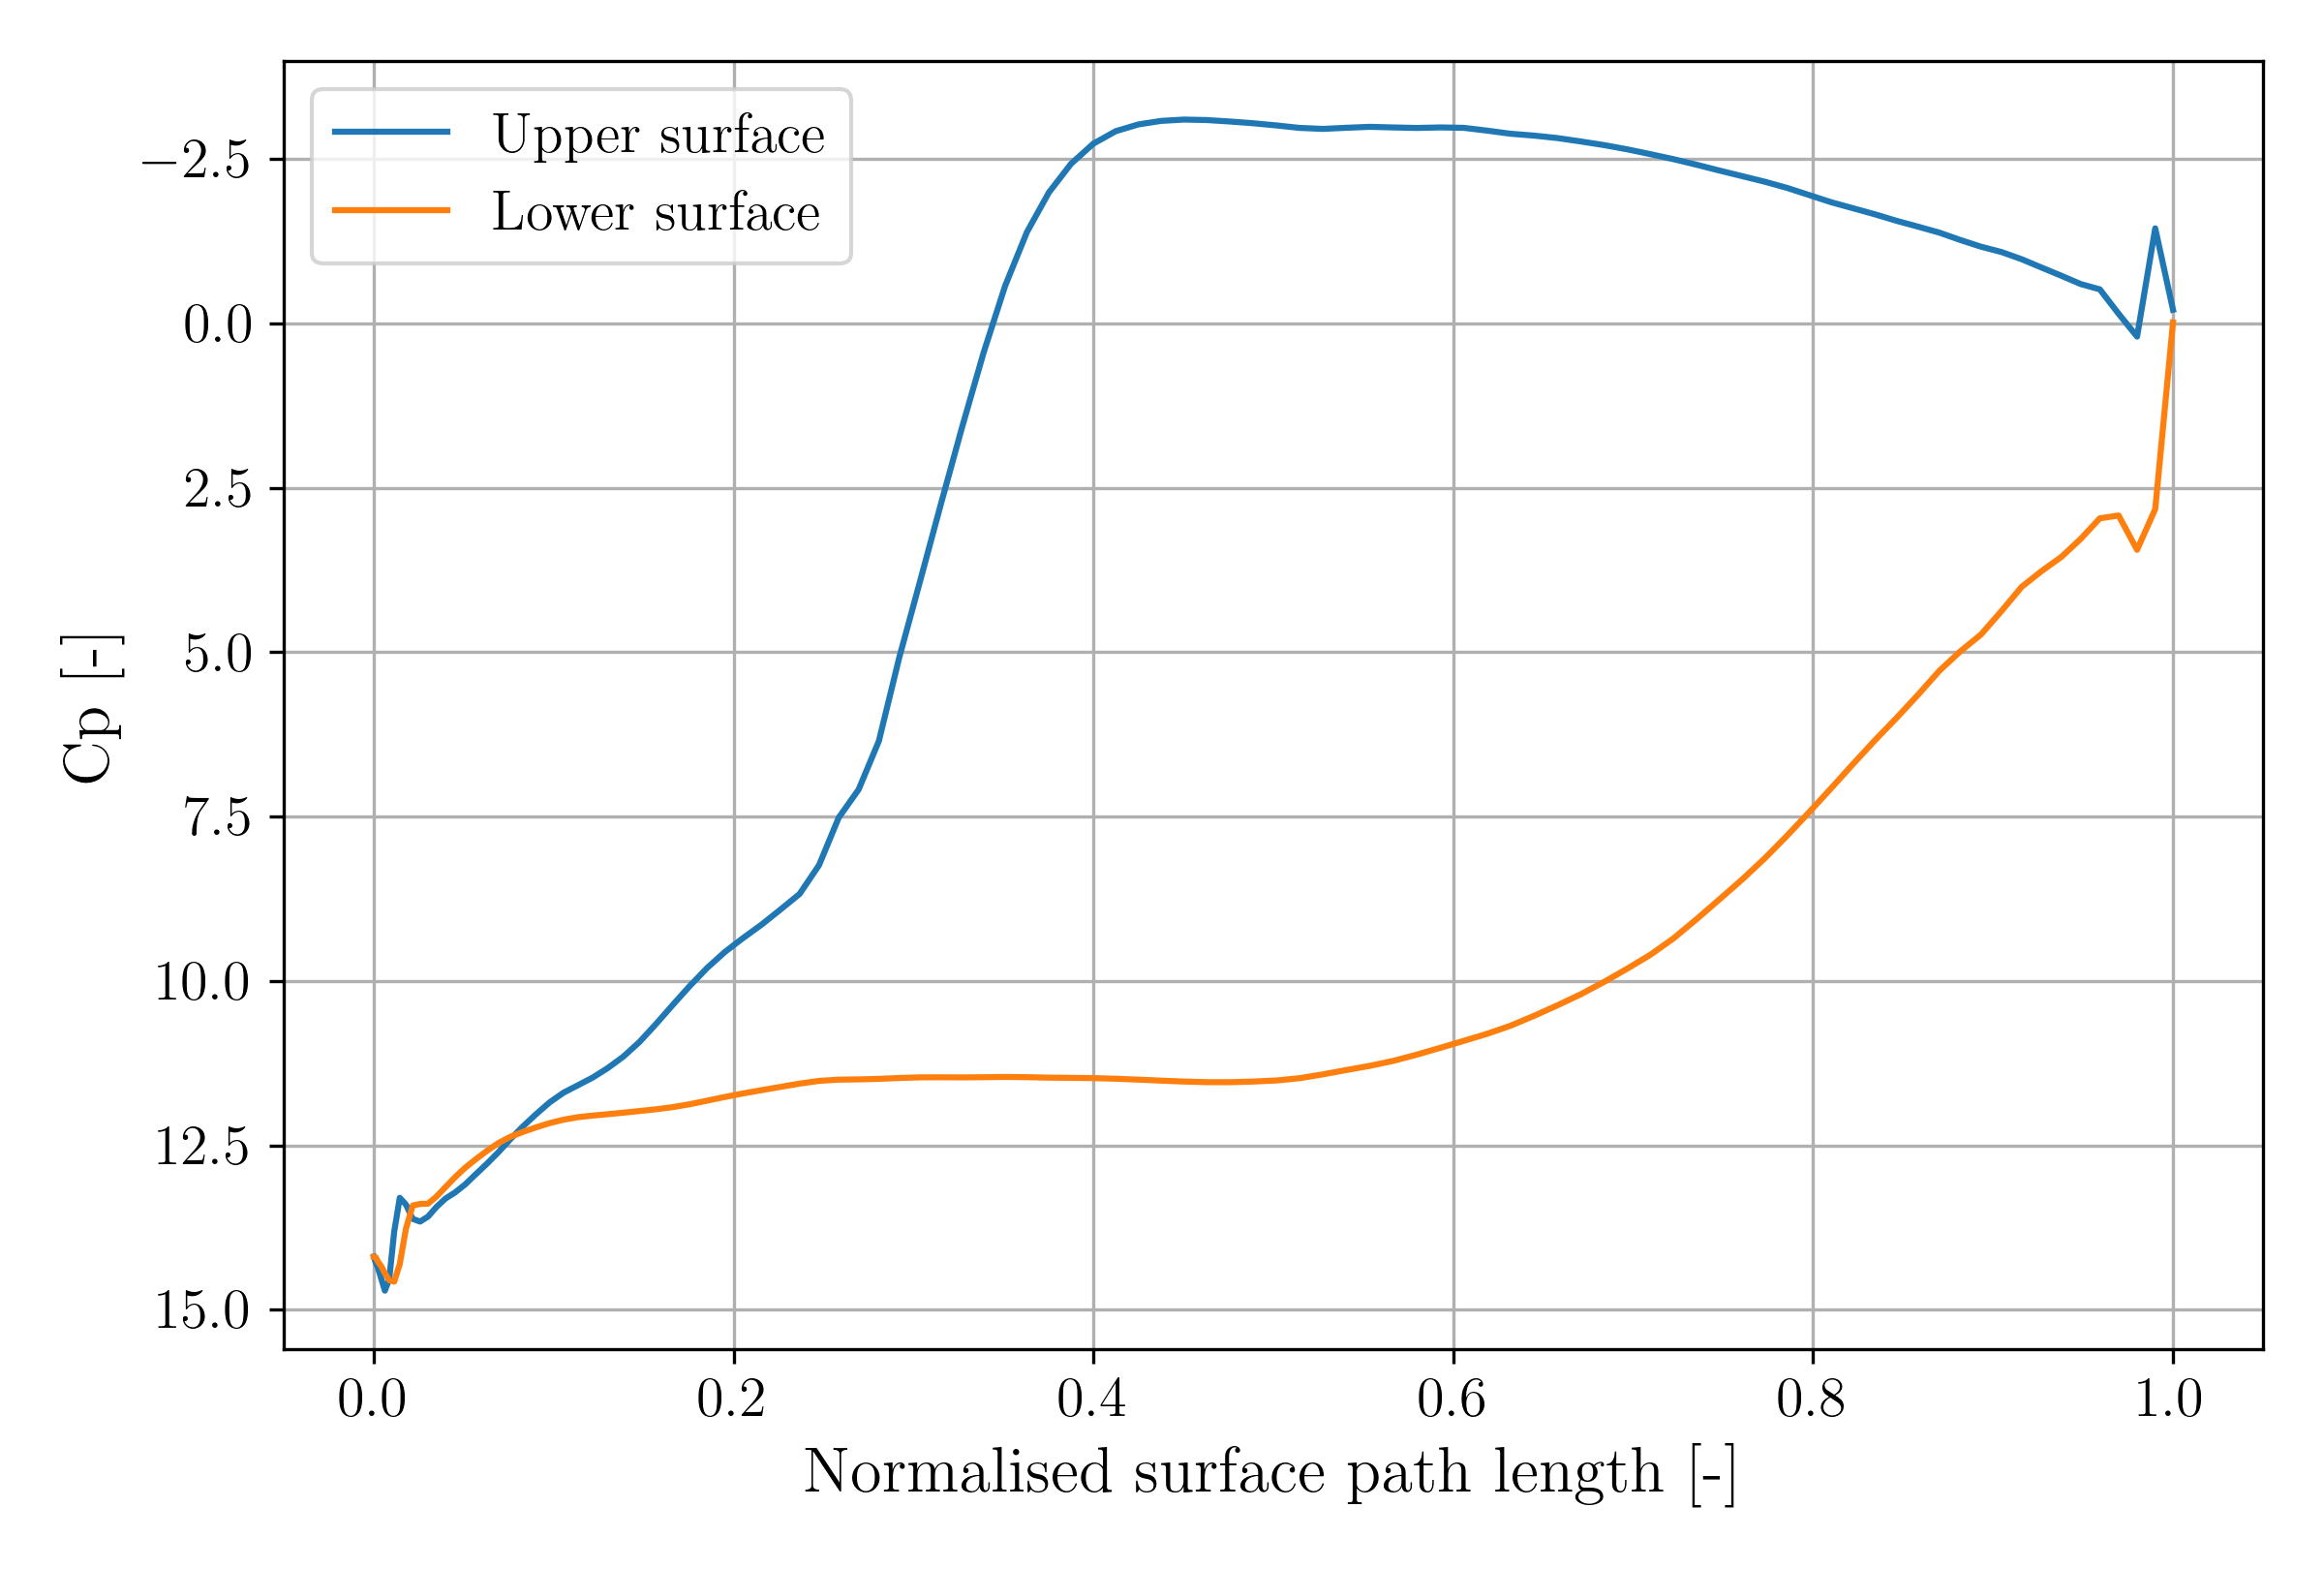
\includegraphics[width=0.99\textwidth]{figures/turbine_c_surface_cp.png}
        \caption{}
        \label{fig:turbine_c_surface_cp}
    \end{subfigure}
    \caption{Turbine\_c test case results}
\end{figure}

\begin{figure}[H]
    \centering
    \begin{subfigure}{0.44\textwidth}
        \centering
        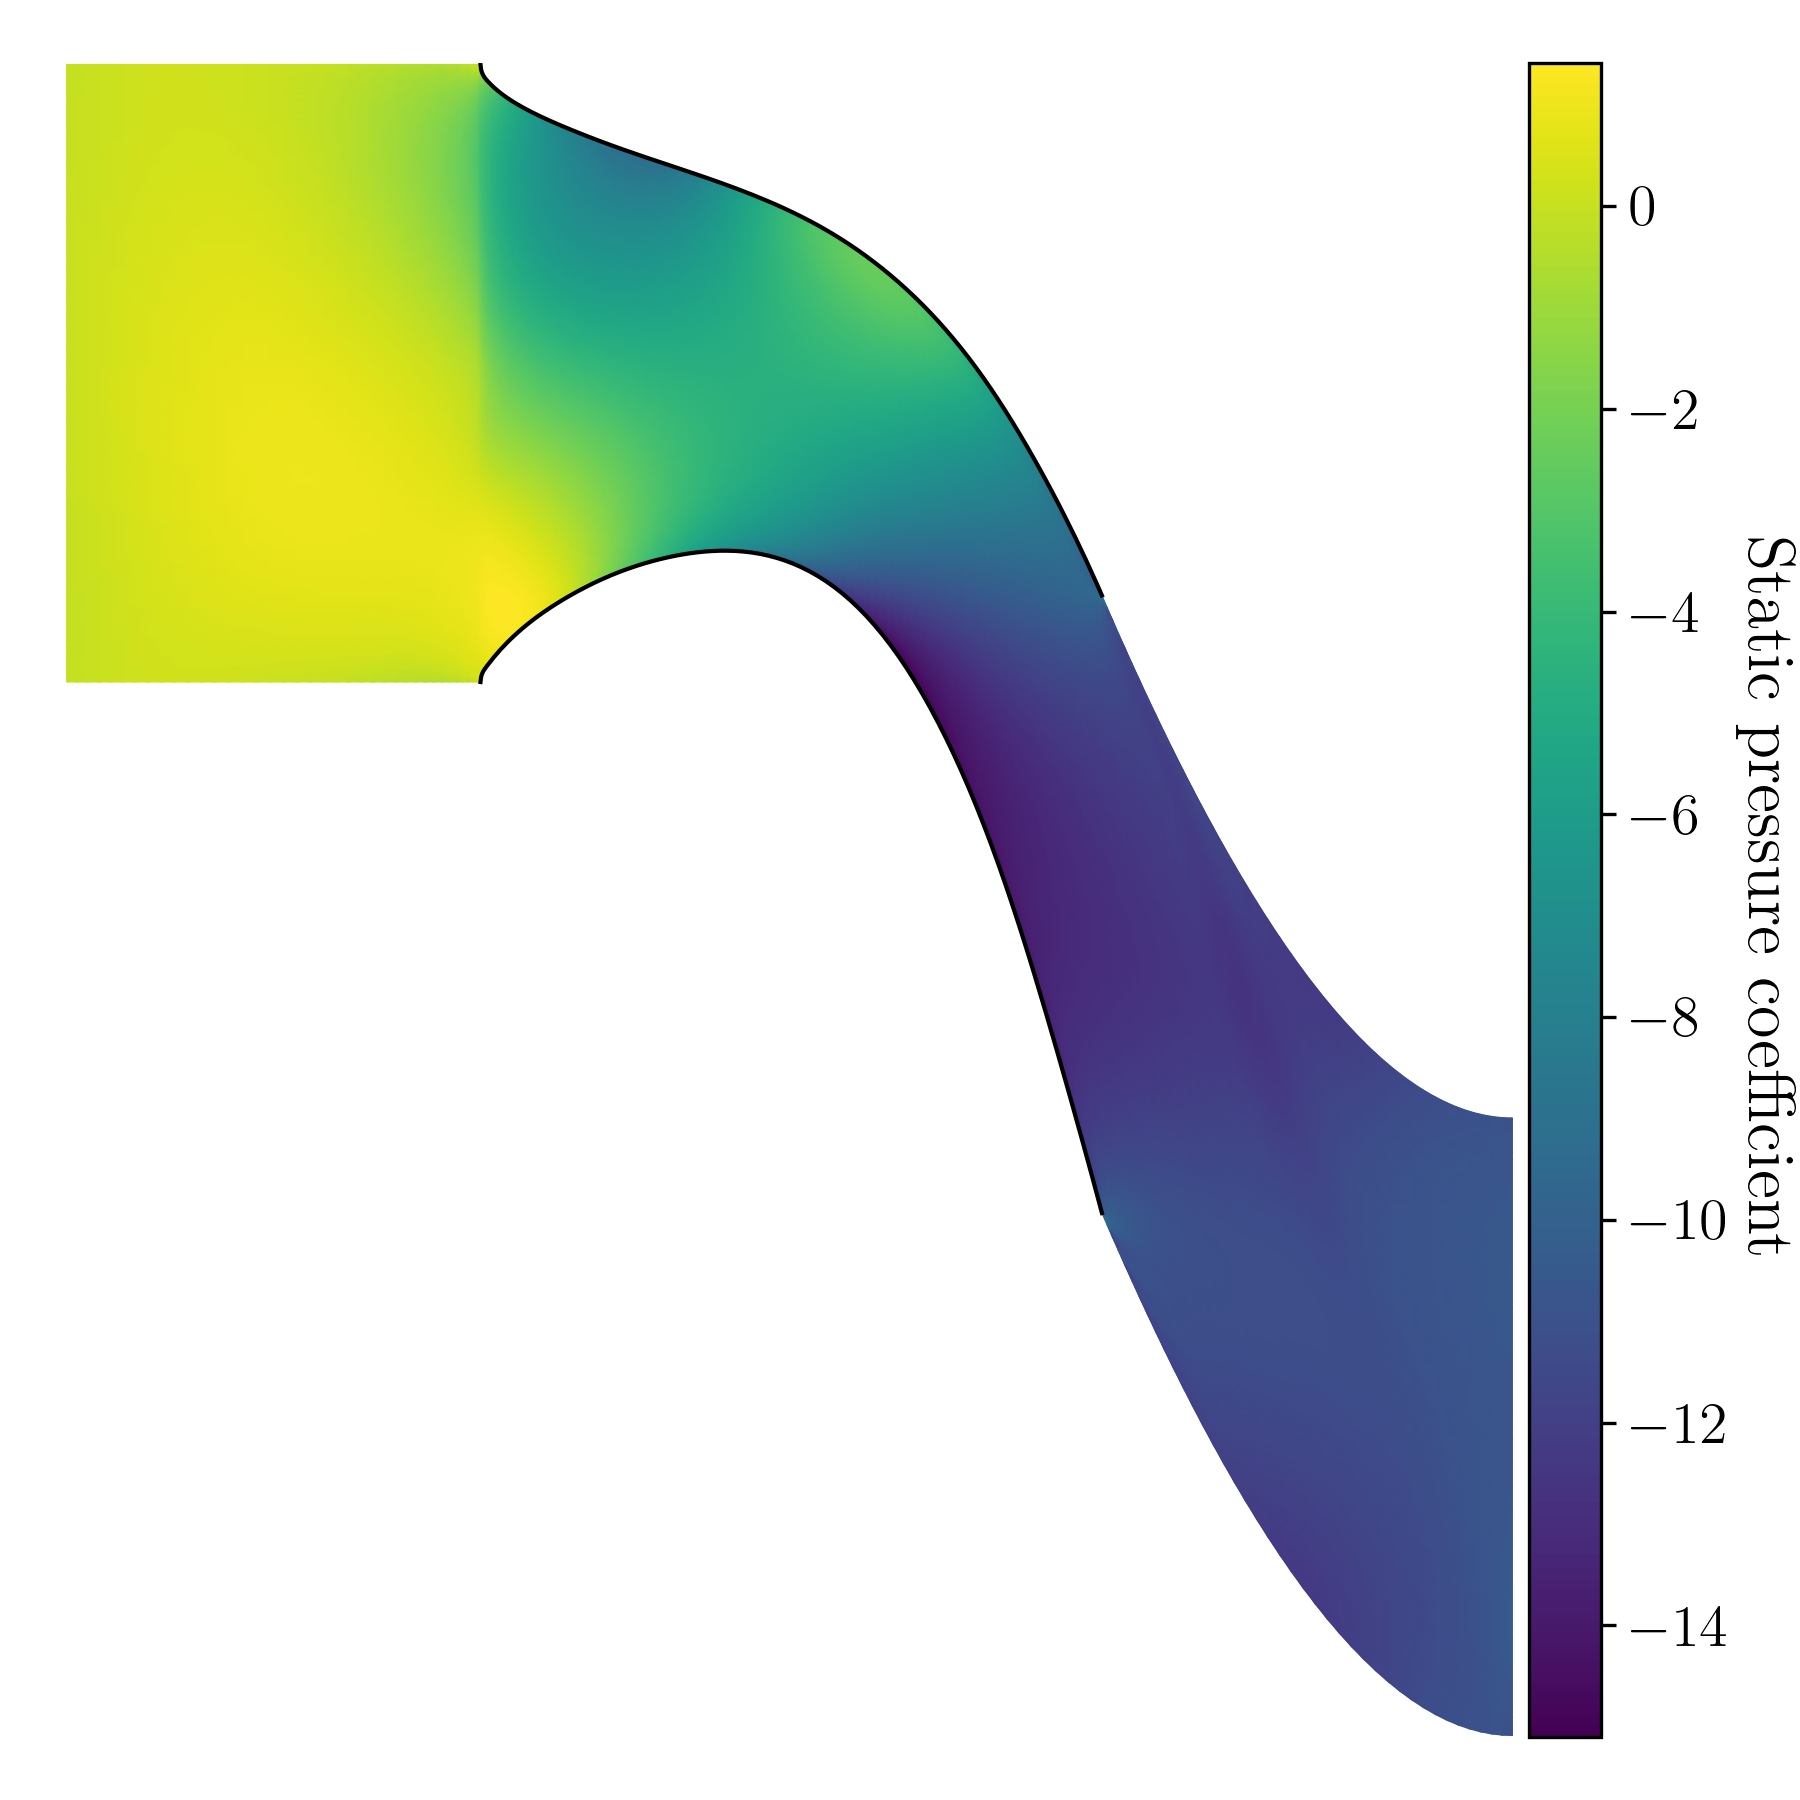
\includegraphics[width=0.99\textwidth]{figures/turbine_h_cp.png}
        \caption{}
        \label{fig:turbine_h_cp}
    \end{subfigure}
    \begin{subfigure}{0.55\textwidth}
        \centering
        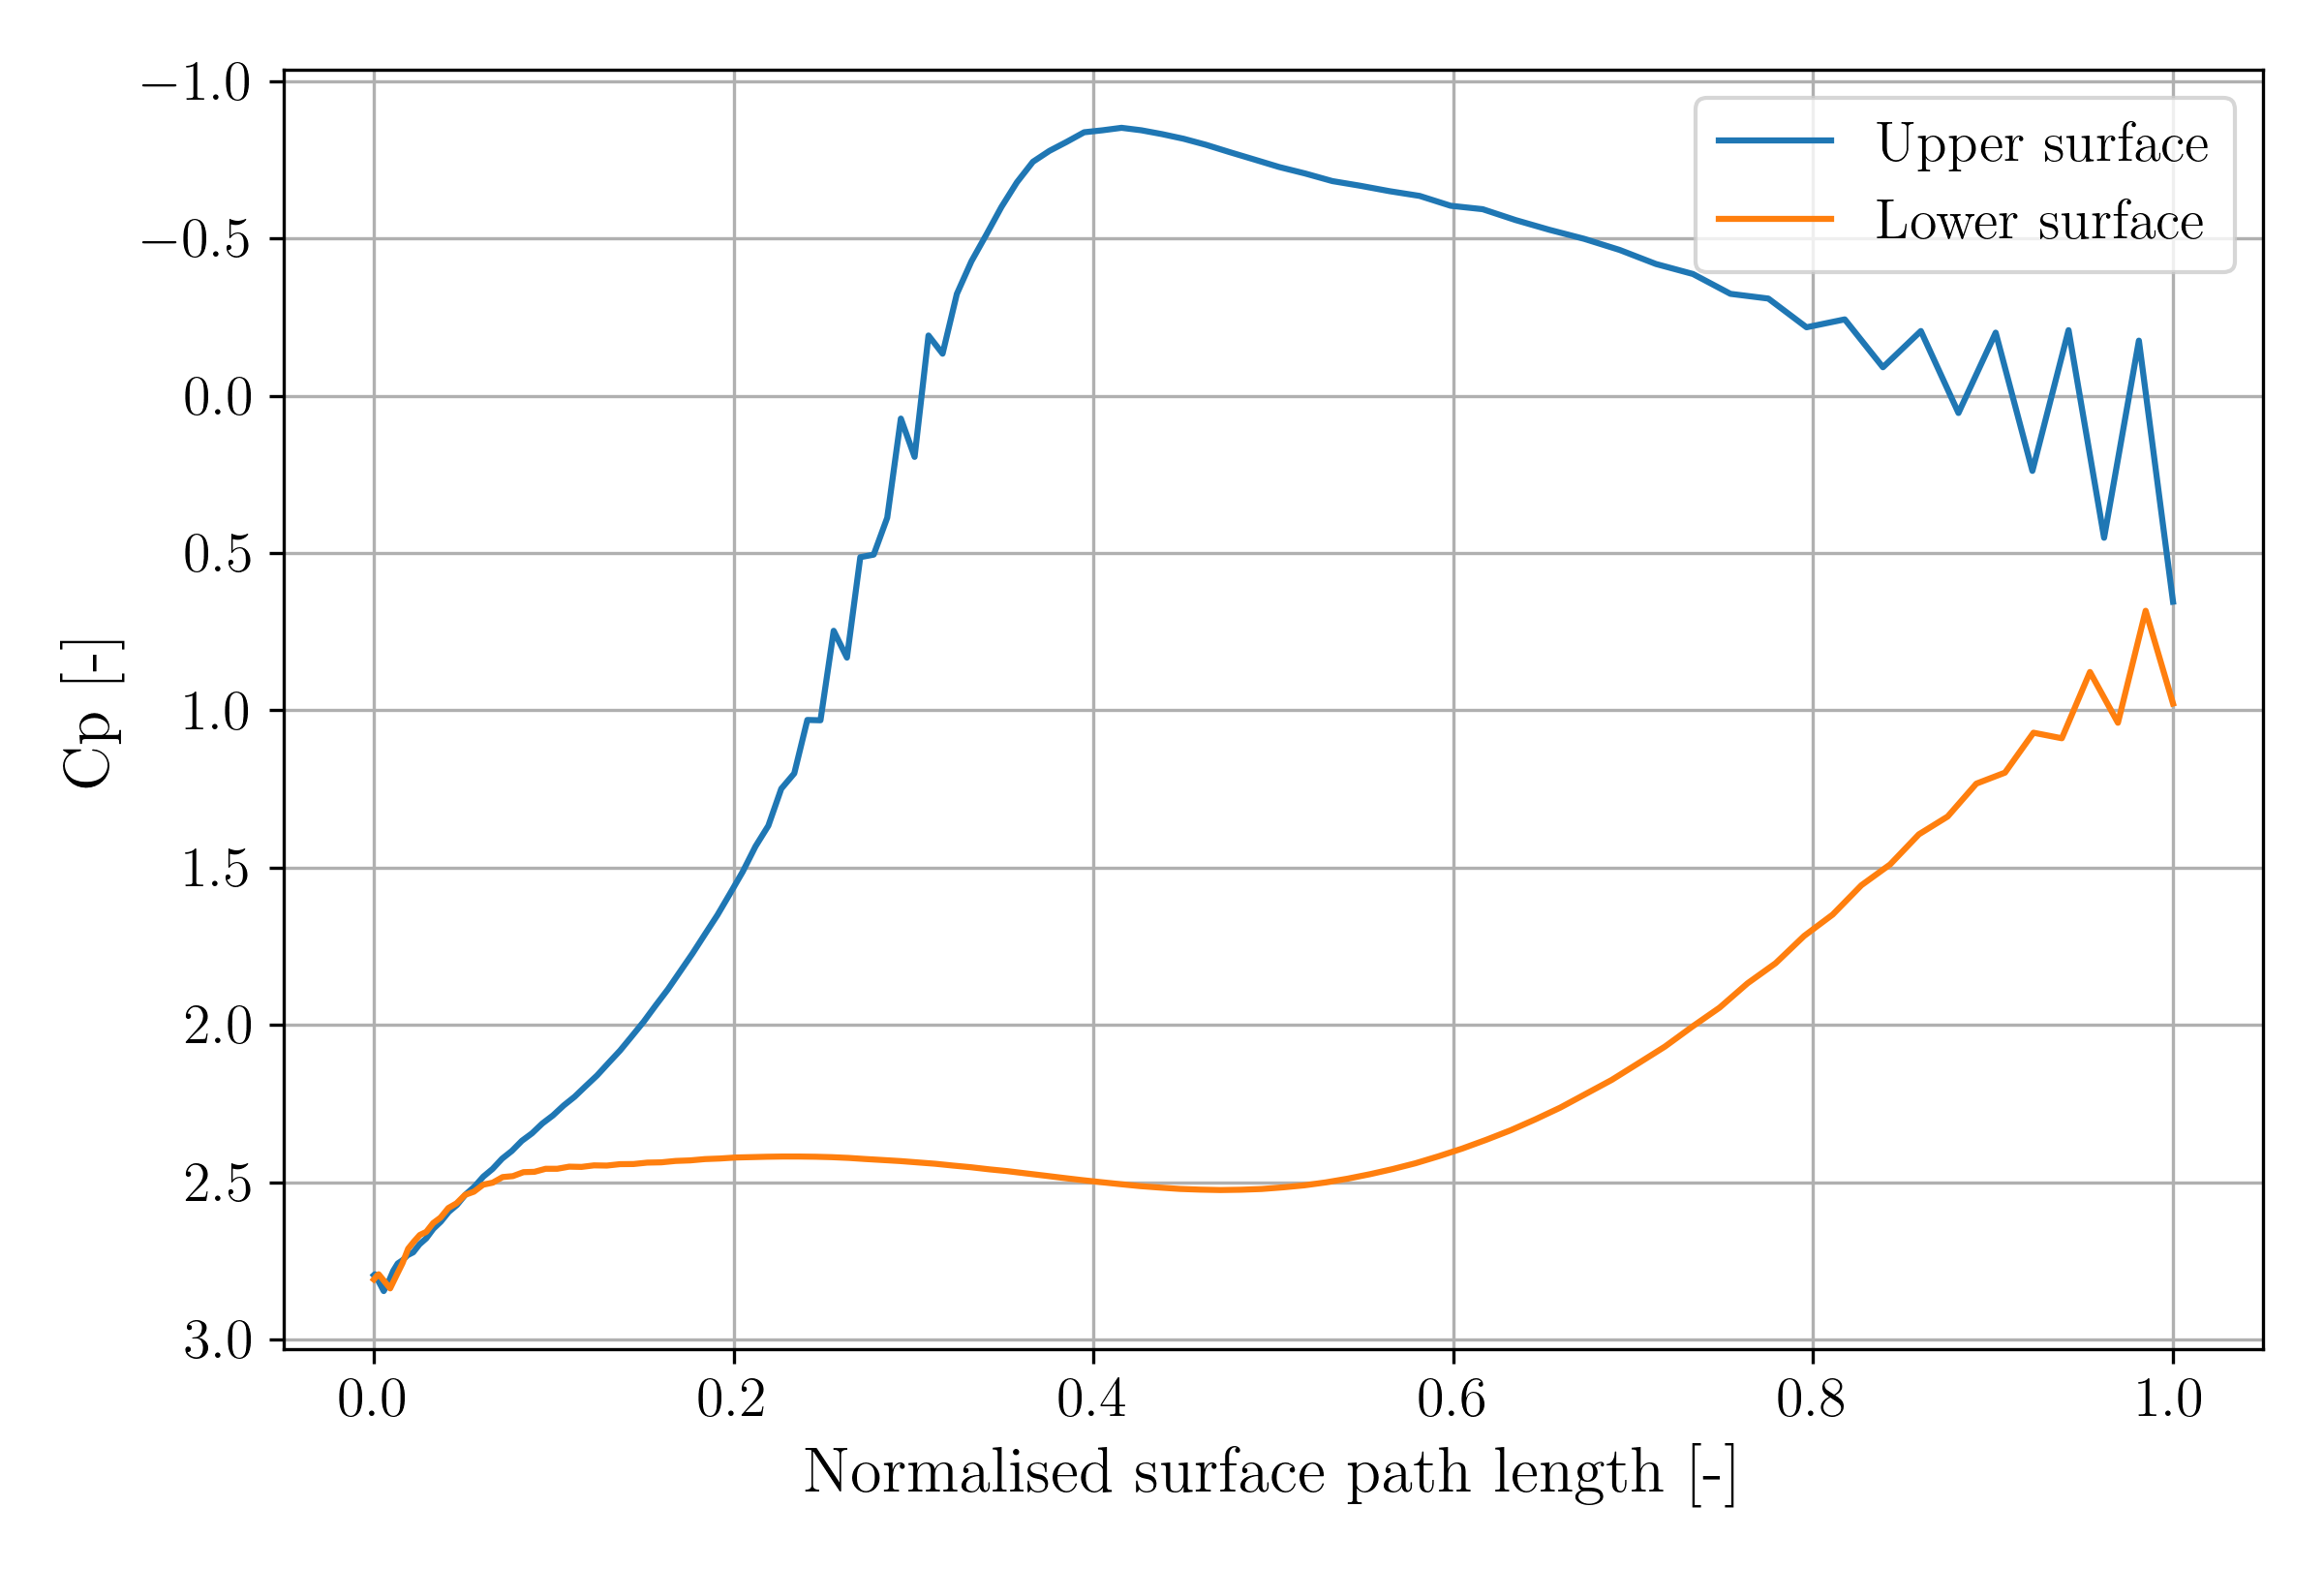
\includegraphics[width=0.99\textwidth]{figures/turbine_h_surface_cp.png}
        \caption{}
        \label{fig:turbine_h_surface_cp}
    \end{subfigure}
    \caption{Turbine\_h test case results}
\end{figure}

\section{Discussion}
% two pages that doesnt repeat interim

\subsection{Improvements}

Individual improvements were tested to see how they affected the solver.

Figures \ref{fig:improvements_cfl_residual} and \ref{fig:improvements_ni_residual} show the temporal and spatial accuracy of the solver for the various improvements.
The default solver is shown with no improvements and has the same first order temporal and second order spatial accuracy.
It is clear from the gradients that none of the improvements change the order of accuracy of the final steady state solution compared to the default solver.
It can be also seen that deferred correction improves the accuracy which is to be expected from the reduced artificial smoothing.
The same plateau in accuracy is observed for larger meshes due to floating point errors limiting the accuracy of area and spatial derivatives.
Again the deviation is also observed for the smallest mesh sizes which is thought to be due to boundary conditions applied over significant sections of the mesh.
The graphs also show only the converged runs for same logarithmic spacing of \texttt{cfl} and \texttt{ni}.
More missing points indicate instability of the parameters and it can be seen that at high \texttt{cfl} the spatially varying timestep and deferred correction both reduce the stability of the default solver.
The spatially varying timestep clearly reduces the stability as the most unstable cell is being updated by a larger local timestep than the previous smaller global timestep.
The deferred correction cancels out the artificial viscosity and so when run with the same \texttt{sfac} as the default case, the final smoothing is reduced which is shown to reduce stability at high \texttt{cfl} numbers \cite{interim}.

The relation of the runtime to \texttt{cfl} and \texttt{ni} is shown in figures \ref{fig:improvements_cfl_time} and \ref{fig:improvements_ni_time}.
Most of the improvements show the same temporal runtime order as the default ($\mathcal{O}(\texttt{cfl}^{-1/2})$) with the exception of the deferred correction.
The small region shows a runtime inversely proportional to \texttt{cfl}. %TODO
The Runge Kutta improvement shows a noticeable increase in runtime at the same \texttt{cfl} which is expected due to the increased number of intermediate timesteps.
This method also increases stability for larger \texttt{cfl} timesteps, allowing faster convergence and reducing the overall runtime.
From figure \ref{fig:improvements_ni_time} the spatial runtime order is the same first order as the default solver for all improvements.
At high \texttt{cfl} numbers and low \texttt{ni}, a plateau in runtime is observed which convergence before the minimum number of iterations to meet the convergence criteria discussed earlier.
This is most apparent for the small mesh sizes where convergence occurs in significantly fewer iterations.


The combination of all the improvements are then tested to see how they affect the solver.

Figure \ref{fig:cfl_sfac_dro_avg} shows the effect of \texttt{cfl} and \texttt{sfac} on the stability and residual error (accuracy) of the solver.
When compared to the same figure for the default solver in the interim report \cite{interim}, the improvement show stability at much higher \texttt{cfl} numbers.
It also shows stability at much lower \texttt{sfac} numbers which is thought to be due to the inclusion of residual averaging.


\subsection{NACA airfoils}

Figure \ref{fig:cl_alpha} shows the lift coefficient against angle of attack for the NACA0012 and NACA2412 airfoils.
The graph shows strong linear relationship for nearly all angles of attack.
From invicid theory, these lift coefficient should be linear with angle of attack with gradient $ 2\pi $.
However, the gradient the linear region is 

% discuss Kutta condition 
% not necessary to explicitly apply 
% because the artificial viscosity of the solver is enough to make the flow leave the trailing edge smoothly



\subsection{Turbine}

Theres two turbine cases, turbine\_c and turbine\_h which represent the same geometry but with different mesh layouts.


The results shown in figures \ref{fig:turbine_c_cp} and \ref{fig:turbine_h_cp} show the pressure coefficient for the turbine cases.
The run settings shown in table \ref{tab:default_params} are set to values measured from a real turbine experiment \cite{4A3_lab}.

\section{Summary}

\begin{thebibliography}{9}

    \bibitem{handout}
    J. V. Taylor
    \emph{4A2 Computational Fluid Dynamics: Writing an Euler Solver}
    University of Cambridge,
    2024.

    \bibitem{interim}
    L. W. Pender
    \emph{4A2 Interim Report}
    University of Cambridge,
    2024.

    \bibitem{solve_ODE_nonstiff}
    Hairer, Ernst et al.
    \emph{Solving ordinary differential equations I: Nonstiff problems, Berlin, New York}
    Springer-Verlag, Berlin, 1993

    \bibitem{4A3_lab}
    L. W. Pender
    \emph{4A3 Turbomachinary Laboratory Report}
    University of Cambridge,
    2024.
  
\end{thebibliography}

\section{Appendix}

\subsection{Software}

\begin{figure}[H]
    \centering
    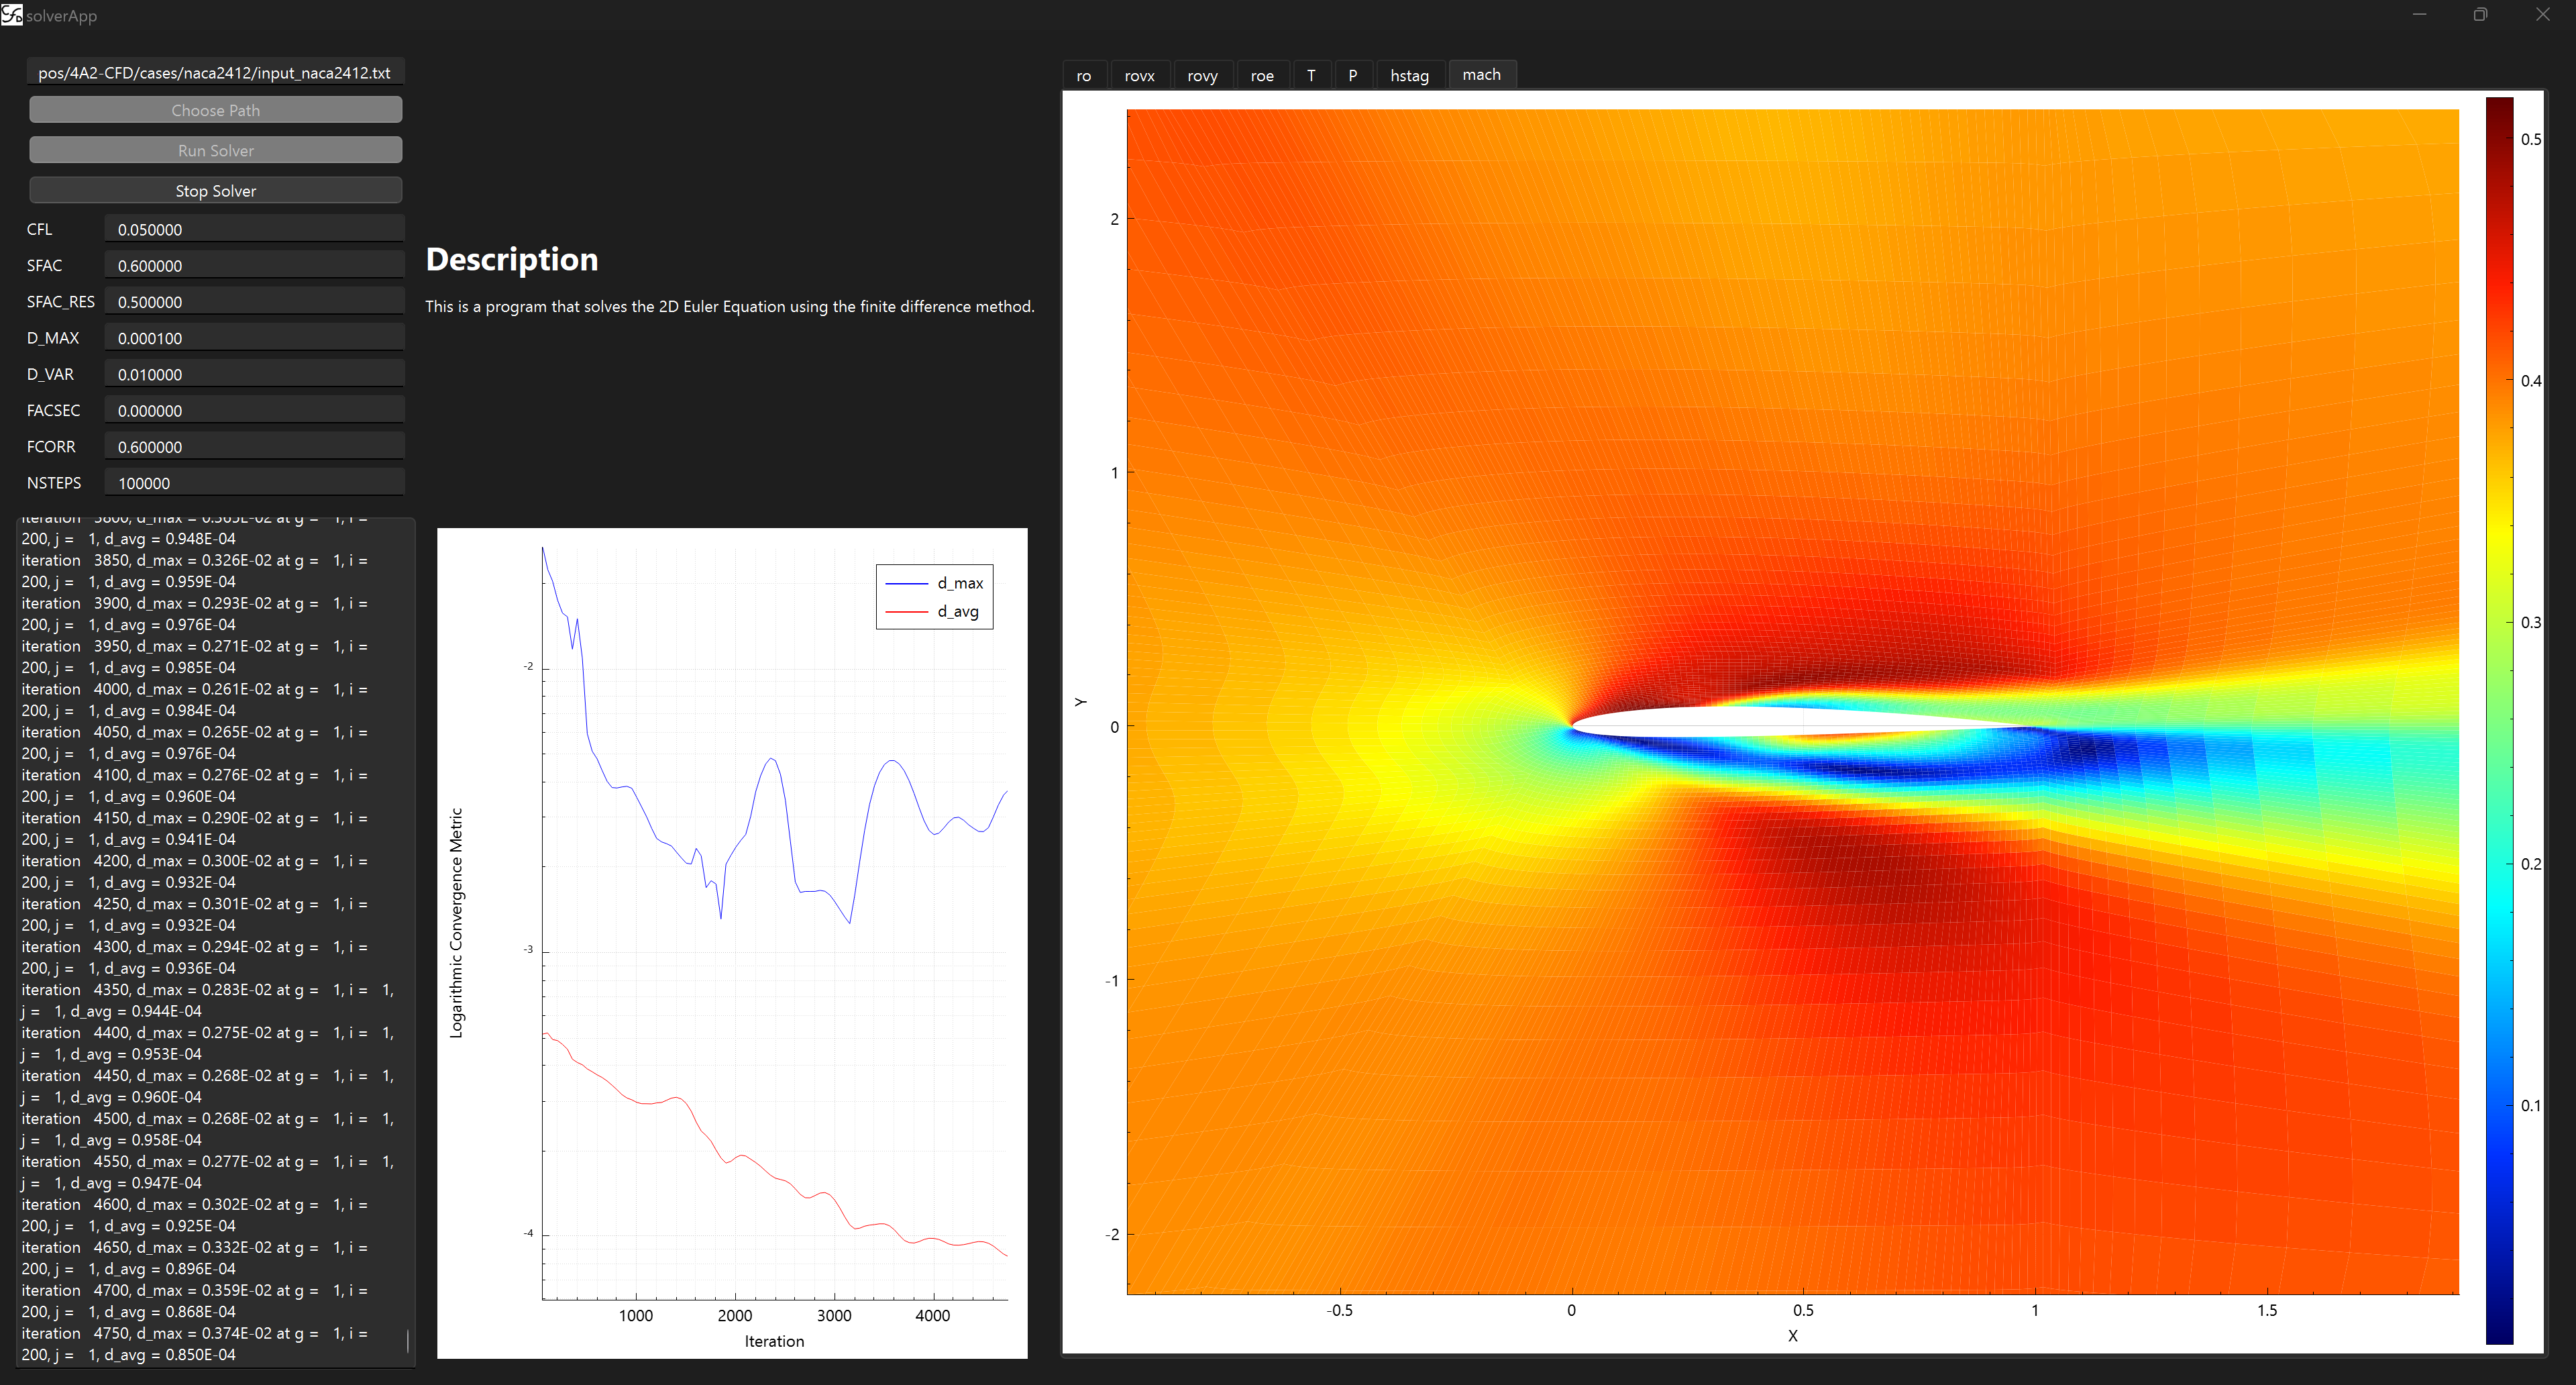
\includegraphics[width=0.7\textwidth]{figures/software.png}
    \caption{Software GUI}
    \label{fig:software}
\end{figure}

\subsection{Worker runtime enviroment}

A worker directory folder is created in the following format:
% directory tree for bump worker
\begin{figure}[H]
    \dirtree{%
    .1 1.
    .2 bump.
    .3 input\_bump.txt.
    .3 conv\_bump.csv.
    .3 out\_coord\_bump.bin.
    .3 out\_final\_bump.bin.
    .3 geom\_bump.txt.
    .3 out\_guess\_bump.bin.
    .2 log.txt.
    }
    \caption{Worker directory structure}
    \label{fig:worker_dir}
\end{figure}

During setup \texttt{generate\_case} is called and the settings and geometry files are written to the case folder.
During runtime the \texttt{log.txt} acts as \texttt{stdout} for the program.
When the solver finishes then the out files are saved and processed using the postprocessing python functions.

\begin{lstlisting}[language=Python]
def run(self):
    self.setup_environment()
    with open(self.log_file, "w") as log:
        try:
            parsed_file = str(self.in_file).replace("\\", "/")
            t1 = time.time()
            subprocess.run([self.cfd_executable, "--path", parsed_file],
                            check=True,
                            stdout=log)
            t2 = time.time()
        except subprocess.CalledProcessError as e:
            print(f"Worker {self.worker_id} failed with error: {e}")
            return

    self.dt = t2 - t1
    results = self.parse_results()

    # Write results to the shared file in a thread-safe way
    with self.shared_lock:
        with open(self.shared_file, "a", newline="") as csvfile:
            writer = csv.writer(csvfile)
            writer.writerow(results)

    print(f"Worker {self.worker_id} finished.")
\end{lstlisting}

\subsection{Real turbine comparison}

\iffalse
\begin{figure}[H]
    \centering
    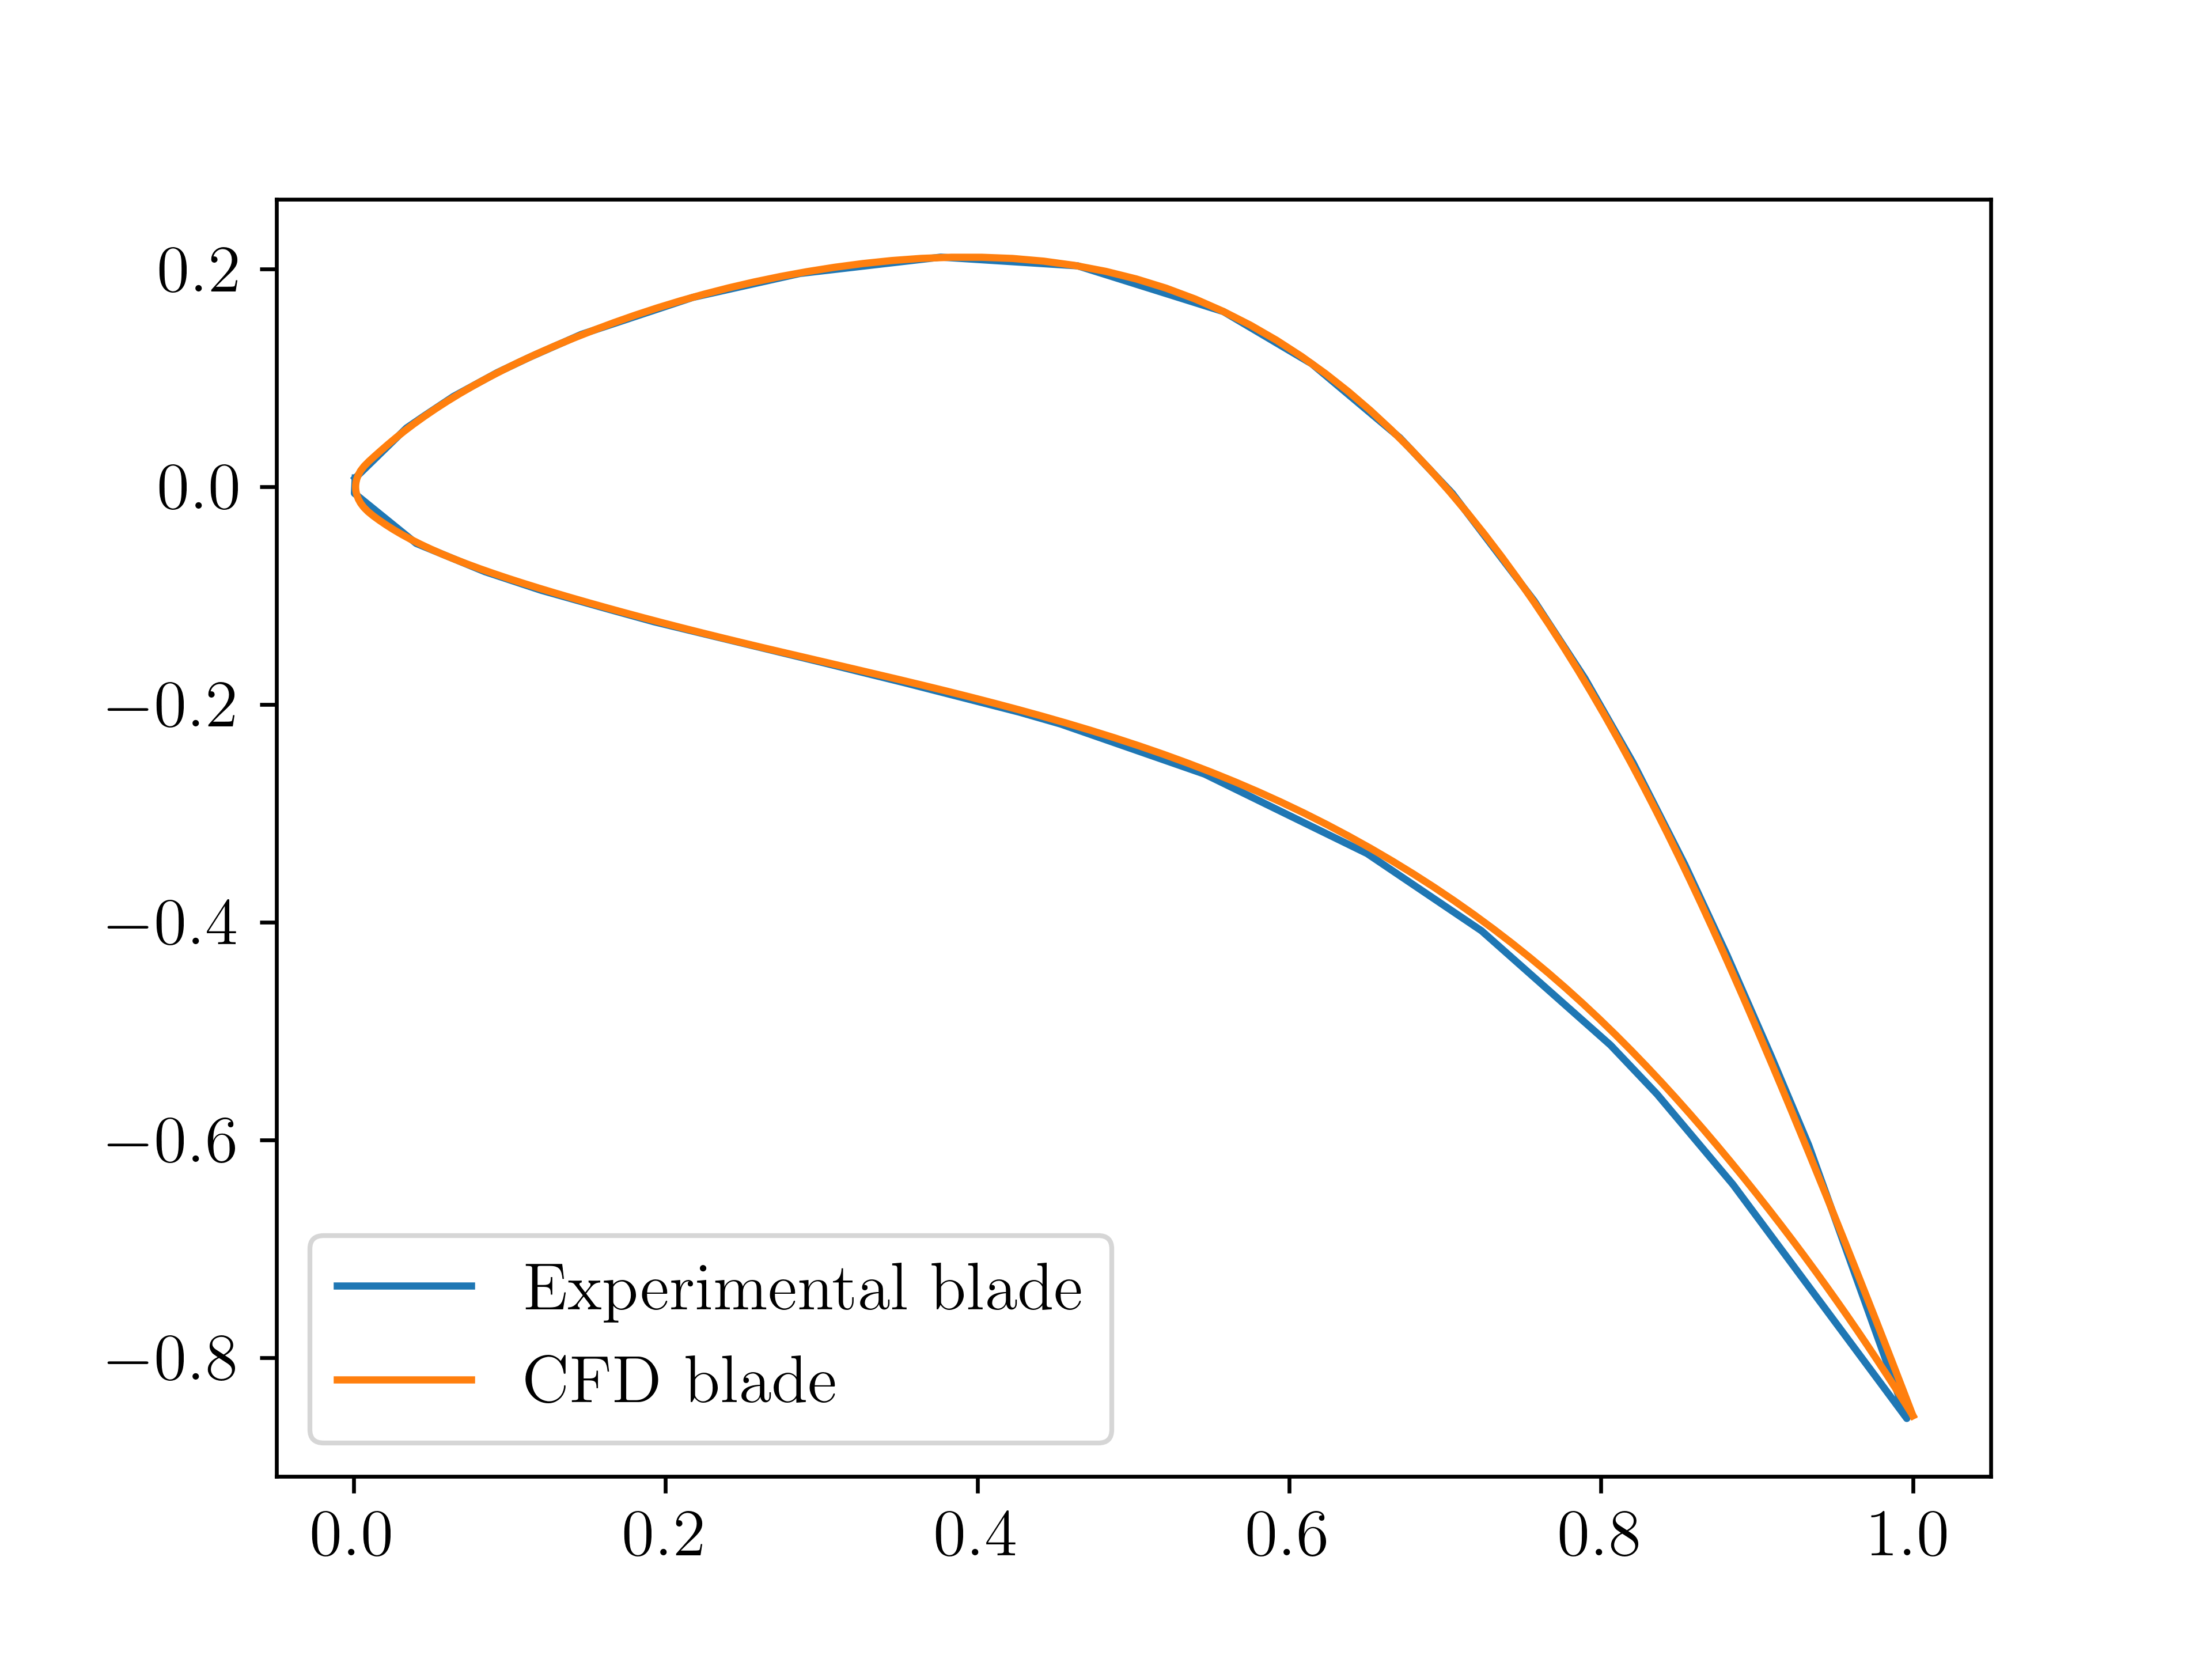
\includegraphics[width=0.6\textwidth]{figures/turbine_geometry.png}
    \caption{Comparison of turbine geometry}
    \label{fig:turbine_geometry}
\end{figure}
\fi

\begin{figure}[H]
    \centering
    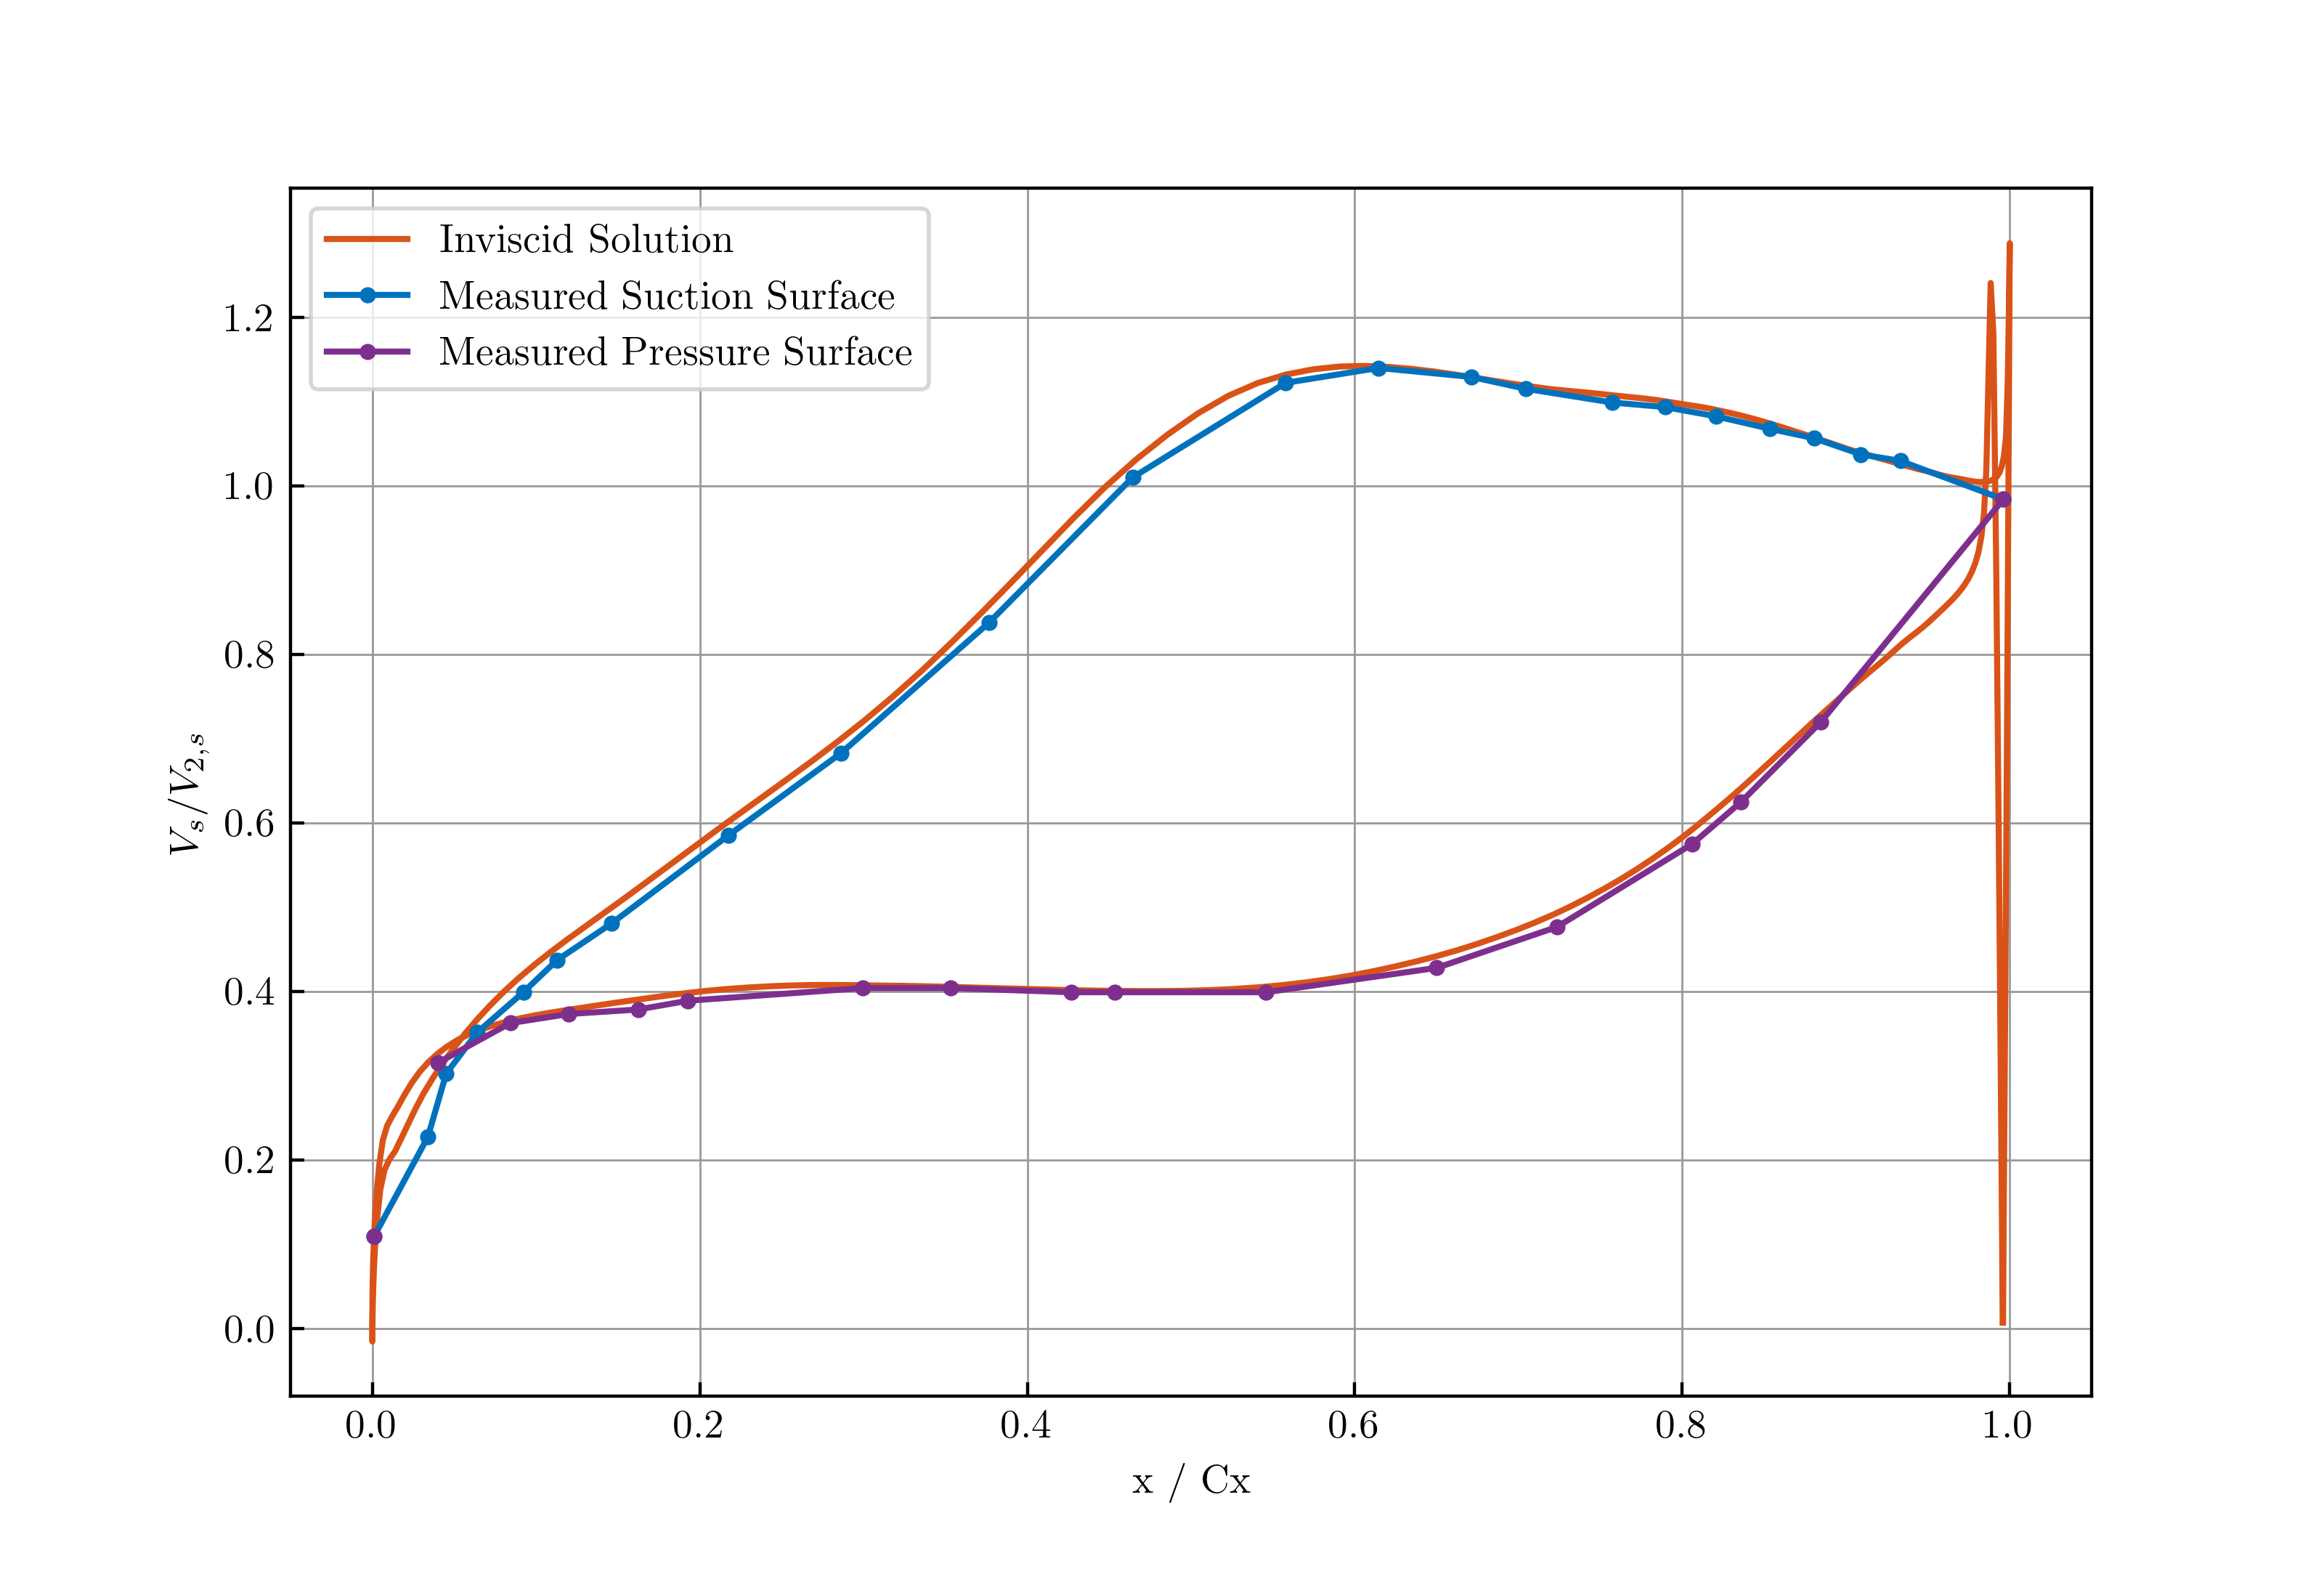
\includegraphics[width=0.99\textwidth]{figures/turbine_real.png}
    \caption{Real turbine data \cite{4A3_lab}}
    \label{fig:turbine_real}
\end{figure}

\end{document}